\documentclass{beamer}
% This is the file main.tex
%\usetheme{default}
\usetheme{Madrid}
%\usecolortheme{structure}
\usecolortheme[rgb={0.24,0.70,0.44}]{structure}
\usefonttheme[onlylarge]{structuresmallcapsserif}
\usefonttheme[onlysmall]{structurebold}
%\setbeamerfont{title}{shape=\itshape,family=\rmfamily}
%\setbeamercolor{title}{fg=red!80!white}
%\setbeamercolor{title}{fg=red!80!white,bg=red!20!white}

% Utilizamos el paquete para usar español
\usepackage[spanish]{babel}
% Utilizamos un paquete para gestionar los acentos
% y las e ¿es
\usepackage[utf8]{inputenc}
% amsmath y amssymb de la American Mathematical 
% Society (fórmulas matemáticas)
\usepackage{amsmath}
\usefonttheme[onlymath]{serif}
%Para que reconozca el entorno verbatim
\usepackage{fancyvrb}
%Definimos nuestra ruta para las imagenes
%Absoluto
%\graphicspath{ {/home/user/images/} }
%Relativo (recomendado) -> según
%https://es.sharelatex.com/learn/Inserting_Images#La_ruta_a_la_carpeta_de_im.C3.A1genes
\graphicspath{ {../media/} }


\title[Proyecto LAGO]{Electrónica rápida para el acondicionamiento de señales}
\subtitle{Universidad de La Serena \\ La Serena -- Chile}
\author[\texttt{@horacio\_arnaldi}]{Horacio Arnaldi \\ \texttt{{\href{mailto:arnaldi@cab.cnea.gov.ar}{arnaldi@cab.cnea.gov.ar}}}}
\institute[LabDPR - CAB - IB]{Laboratorio Detección de Partículas y Radiación \\ Centro Atómico Bariloche - Instituto Balseiro}
\date{}

\begin{document}

\begin{frame}
  \hspace*{0.5cm}
  
\includegraphics[height=0.18\textheight]{logos/cnea_logo} \hspace*{1cm}
  
\includegraphics[height=0.18\textheight]{logos/balseiro_logo} \hspace*{1cm}
  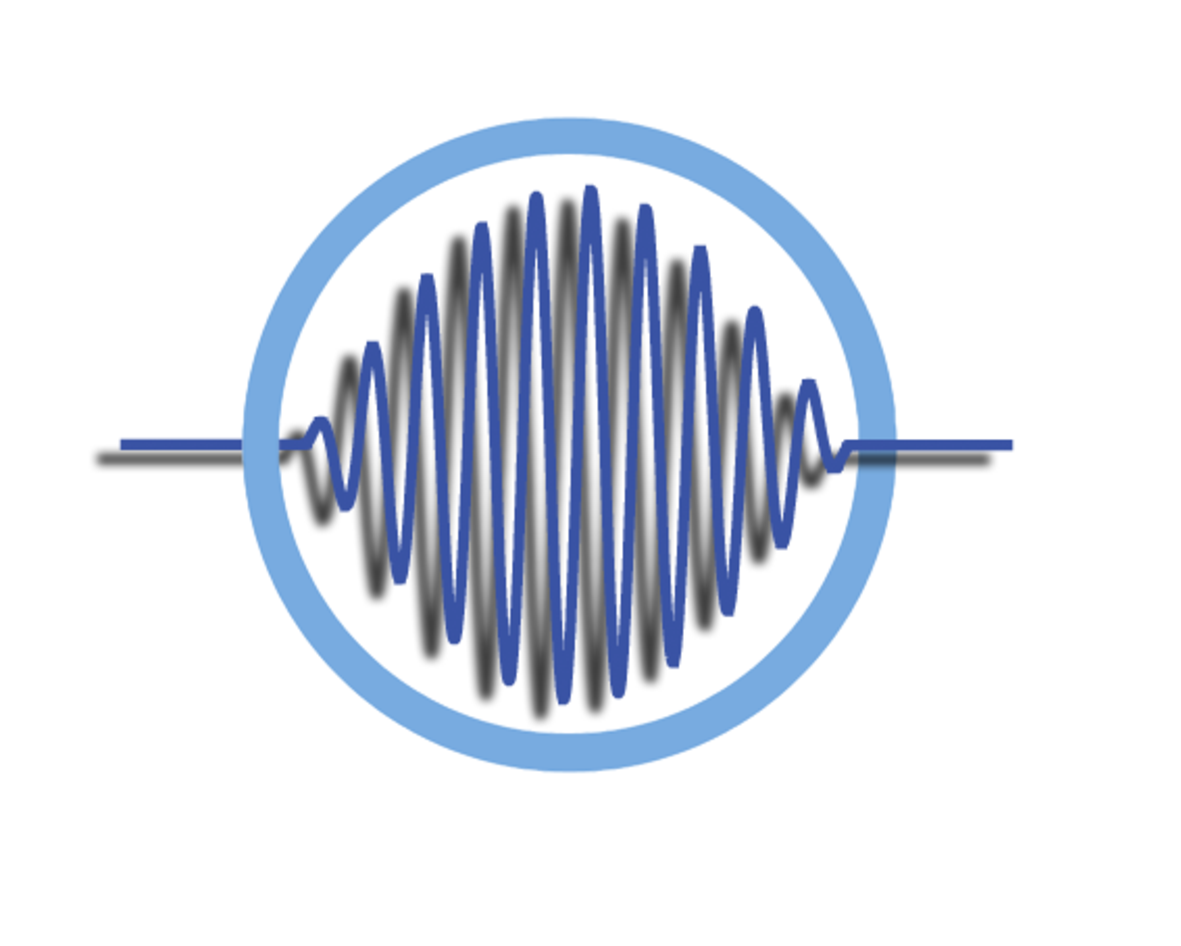
\includegraphics[height=0.18\textheight]{logos/LabDPR_logo} \hspace*{1cm}
  
\includegraphics[height=0.18\textheight,width=0.15\textwidth]{logos/lagologo}

  \titlepage

\end{frame}

\begin{frame}
  \frametitle{Contenido}
 \setcounter{tocdepth}{1} %para incluir solo las secciones en el TOC
  \tableofcontents
%  \tableofcontents[pausesections]
\end{frame}

%------------------------------------------------------------------------------
\section{Introducción}
%------------------------------------------------------------------------------
\begin{frame}
\begin{center}
\Huge{\color{blue}{Introducción}} \\
%\vspace*{5mm}
%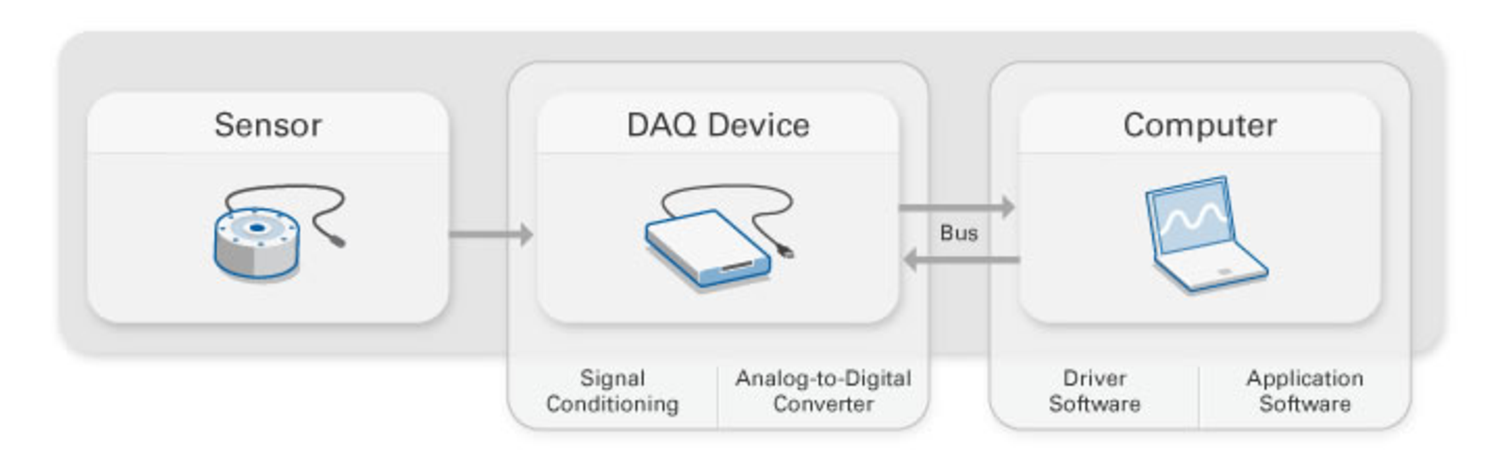
\includegraphics[width=\textwidth]{d2/daq_system_general}
\end{center}
\end{frame}

\begin{frame}
\frametitle{Introducción}
\only<1>{\fbox{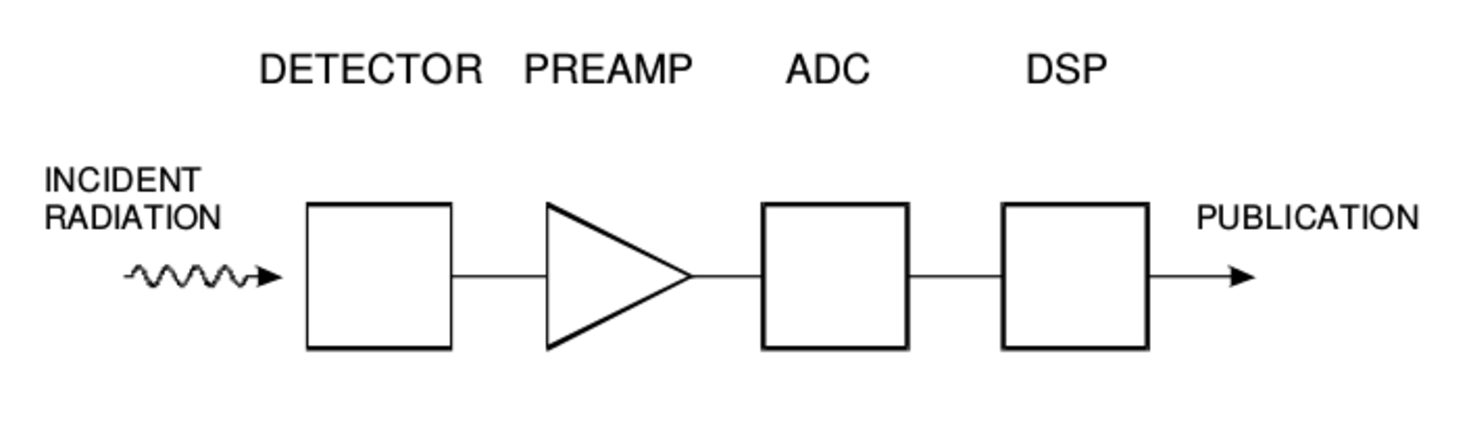
\includegraphics[width=\textwidth]{d1/block_diag_det_syst}}}
\only<2>{\fbox{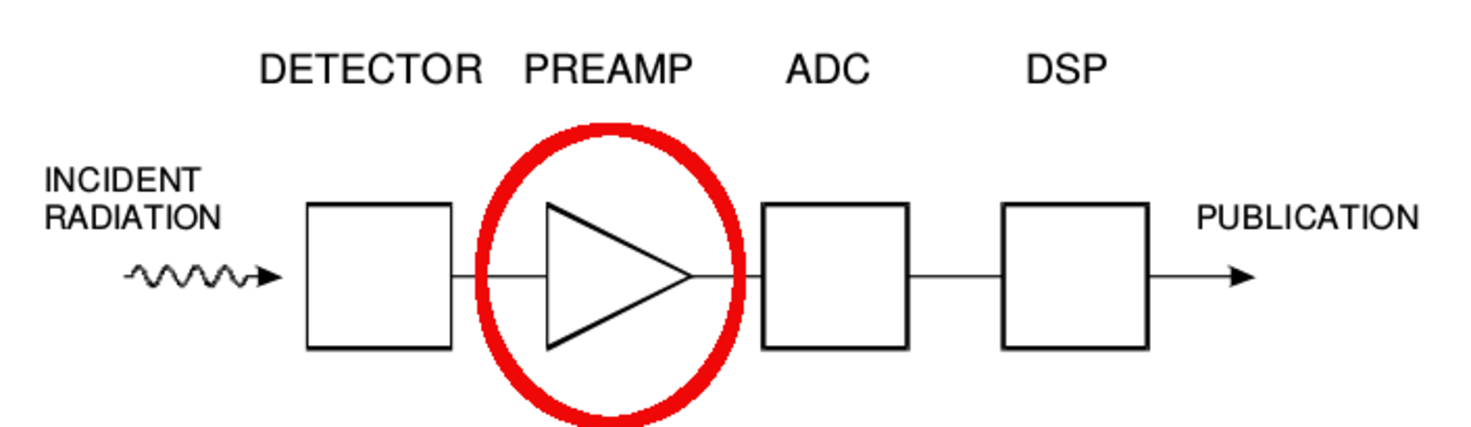
\includegraphics[width=\textwidth]{d1/block_diag_det_syst2}}}
\end{frame}

\begin{frame}
\frametitle{Propósito de los sistemas de procesamiento de pulsos}
\begin{alertblock}{}
\begin{enumerate}
\item Adquirir las señales eléctricas del detector ({\color[rgb]{0,0,1}típicamente pulsos
cortos de corriente})
\item Adaptar la respuesta temporal (es decir ``{\color{violet}conformar}'' el pulso de salida) del sistema para optimizar:
\begin{itemize}
\item Mínima señal detectable
\item Medición de la energía (magnitud de la señal)
\item Tasa de eventos
\item Tiempo de arribo (medición de tiempo)
\item Insensibilidad a la forma del pulso del detector
\item Alguna combinación de las anteriores
\end{itemize}
\alert{Generalmente no es posible optimizar varias a la vez $\rightarrow$
{\color{blue} compromisos}}
\item Digitalizar la señal y guardarla para un análisis posterior
\end{enumerate}
\end{alertblock}
\end{frame} 

\begin{frame}
\frametitle{Requerimientos adicionales, dependiendo de la aplicación}
\begin{block}{}
\begin{itemize}
\item Resistencia a la radiación
\item Bajo consumo
\begin{itemize}
\item Sistemas portables
\item Arreglos grandes de detectores, p. ej. Auger
\end{itemize}
\item Robustez
\item Costo
\end{itemize}
\end{block}
\end{frame} 

\begin{frame}
%Leo 11.1
\frametitle{Terminología de señales pulsadas}
\begin{itemize}
\item Electrónica moderna $\rightarrow$ variada información de la radiación
detectada
\item Se requiere procesamiento para extraer la información
\item P. ej. extraer información sobre la energía, determinar tiempos relativos
entre señales, etc.
\item Tomar decisiones sobre la \alert{aceptabilidad} del evento
\item Estandarización $\rightarrow$ CAMAC, NIM
\end{itemize}
\end{frame} 

\begin{frame}
\frametitle{Terminología de señales pulsadas}
\begin{itemize}
\item La codificación de la información se hace generalmente en forma de señales
de pulsos 
\item Son breves aumentos de corriente o voltaje en los que la información puede
estar contenida en una o más de sus características, por ejemplo, su polaridad,
amplitud, forma, su ocurrencia en el tiempo con relación a la presencia de otro
pulso o simplemente su mera presencia
\end{itemize}
\end{frame} 

\begin{frame}
\frametitle{Terminología de señales pulsadas}
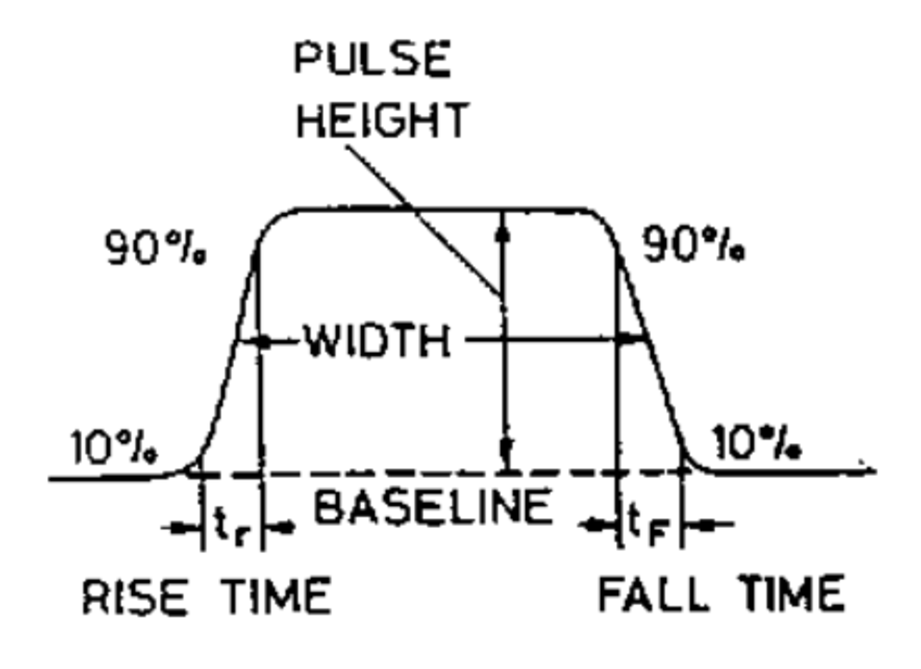
\includegraphics[width=0.5\textwidth]{d2/parametros_pulso}
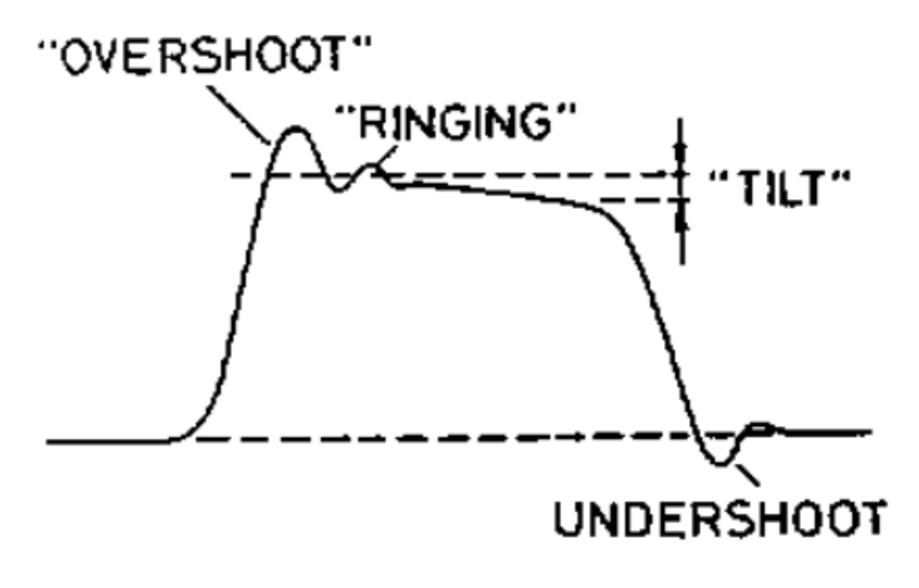
\includegraphics[width=0.5\textwidth]{d2/parametros_pulso2}
\end{frame} 

\begin{frame}
\frametitle{Terminología de señales pulsadas}
\begin{columns}
\begin{column}{0.5\textwidth}
\begin{enumerate}
\item Baseline (línea de base)
\item Altura del pulso o amplitud
\item Ancho del pulso
\item Leading edge
\item Falling edge
\item Rise time
\item Fall time
\item Unipolar o bipolar
\end{enumerate}
\end{column}
\begin{column}{0.5\textwidth}
\begin{center}
\only<1>{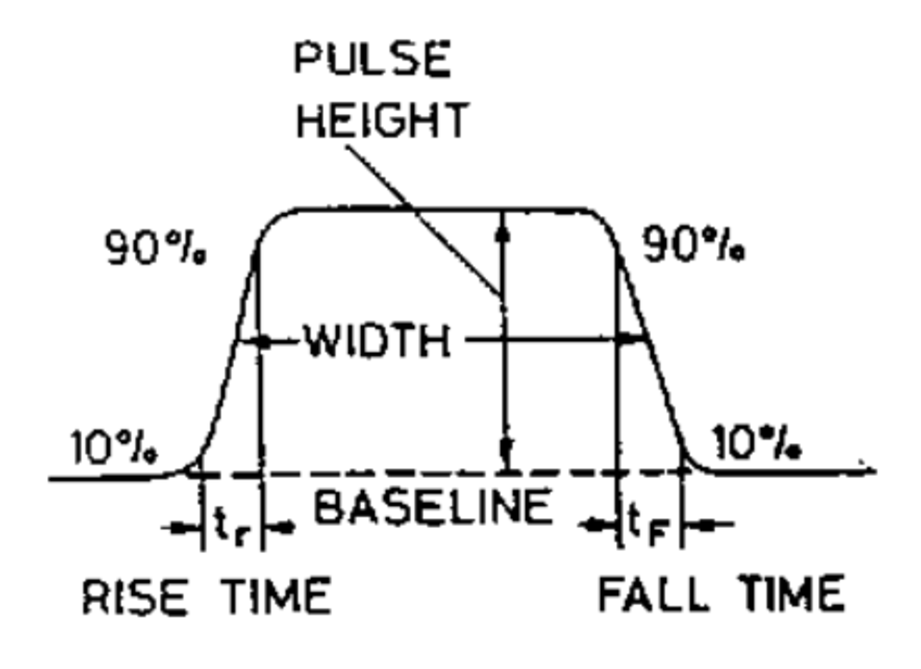
\includegraphics[width=0.8\textwidth]{d2/parametros_pulso} \\

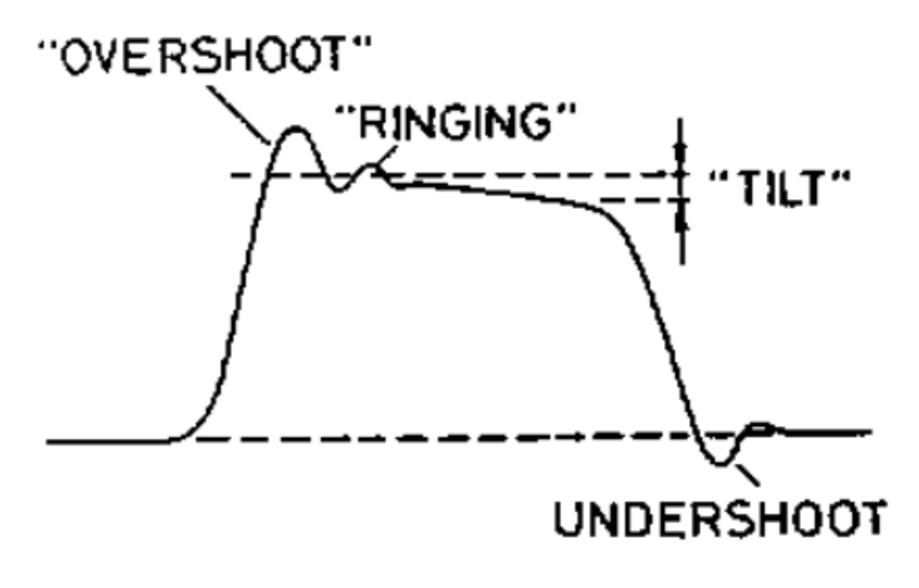
\includegraphics[width=0.8\textwidth]{d2/parametros_pulso2}}
\only<2>{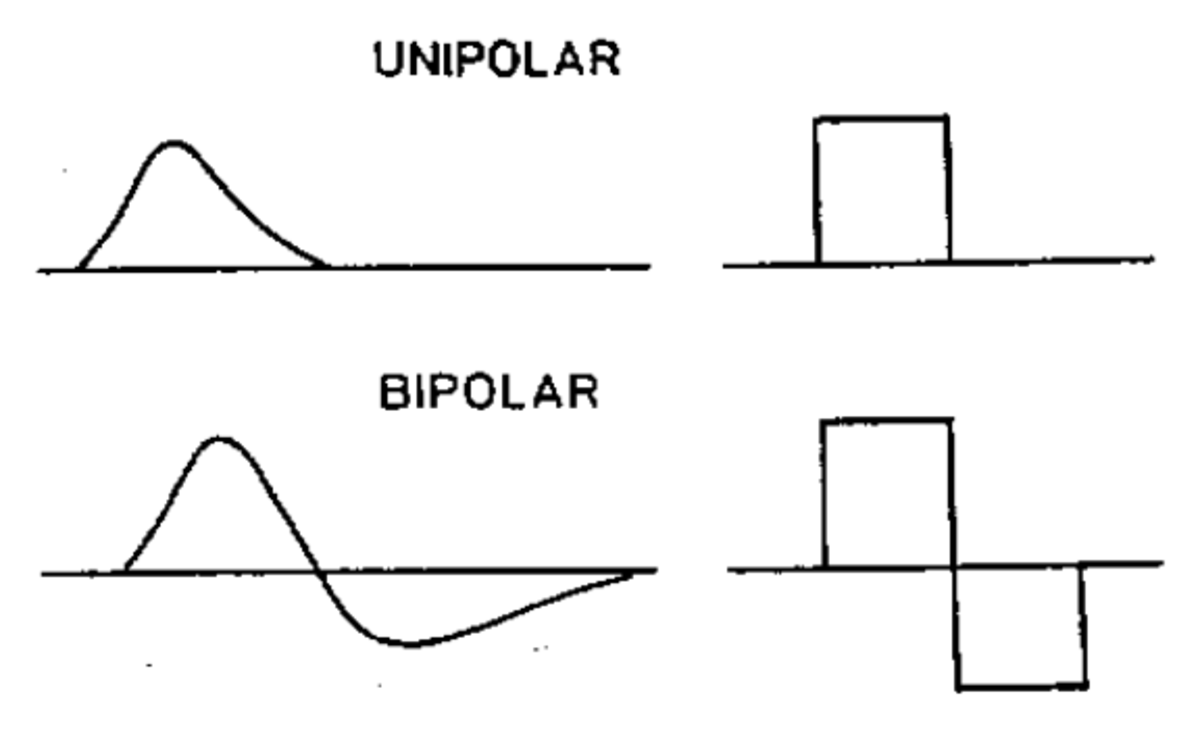
\includegraphics[width=\textwidth]{d2/unipolar_and_bipolar_pulse}}
\end{center}
\end{column}
\end{columns}
\end{frame} 

%\begin{frame}
%%FIXME: en la intro hablar sobre Nyquist fn = 2* fm, explicar lo que es oversampling
%\frametitle{Clasificación}
%\begin{block}{}
%\begin{itemize}
%\item Aparece el concepto de ``variable''
%\item Clasificación por {\bf características} y por {\bf tipo}
%\item Por característica: térmicos, radiación, fuerza, proporción, cantidad, geométricos
%propiedades físicas, composición química y eléctricos.
%\end{itemize}
%\end{block}
%\end{frame} 
%
%\begin{frame}
%\frametitle{Definiciones (Cont.)}
%\begin{columns}
%\begin{column}{0.50\textwidth}
%\begin{block}{Electrónica dedicada para Auger}
%\begin{itemize}
%\item Poco flexible 
%\item Información limitada
%\item Número limitado de UBs (\alert{Unified Boards})
%\item Comunicación de datos por puerto serie
%\item Tiempos de adquisición largos
%\item Poco volumen de almacenamiento
%\item Sin control línea de base	
%\end{itemize}
%\end{block}
%\end{column} 
%\begin{column}{0.50\textwidth}
%\fbox{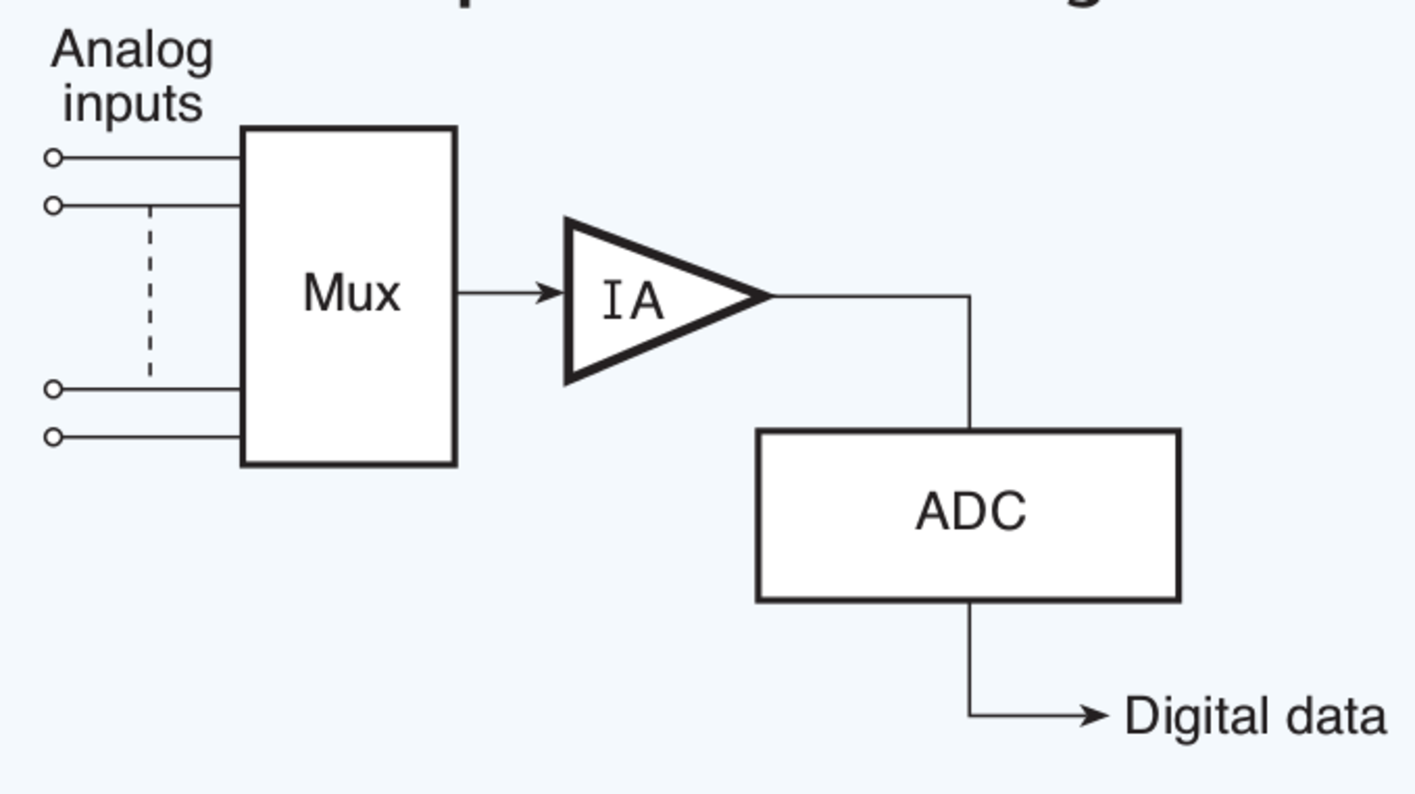
\includegraphics[width=\textwidth]{d2/daq_general}}
%\fbox{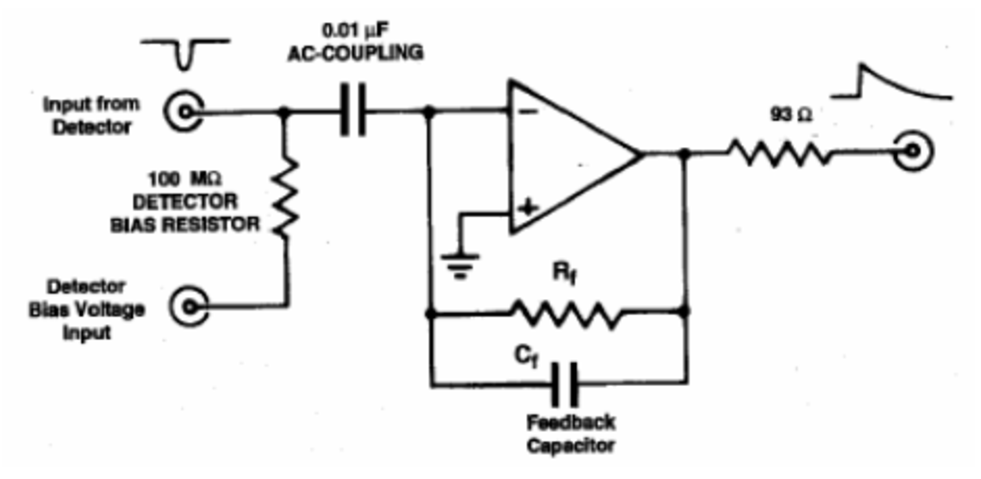
\includegraphics[width=\textwidth]{d2/typical_preamp}}
% \end{column}
%\end{columns}
%\end{frame} 
%
%\begin{frame}
%	\frametitle{Definiciones: ENOB}
%		\begin{block}{}
%    	\begin{itemize}
%      	\item Sistema todo-en-uno
%        \item Guardar los datos para futuros análisis (off-line data analysis)
%              en un lugar centralizado y de fácil acceso para toda la
%							Colaboración
%        \item Uniformizar el formato de los datos/archivos guardados
%    	\end{itemize}
%		\end{block}
%\end{frame} 
%------------------------------------------------------------------------------
\section{Procesamiento de señal}
%------------------------------------------------------------------------------

\begin{frame}
\frametitle{Procesamiento de señal}
\begin{center}
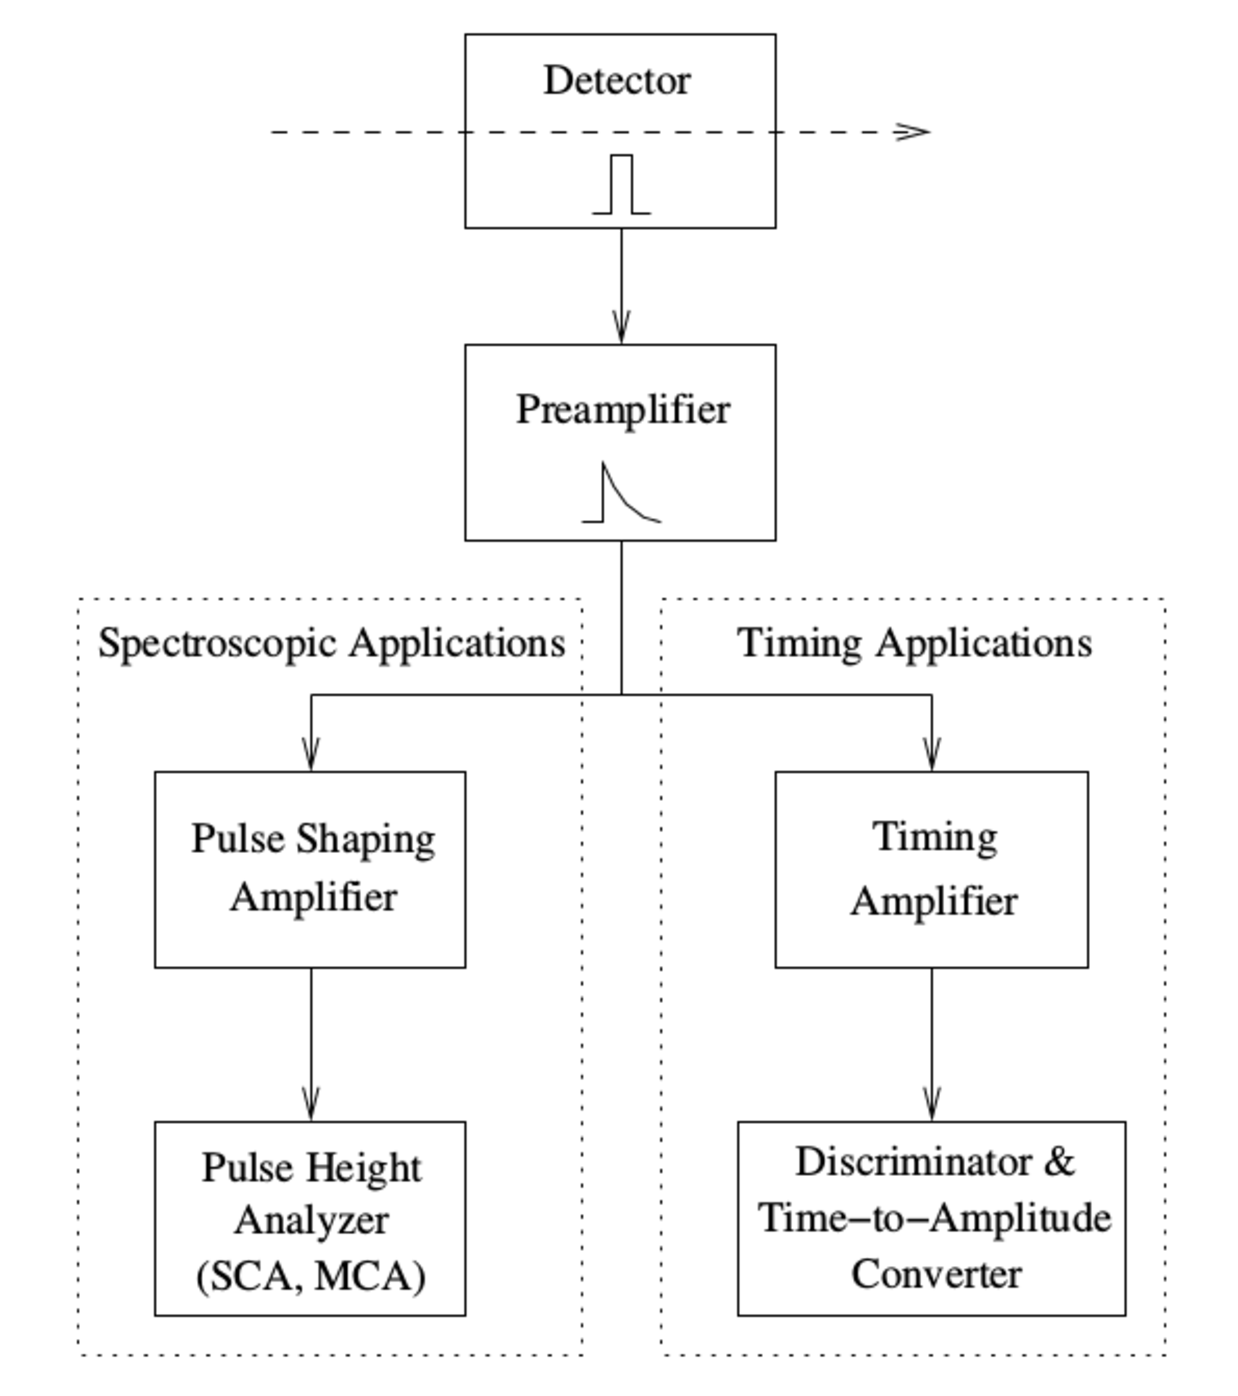
\includegraphics[width=.5\textwidth]{d2/typical_asp} 
\end{center}
\end{frame} 
%%---21/02
\begin{frame}
\frametitle{Procesamiento de señal}
Dos piezas de información son importantes con respecto a la detección y medición de radiación:
\begin{itemize}
\item amplitud $\rightarrow$ espectroscopia de energía
\item tiempos involucrados con los pulsos de salida $\rightarrow$ tracking de partículas
\end{itemize} 
\end{frame} 

%\begin{frame}
%\frametitle{Procesamiento de señal}
%Dos piezas de información son importantes con respecto a la detección y medición de radiación:
%\begin{itemize}
%\item amplitud $\rightarrow$ espectroscopia de energía
%\item tiempos involucrados con los pulsos de salida $\rightarrow$ tracking de partículas
%\end{itemize} 
%\begin{itemize}
%\item analógico 
%\item digital
%\end{itemize} 
%\end{frame} 

%%---
\begin{frame}
\frametitle{Procesamiento de señal}
\framesubtitle{{\color{blue}Clasificación}}
\begin{block}{}
Los detectores de radiación requieren electrónica de procesamiento de pulsos (o
señales) para que la información de energía y/o tiempo involucrada en las
interacciones pueda ser extraída apropiadamente
\end{block}
\begin{block}{}
Existen dos tipos de señal en las mediciones de radiación: pulsos
{\color{blue}lineales} y {\color{blue}lógicos}. 
\begin{itemize}
\item Un {\color{blue}pulso lineal} es una señal que transporta información a través de su
\alert{amplitud} y \alert{forma}
\item Un {\color{blue}pulso lógico} es una señal de tamaño y forma estándar que lleva
información sólo por su \alert{presencia} o \alert{ausencia}
\end{itemize}
\end{block}
\end{frame} 

\begin{frame}
\frametitle{Procesamiento de señal}
\framesubtitle{{\color{blue}Conformación de pulsos}}
\begin{center}
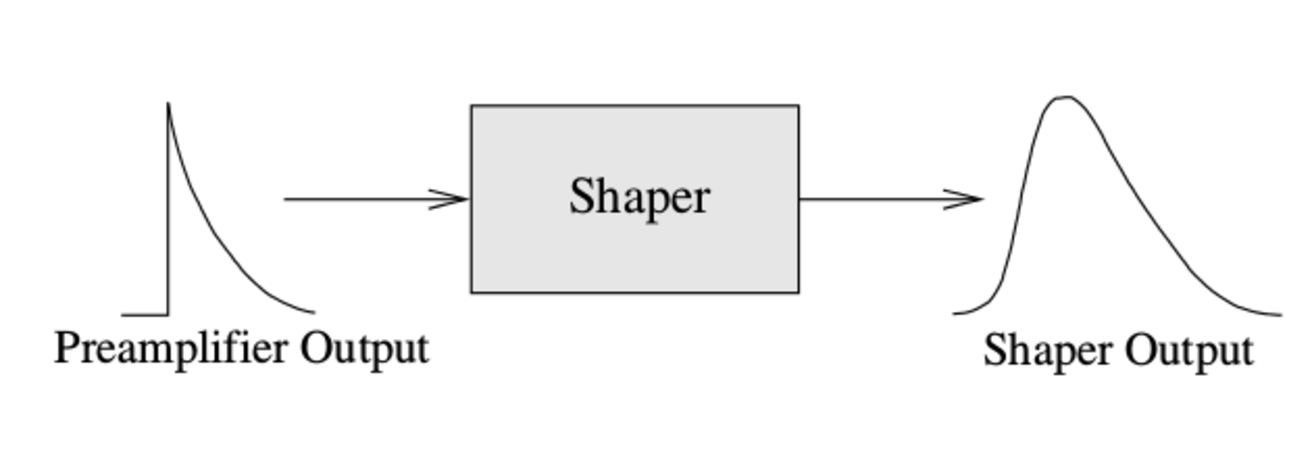
\includegraphics[width=.8\textwidth]{d2/pulse_shaper} 
\end{center}
%\vspace*{5mm}
\begin{block}{Conformación de pulsos}
\begin{itemize}
\item Carga en el pulso $\propto$ energía absorvida
\item Altura del pulso $\propto$ energía absorvida
\end{itemize}
\end{block}
\end{frame} 

\begin{frame}
\frametitle{Procesamiento de señal}
\framesubtitle{{\color{blue}Conformación de pulsos}}
\begin{itemize}
\item El pulso {\color{blue}más amplio} es necesario para {\color{blue}reducir el ruido} 
\item El \alert{pico redondeado} es necesario para \alert{medir la amplitud con precisión}
\item Puede haber pulsos unipolares o bipolares
\end{itemize}
Hay dos objetivos para transformar la señal del detector en un pulso bien definido:
\begin{itemize}
\item Incrementar la relación $S/N$ 
\item Incrementar la resolución de pares de pulsos
\end{itemize}
\begin{center}
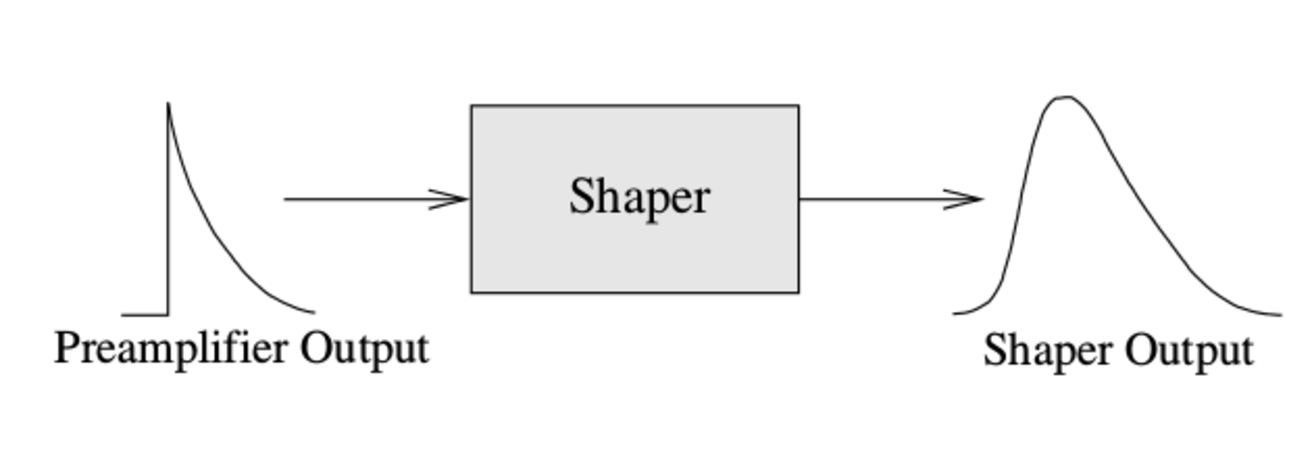
\includegraphics[width=.8\textwidth]{d2/pulse_shaper} 
\end{center}
\end{frame} 

\begin{frame}
\frametitle{Procesamiento de señal}
\framesubtitle{Filtrado y conformación (shaping)}
\begin{center}
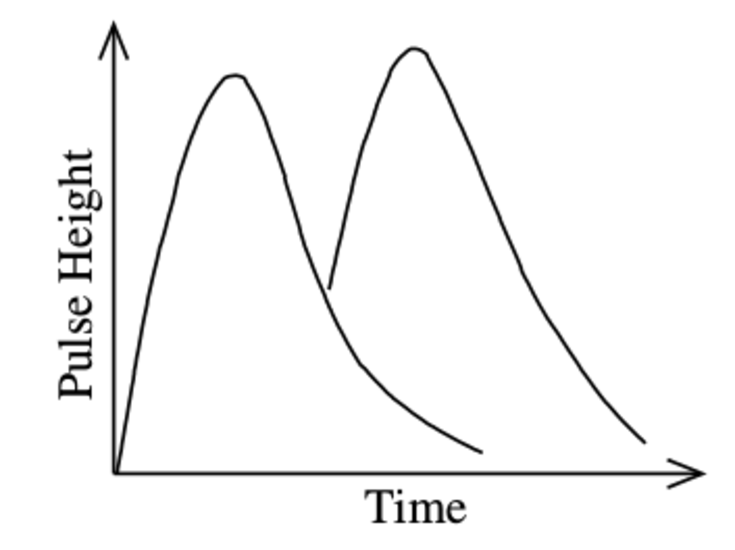
\includegraphics[width=.4\textwidth]{d2/pileup_not_corrected} 
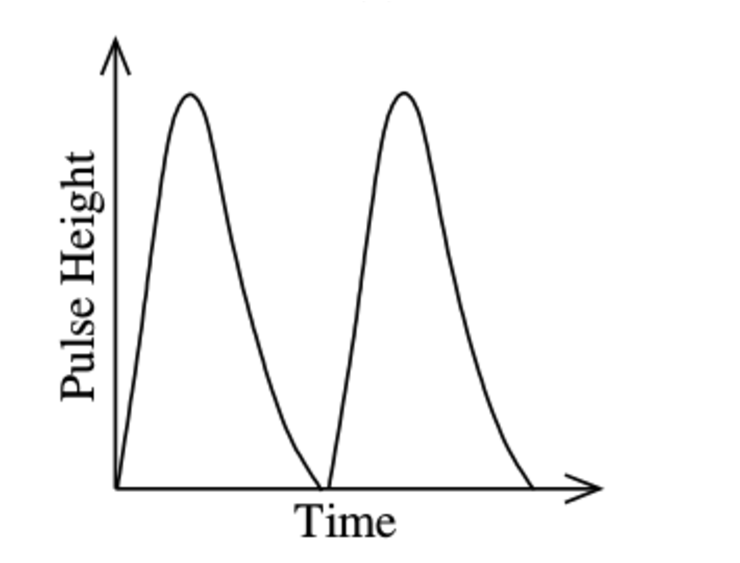
\includegraphics[width=.4\textwidth]{d2/pileup_corrected} 
\end{center}

En mediciones de alta velocidad de conteo, a veces se desea acortar la duración 
del pulso para evitar acumulaciones ({\color{blue}pile-up})

Básicamente, existen dos métodos para llevar a cabo esta tarea:
\begin{itemize}
\item Circuito diferenciador $CR$ o filtro pasa-altos
\item Circuito integrador $RC$ o filtro pasa-bajos
\end{itemize}
\end{frame}

\begin{frame}
\frametitle{Filtrado y conformación (shaping)}
\framesubtitle{{\color{blue}Circuito diferenciador $CR$ o filtro pasa-altos}}
\begin{center}
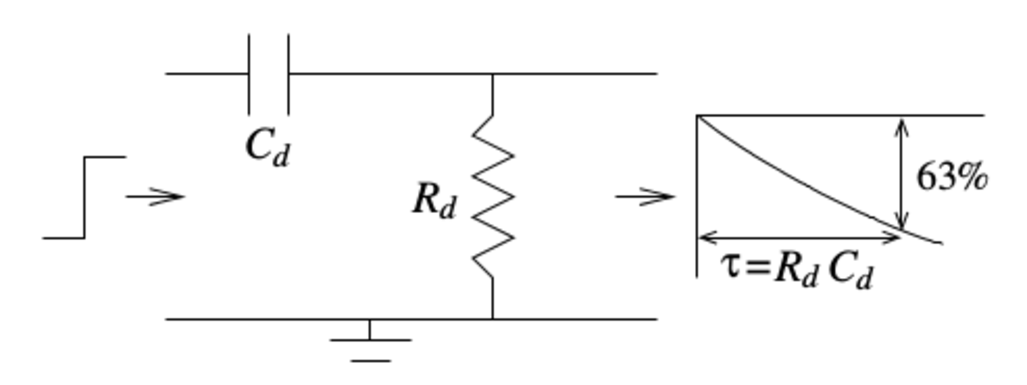
\includegraphics[width=0.8\textwidth]{d2/cr_differentiator2}
\end{center}
Este circuito atenúa las frecuencias $f \leq \frac{1}{2\pi R_dC_d}$
\begin{itemize}
\item \alert{La parte plana del pulso se degrada y decae hacia la línea de base, 
acortando el pulso}
\item \alert{La parte rápida del pulso (flanco de subida), que depende de las 
frecuencias altas, no se ve afectada}
\end{itemize}
\end{frame}

\begin{frame}
\frametitle{Filtrado y conformación (shaping)}
\framesubtitle{{\color{blue}Circuito diferenciador $CR$ o filtro pasa-altos}}
\begin{center}
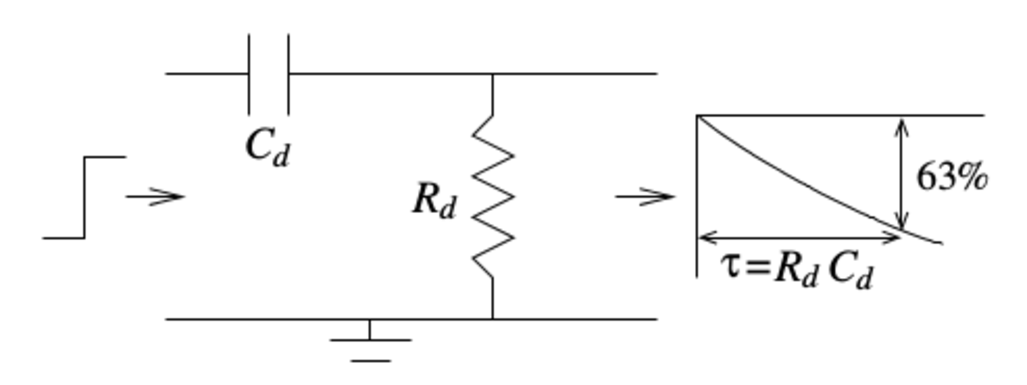
\includegraphics[width=0.8\textwidth]{d2/cr_differentiator2}
\end{center}
$$\tau_d = R_d C_d$$
%$$V_{out} \approx e^{-t/\tau_d} \qquad \tau_d = R_d C_d$$

\begin{alertblock}{}
Si $\tau_d < t_r$ el pulso diferenciado empieza a decaer antes de alcanzar su 
máxima amplitud $\rightarrow$ \alert{déficit balístico}
\end{alertblock}
\end{frame}

\begin{frame}
\frametitle{Filtrado y conformación (shaping)}
\framesubtitle{{\color{blue}Circuito diferenciador $CR$ o filtro pasa-altos}}
\begin{center}
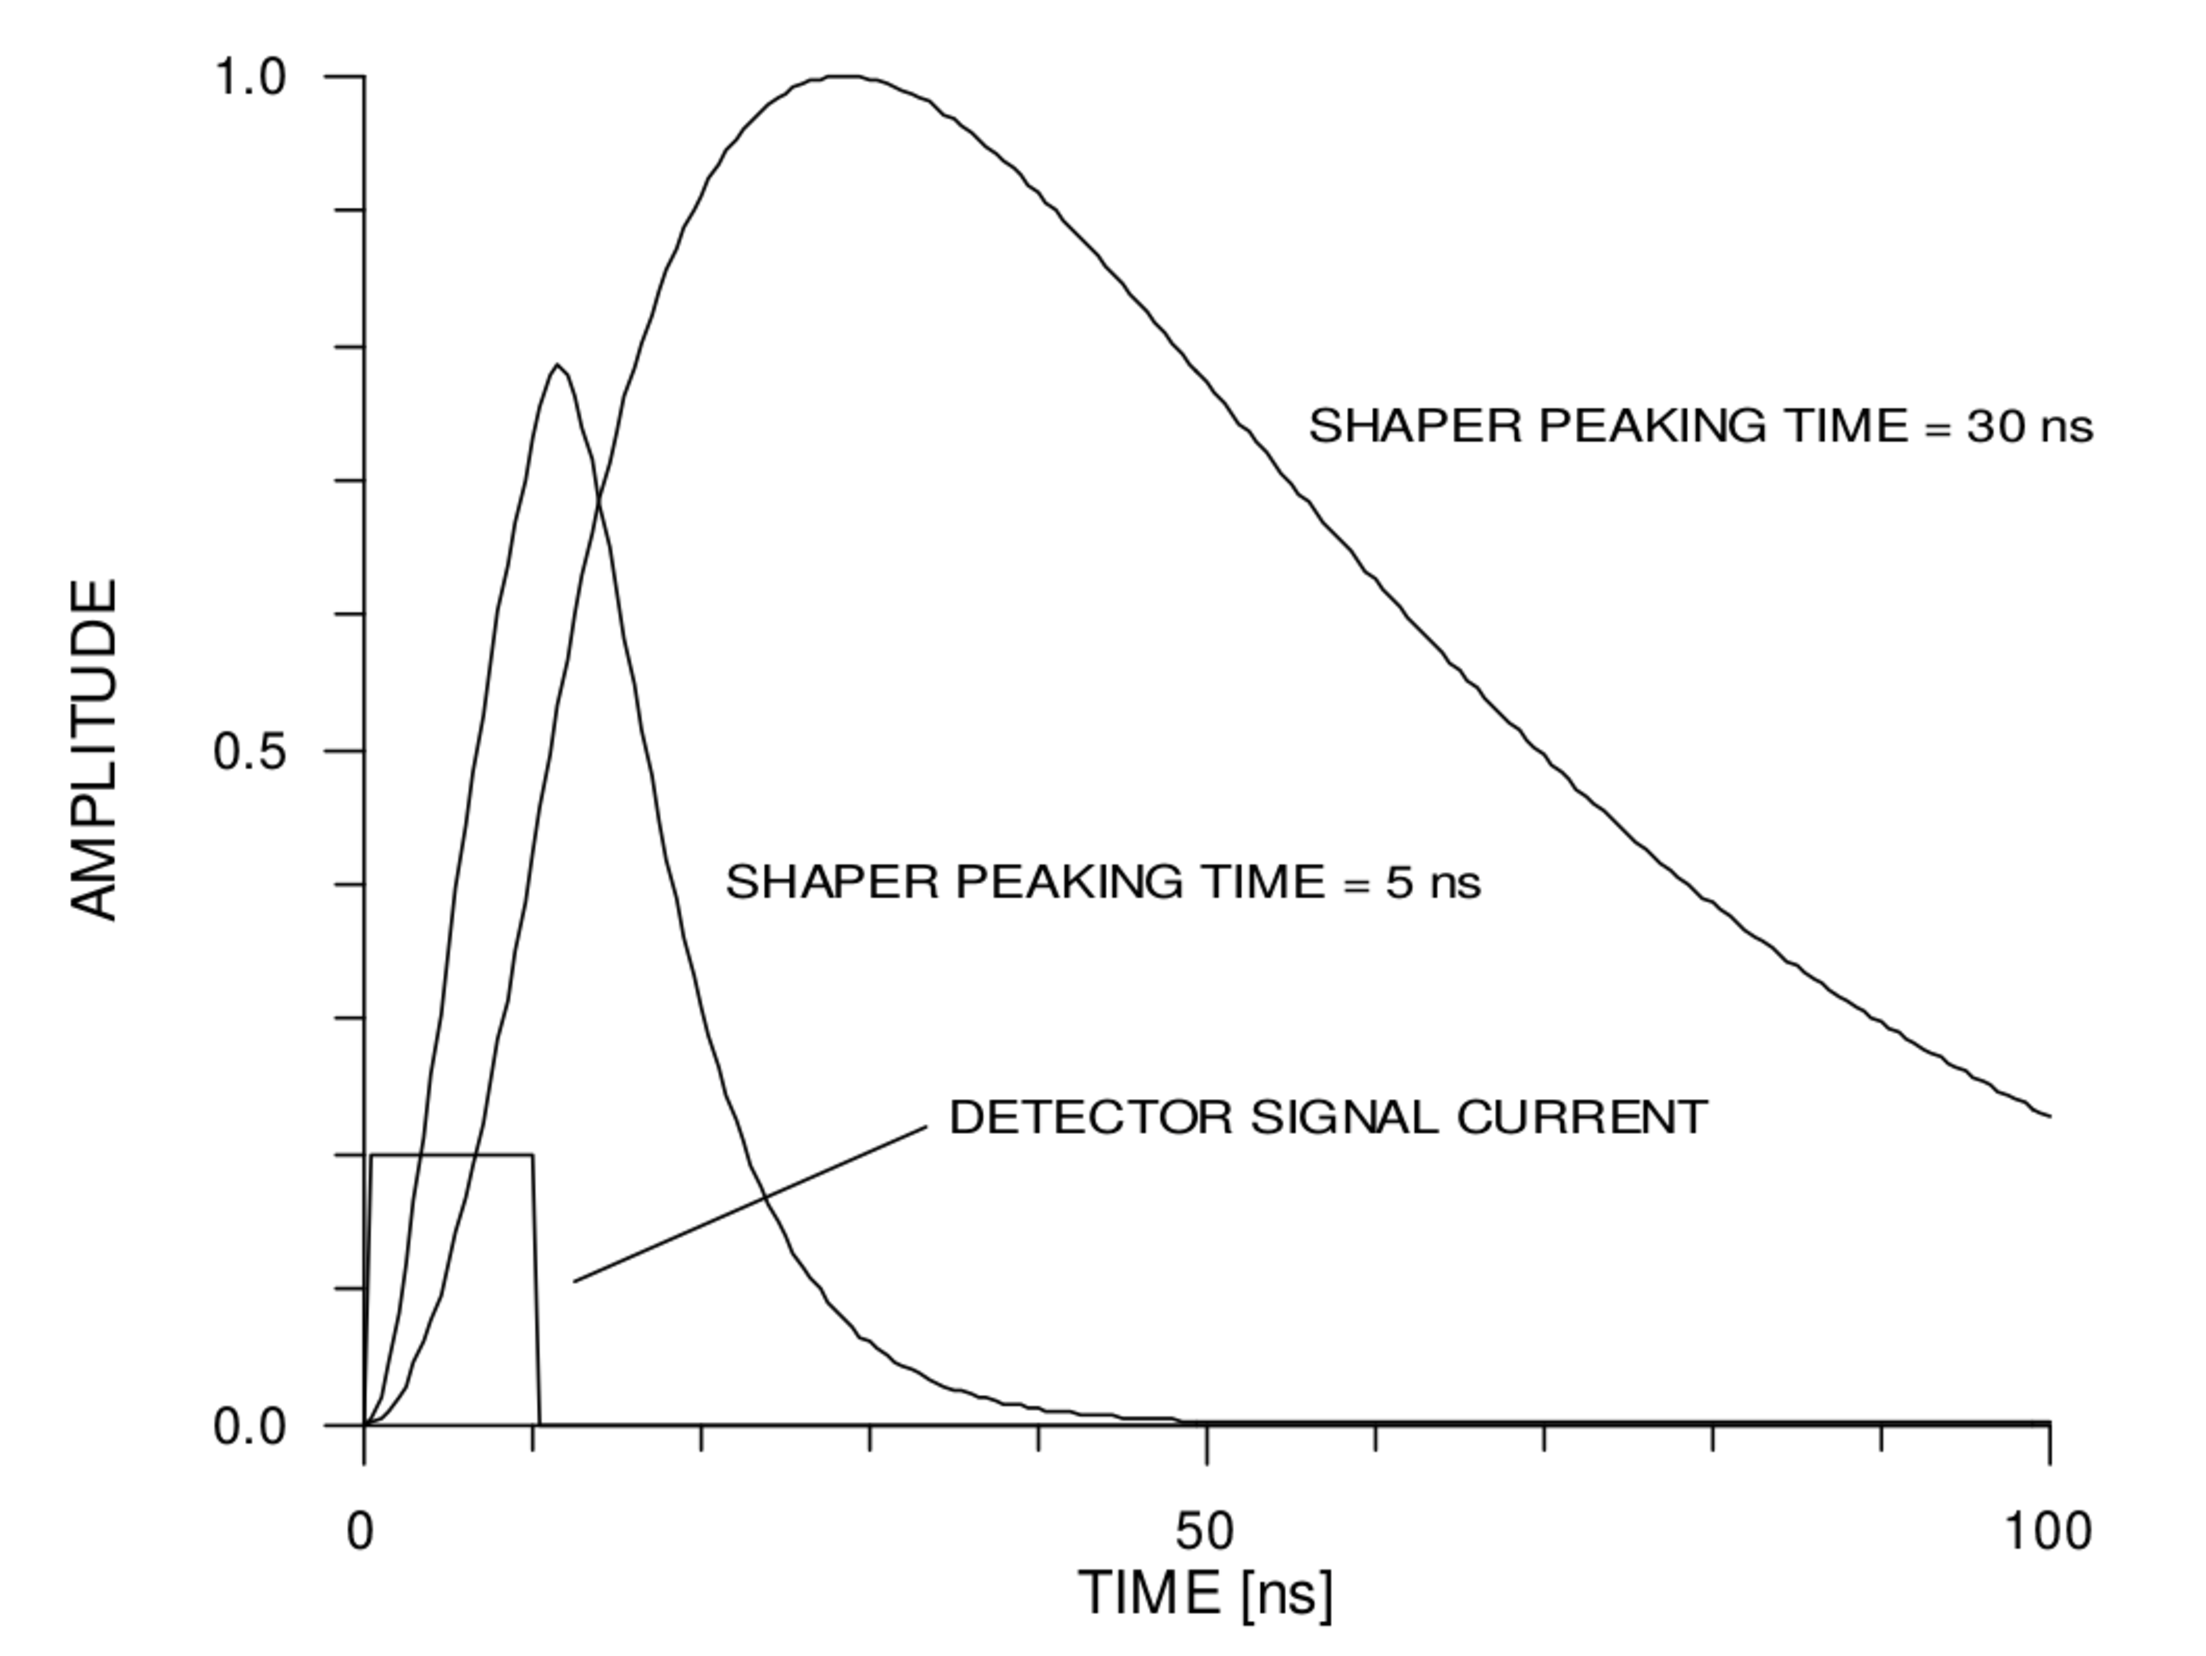
\includegraphics[width=0.8\textwidth]{d2/deficit_balistico}
\end{center}
\end{frame}

\begin{frame}
\frametitle{Filtrado y conformación (shaping)}
\framesubtitle{{\color{blue}Circuito diferenciador $CR$ o filtro pasa-altos}}
\begin{columns}
\begin{column}{0.5\textwidth}
\begin{center}
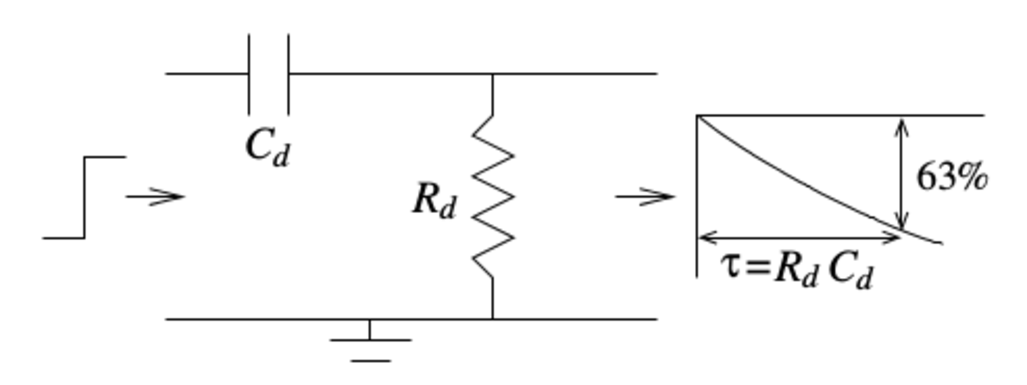
\includegraphics[width=\textwidth]{d2/cr_differentiator2}
\end{center}
\end{column}
\begin{column}{0.5\textwidth}
$$V_{in} = \frac{Q}{C} + V_{out}$$
$$\frac{dV_{in}}{dt} = \frac{1}{C}\frac{dQ}{dt} + \frac{dV_{out}}{dt}$$
$$\frac{dQ}{dt} = i = \frac{V_{out}}{R}$$
$${\color{violet}\frac{dV_{in}}{dt} = \frac{1}{RC}V_{out} + \frac{dV_{out}}{dt}}$$
\end{column}
\end{columns}
\begin{alertblock}{}
Si $\tau_d$ es pequeño:
$\frac{dV_{in}}{dt} \approx \frac{1}{\tau_d}\,V_{out} \rightarrow
{\color{blue}V_{out} \approx e^{-t/\tau_d}}$

\vspace{2mm}
Si $\tau_d$ es grande:
$\frac{dV_{in}}{dt} \approx \frac{dV_{out}}{dt} \rightarrow {\color{blue}V_{out} \approx
V_{in}}$
\end{alertblock}
\alert{El circuito diferenciará el pulso de entrada sólo si $\tau_d$ es pequeño 
comparado con el ancho del pulso}
\end{frame}

\begin{frame}
\frametitle{Filtrado y conformación (shaping)}
\framesubtitle{{\color{blue}Circuito integrador $RC$ o filtro pasa-bajos}}
\begin{center}
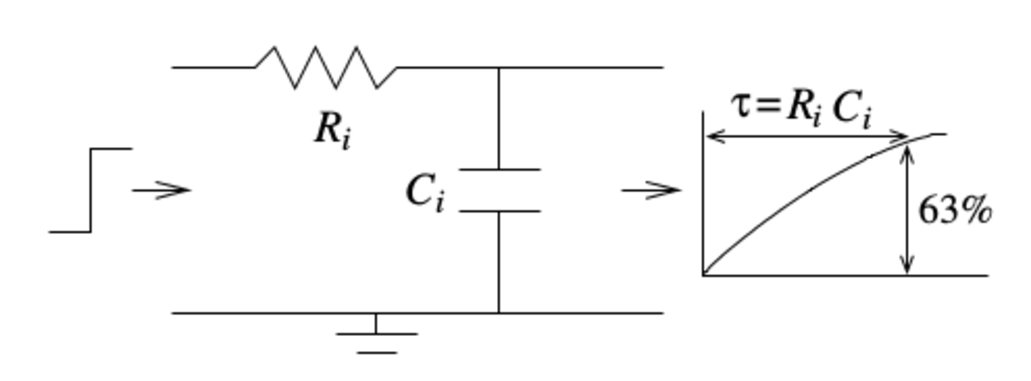
\includegraphics[width=0.8\textwidth]{d2/rc_integrator2}
\end{center}
Este circuito atenúa las frecuencias $f \geq \frac{1}{2\pi R_iC_i} \rightarrow \tau_i = R_iC_i$
\begin{itemize}
\item \alert{Afecta la subida rápida de los pulsos de entrada}
\item \alert{El pulso de salida se acerca exponencialmente hacia el máximo}
\end{itemize}
\end{frame}

\begin{frame}
\frametitle{Filtrado y conformación (shaping)}
\framesubtitle{{\color{blue}Circuito integrador $RC$ o filtro pasa-bajos}}
\begin{center}
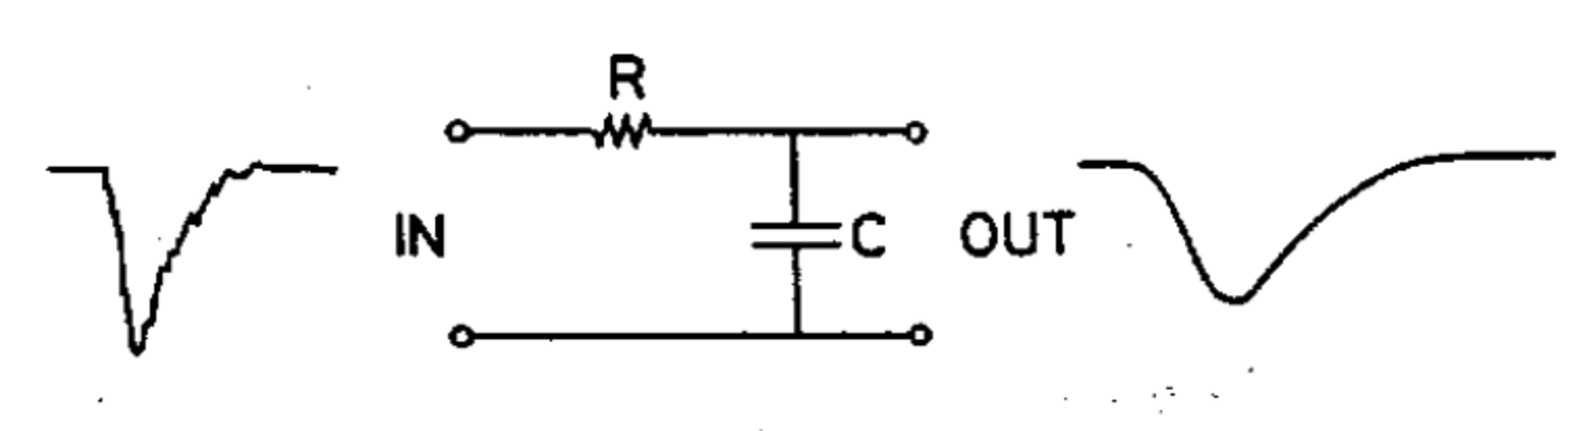
\includegraphics[width=0.8\textwidth]{d2/filtrado_por_integracion}
\end{center}
El uso principal de este circuito es el de {\color{blue}suavizado de señales ruidosas} 
\end{frame}

\begin{frame}
\frametitle{Filtrado y conformación (shaping)}
\framesubtitle{{\color{blue}Circuito integrador $RC$ o filtro pasa-bajos}}
\begin{columns}
\begin{column}{0.5\textwidth}
\begin{center}
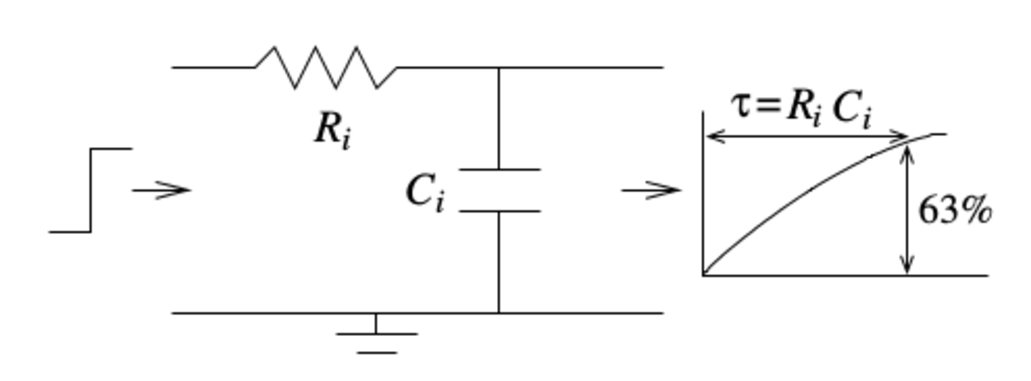
\includegraphics[width=\textwidth]{d2/rc_integrator2}
\end{center}
\end{column}
\begin{column}{0.5\textwidth}
$$V_{in} = iR + V_{out}$$
$$i = \frac{dQ}{dt} = C\frac{dV_{out}}{dt}$$
$${\color{violet}V_{in} = RC\frac{dV_{out}}{dt} + V_{out}}$$
\end{column}
\end{columns}
\begin{alertblock}{}
Si $\tau_i$ es pequeño:
${\color{blue}V_{out} \approx V_{in}}$

\vspace{2mm}
Si $\tau_i$ es grande:
$V_{in} \approx \tau_i\,\frac{dV_{out}}{dt} \rightarrow {\color{blue}V_{out}
\approx 1 - e^{-t/\tau_i}} $
\end{alertblock}
\alert{El circuito integrará el pulso de entrada sólo si $\tau_i$ es grande 
comparado con el ancho del pulso}
\end{frame}

\begin{frame}
\frametitle{Filtrado y conformación (shaping)}
\framesubtitle{{\color{blue}Shaping CR-RC}}
\begin{center}
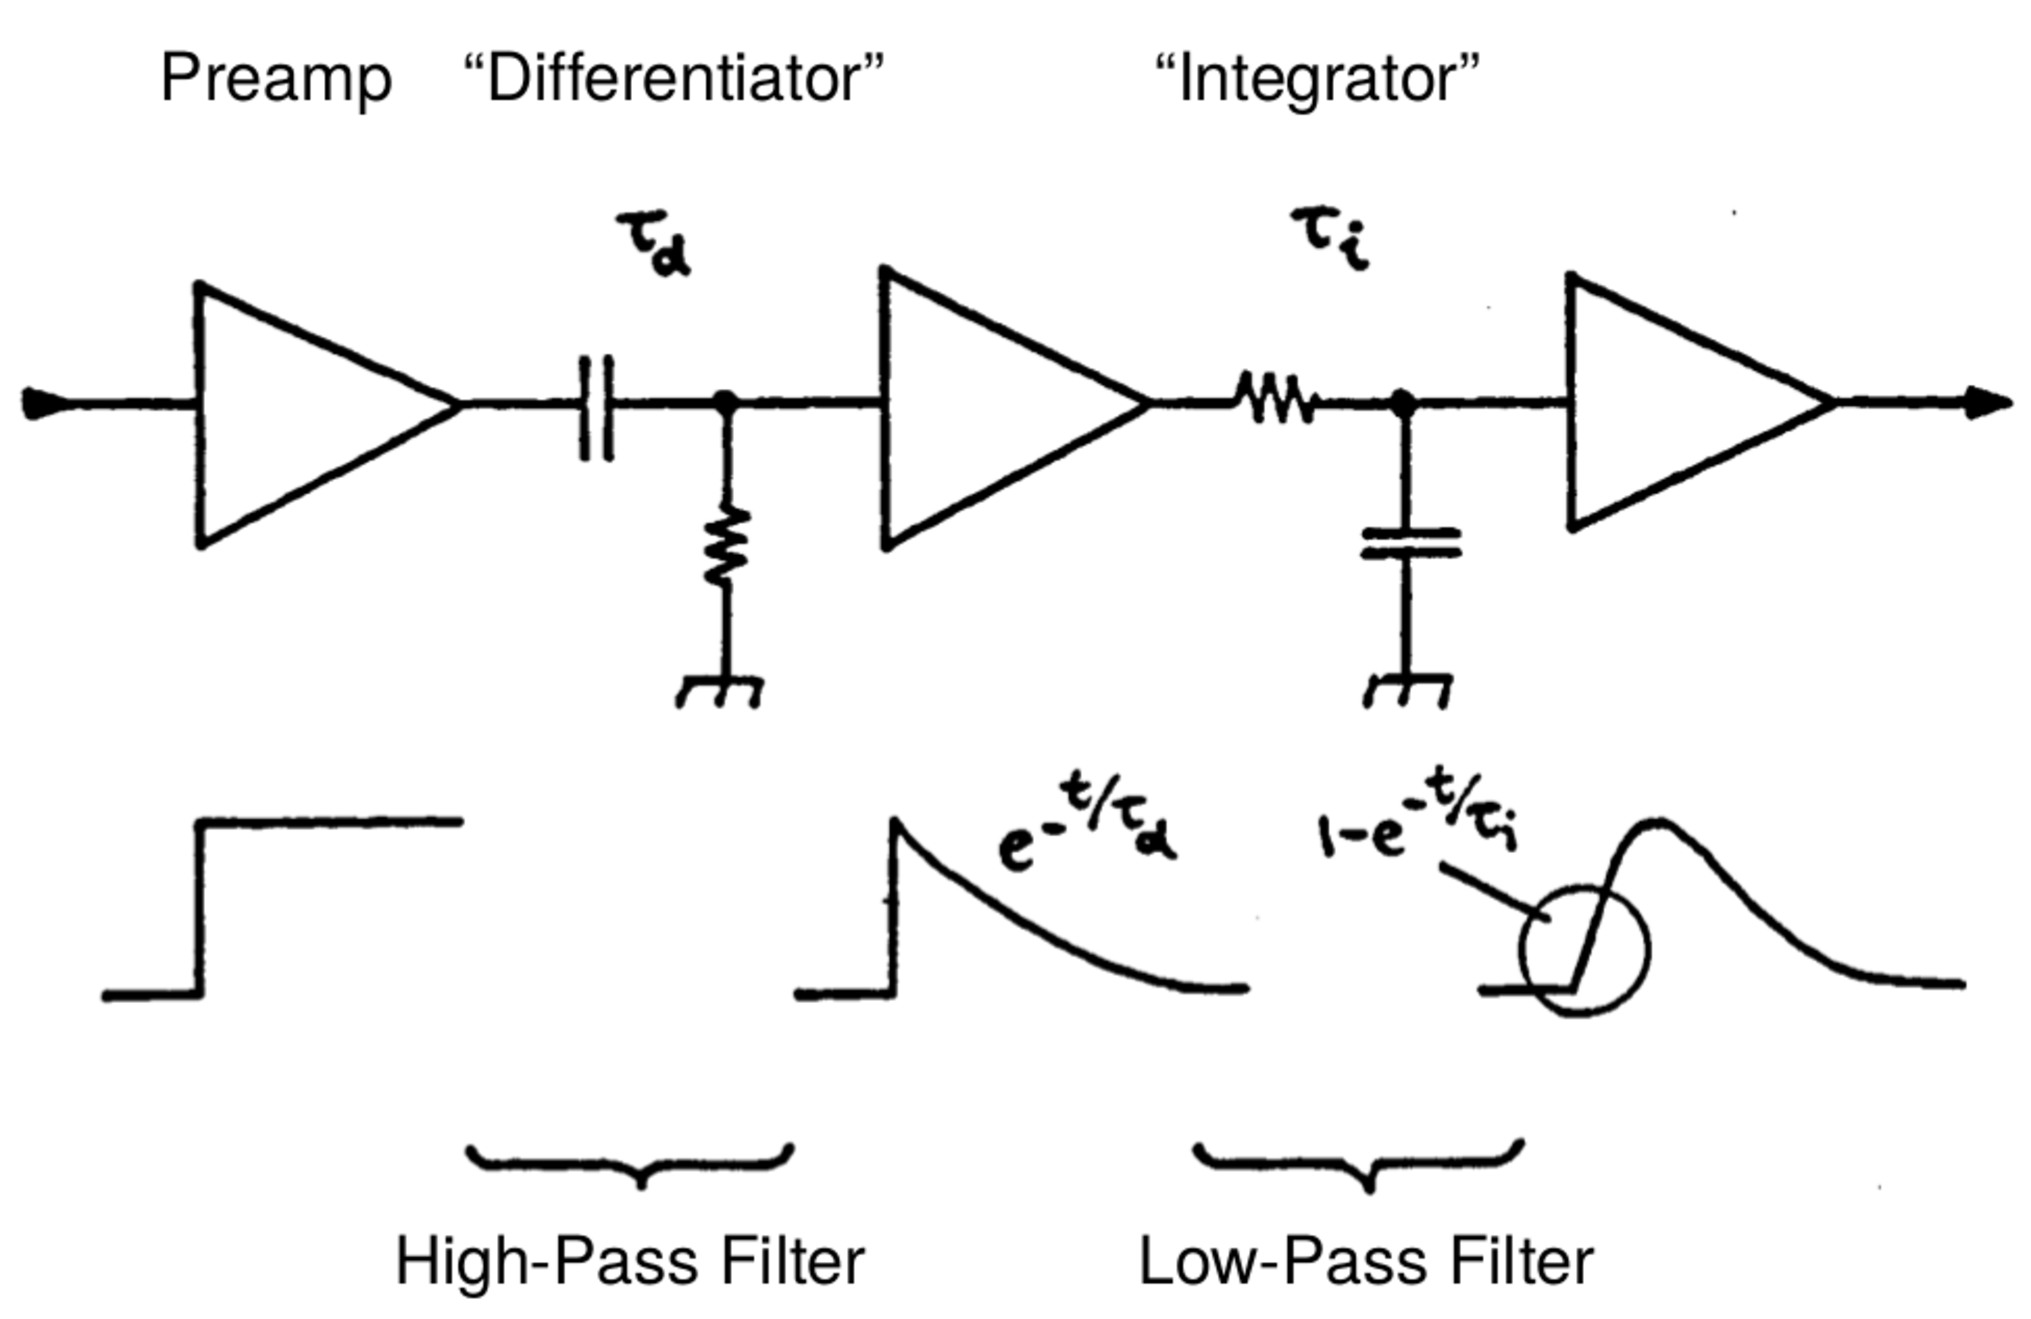
\includegraphics[width=0.75\textwidth]{d2/cr_rc_shaping2}
\end{center}
\begin{itemize}
\item Arreglo simple: comportamiento frente al ruido sólo 36\% peor que uun
filtro óptimo con las mismas constantes 
\end{itemize}
\end{frame}

\begin{frame}
\frametitle{Filtrado y conformación (shaping)}
\framesubtitle{{\color{blue}Shaping CR-RC}}
\begin{columns}
\begin{column}{0.5\textwidth}
\begin{itemize}
\item Quizá el método más simple y más usado para el conformació de pulsos
\item Dos partes: un diferenciador CR y un integrador RC
\item El perfil del pulso, luego de pasar por este shaper es
$$V_{out} = \frac{\tau_d(\tau_d e^{-t/\tau_d} + \tau_i e^{-t/\tau_i})}{\tau_d
\tau_i(\tau_d - \tau_i)}$$
\end{itemize}
\end{column}
\begin{column}{0.5\textwidth}
\begin{center}
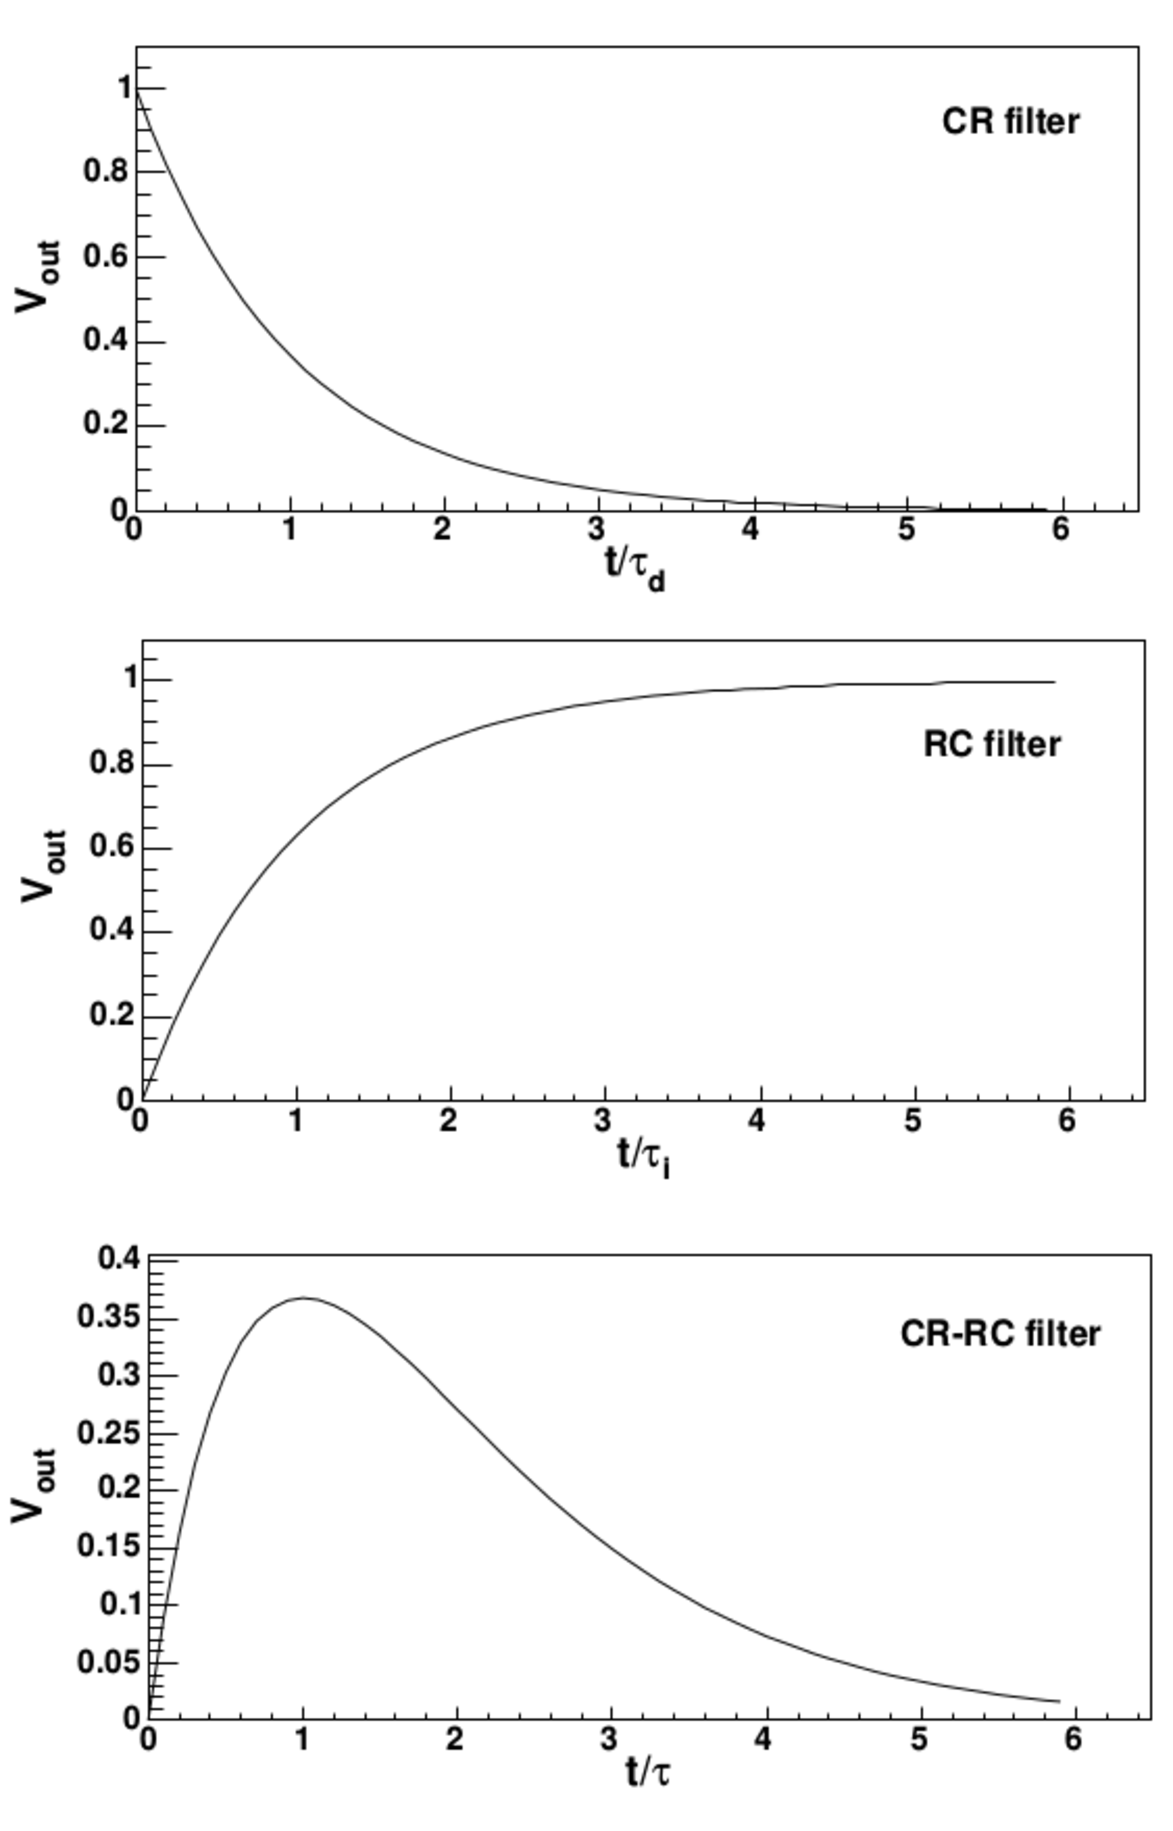
\includegraphics[width=0.75\textwidth]{d2/cr_rc_shaping}
\end{center}
\end{column}
\end{columns}
\end{frame}

\begin{frame}
\frametitle{Filtrado y conformación (shaping)}
\framesubtitle{{\color{blue}Shaping CR-RC}}
\begin{itemize}
\item Entonces el pulso de salida depende de las constantes de tiempo CR y RC
\item Generalmente se los elige de forma tal que se obtinen pulsos con un pico
redondeado, un tiempo de subida rápido y un tiempo de bajada largo
\item Para asegurar esto, se elije $\tau_d = \tau_i = \tau$, con lo cual
$$V_{out} = \frac{t}{\tau}e^{-t/\tau} $$
\end{itemize}
\end{frame}

\begin{frame}
\frametitle{Filtrado y conformación (shaping)}
\framesubtitle{{\color{blue}Shaping CR-RC}}
\begin{columns}
\begin{column}{0.5\textwidth}
\begin{itemize}
\item Respuesta a pulsos distintos 
\item Un pulso ``step''
\item Un pulso más realista, salido de un preamp. Notar la aparición de un
undershoot en este caso.
\end{itemize}
\end{column}
\begin{column}{0.5\textwidth}
\begin{center}
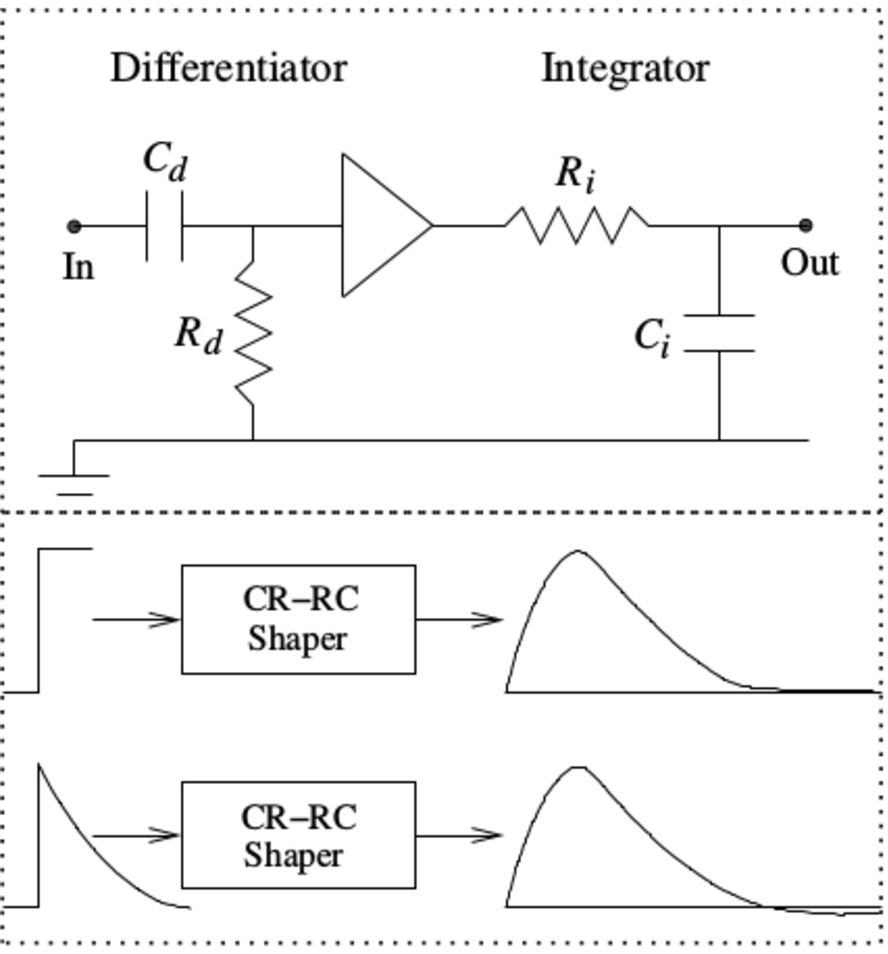
\includegraphics[width=0.85\textwidth]{d2/cr_rc_shaping_amp}
\end{center}
\end{column}
\end{columns}
\end{frame}

\begin{frame}
\frametitle{Filtrado y conformación (shaping)}
\framesubtitle{{\color{blue}Shaping CR-RC}}
\begin{itemize}
\item La elección de las constantes de tiempo CR-RC depende de la aplicación
particular
\item La resolución en la medición y la capacidad de conteo rápido son dos
factores que compiten para obtener una solución {\color{blue}óptima} 
\item Si llegan una gran cantidad de pulsos durante el tiempo de un undershoot,
las amplitudes medidas van a estar alejadas del valor real 
\item Para resolver este tipo de problemas, existe lo que se conoce como
{\color{blue}cancelación polo-cero}
\end{itemize}
\end{frame}

\begin{frame}
\frametitle{Filtrado y conformación (shaping)}
\framesubtitle{{\color{blue}Efecto de las constantes relativas}}
\begin{center}
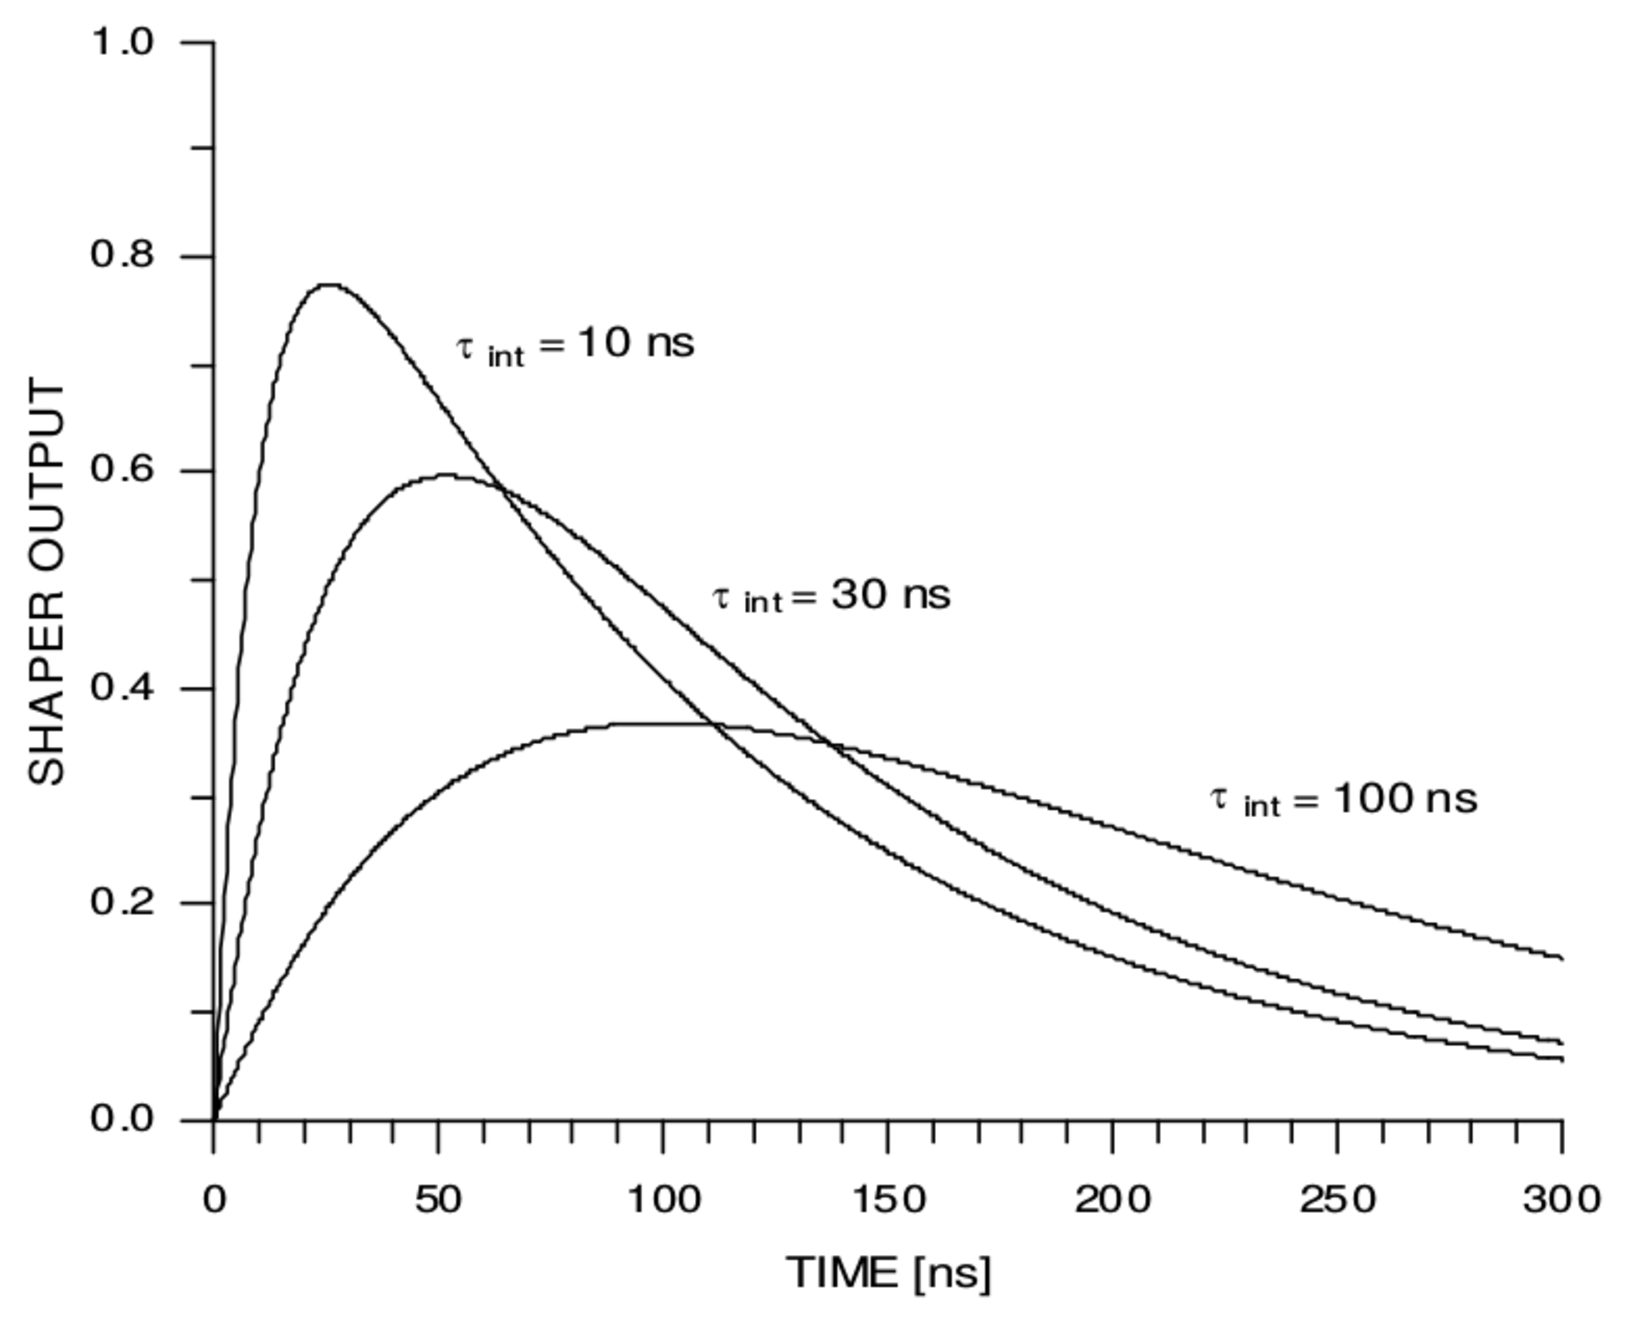
\includegraphics[width=0.5\textwidth]{d2/efecto_tc_shaping}
\end{center}
\begin{itemize}
\item Consideremos un shaper CR-RC con $\tau_d = 100\,ns$ (fijo)
\item Incrementar $\tau_i$ baja la freceuncia de corte más alta, lo cual
decrementa el ruido total a la salida.
\item Sin embargo, el pico de la señal también disminuye
\end{itemize}
\end{frame}

\begin{frame}
\frametitle{Filtrado y conformación (shaping)}
\framesubtitle{{\color{blue}Efecto de las constantes relativas}}
\begin{center}
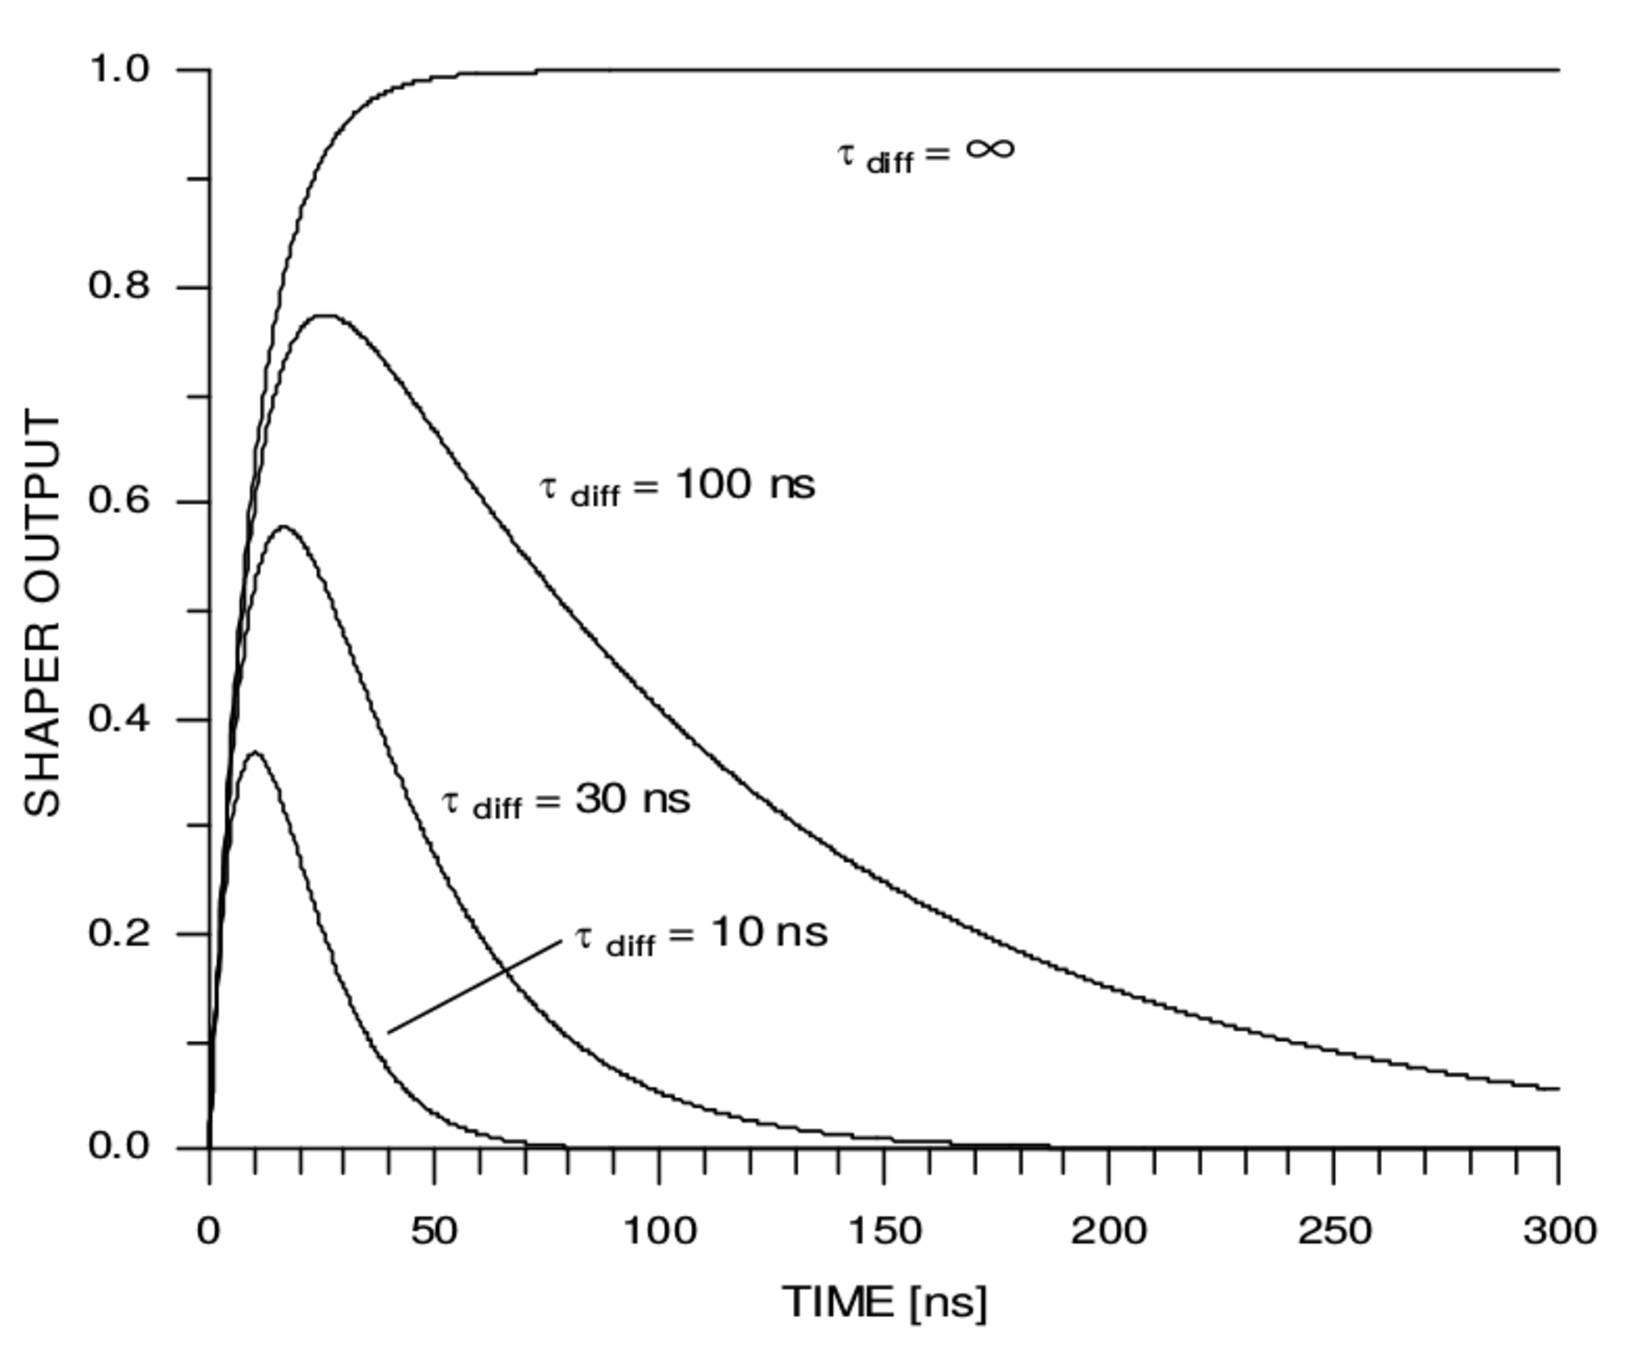
\includegraphics[width=0.5\textwidth]{d2/efecto_tc_shaper2}
\end{center}
\begin{itemize}
\item Consideremos ahora un shaper CR-RC con $\tau_i = 10\,ns$ (fijo)
\item Si $\tau_d$ se reduce, la amplitud de pico a la salida del
shaper se reduce
\item Notar que la necesida de limitar el ancho del pulso nos lleva a una
reducción significante en la señal de salida 
\end{itemize}
\end{frame}

\begin{frame}
\frametitle{Filtrado y conformación (shaping)}
\framesubtitle{{\color{blue}Resumen}}
\begin{itemize}
\item Para evaluar el comportamiento del shaper en cuanto a ruido sólo el
espectro de ruido es inadecuado
\item También se deben considerar los efectos sobre la señal
\item La amplitud de la señal también se ve afectada por la relación entre los
tiempos característicos del shaping y la duración de la señal  
\item Si el peaking time del shaper $<$ tiempo de colección del detector
$\implies$ pérdida de señal (pérdida balística)
\end{itemize}
\end{frame}

\subsection{Otros aspectos de la conformación de pulsos}

\begin{frame}
\frametitle{Otros aspectos de la conformación de pulsos}
\framesubtitle{Restauración de la línea de base}
En un sistema, un capacitor en serie previene la transmisión de componentes DC.

Una secuencia de pulsos unipolares tiene una componente DC que depende del
factor de trabajo, es decir, la tasa de eventos.

$\implies$ {\color{blue}La línea de base cambia para hacer que la carga global
transmitida sea igual a cero}
\begin{center}
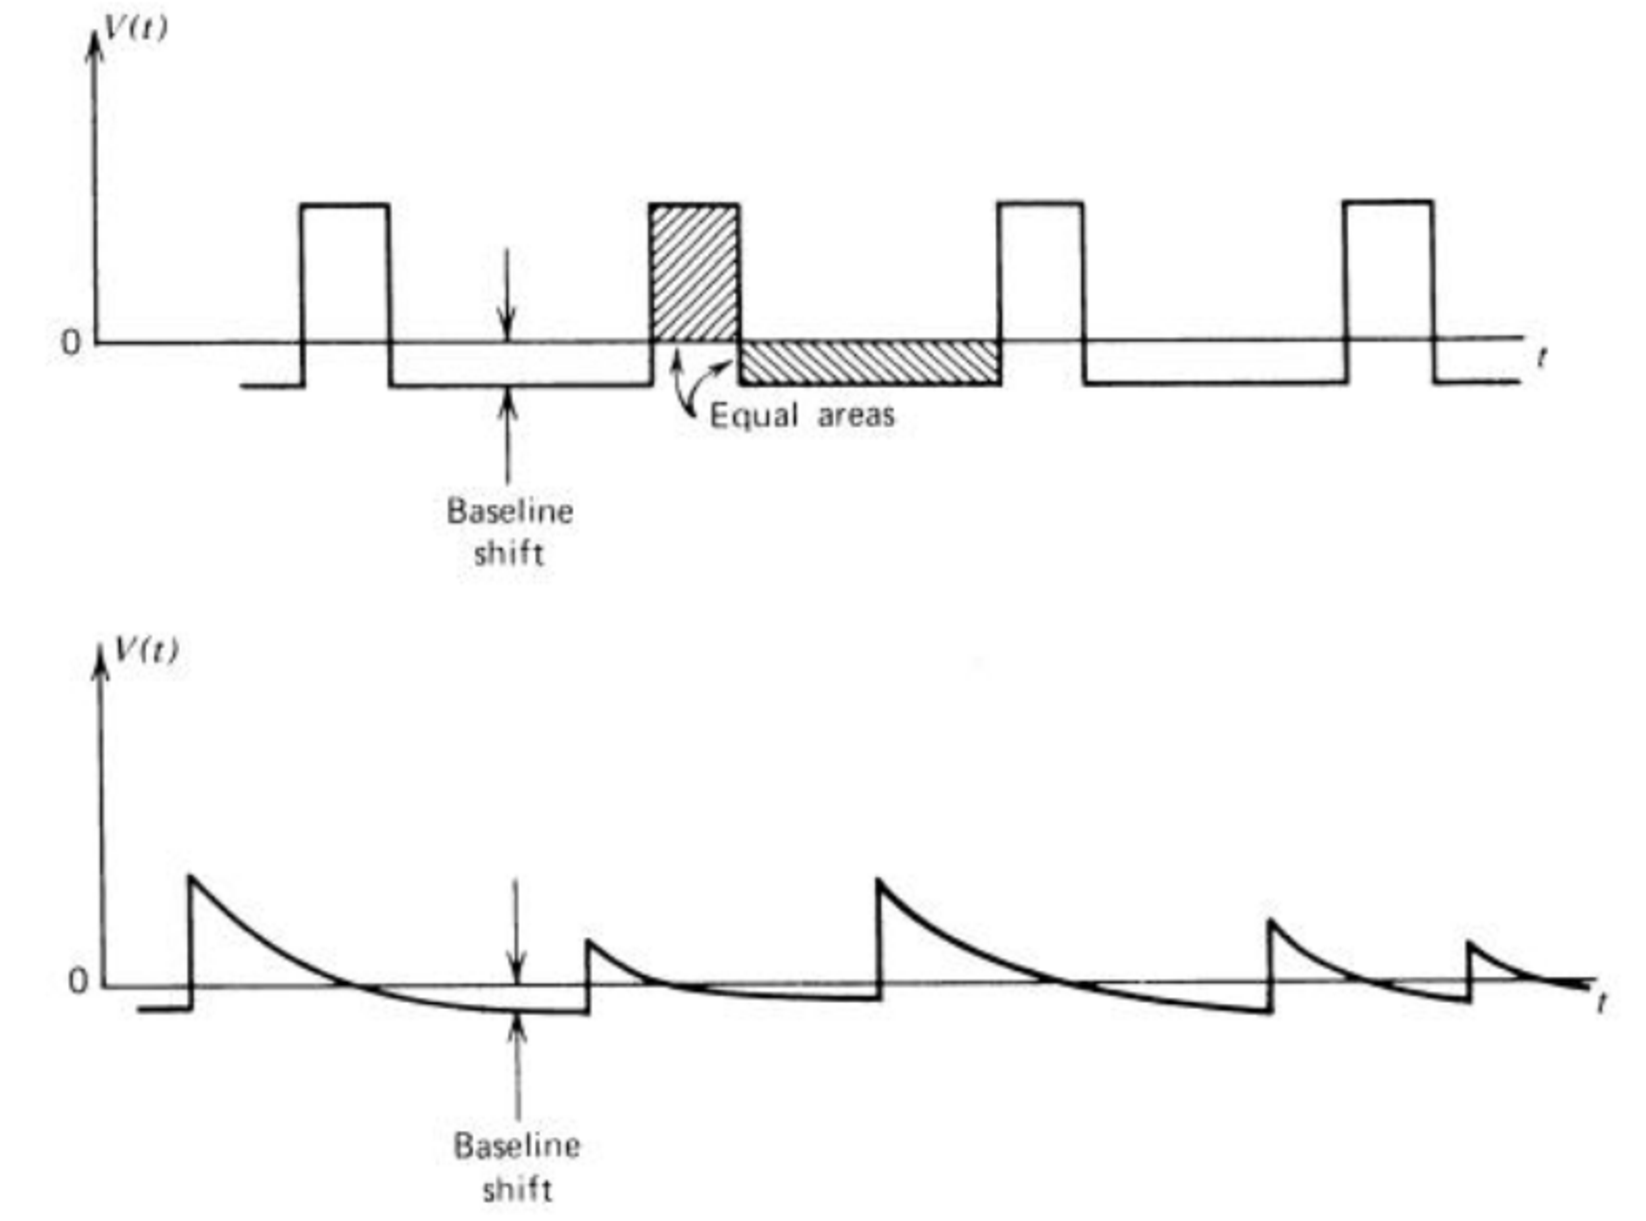
\includegraphics[width=0.5\textwidth]{d2/baseline_shift2}
\end{center}
\end{frame} 

\begin{frame}
\frametitle{Otros aspectos de la conformación de pulsos}
\framesubtitle{Restauración de la línea de base}
Tasas de eventos aleatorias $\implies$ fluctuaciones aleatorias del cambio de
línea de base $\implies$ {\color{blue}ensanchamiento espectral}
%\begin{itemize}
%\item Estos cambios ocurren siempre que la $G_{DC} \neq G_{BW}$ 
%\end{itemize}

Este efecto se puede mitigar con el uso de un restaurador de línea de base (BLR).
\begin{columns}
\begin{column}{0.5\textwidth}
\begin{center}
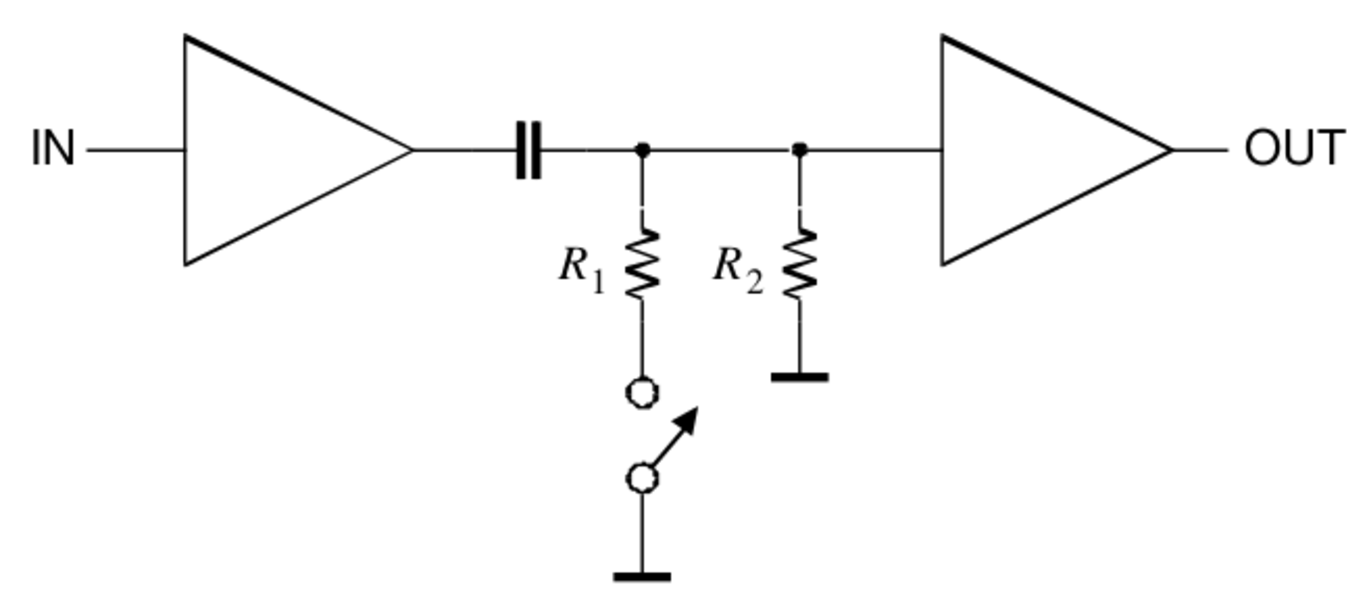
\includegraphics[width=\textwidth]{d2/circuito_blr}
\end{center}
\end{column}
\begin{column}{0.5\textwidth}
\begin{alertblock}{Principio del BLR}
Conectar la línea de señal a tierra durante la ausencia señal para establecer la
línea de base justo antes de la llegada de un pulso
\end{alertblock}
\end{column}
\end{columns}
$R_1$ y $R_2$ determinan las constantes de tiempo de carga y descarga.

La constante de tiempo de descarga (interruptor abierto) debe ser mucho mayor
que el ancho del pulso.

\alert{Esencial} $\rightarrow$ buena compensación polo-cero para restauración de linea de base 
adecuada
\end{frame} 

\begin{frame}
\frametitle{Otros aspectos de la conformación de pulsos}
\framesubtitle{Compensación polo-cero}
\begin{center}
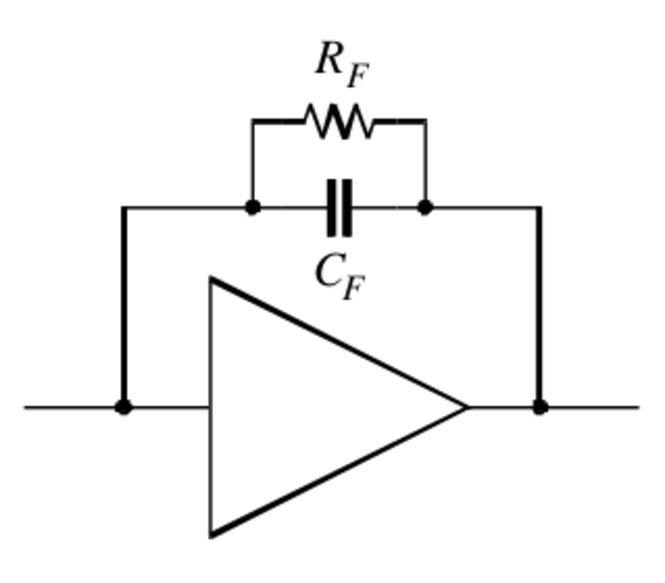
\includegraphics[width=0.4\textwidth]{d2/pz_csp}
\end{center}
El capacitor de realimentación en el preamp sensible a carga debe descargarse. 
Comúnmente se hace con una resistencia en paralelo.
\end{frame} 

\begin{frame}
\frametitle{Otros aspectos de la conformación de pulsos}
\framesubtitle{Compensación polo-cero}
\begin{columns}
\begin{column}{0.6\textwidth}
La salida ya no es un escalón, sino que disminuye exponencialmente

Decaimiento exponencial superpuesto a la salida del conformador
\begin{itemize}
\item[$\implies$] Undershoot
\item[$\implies$] Pérdida de resolución debido a variación de la línea de base
\end{itemize}
Agregar $R_{pz}$ al diferenciador
\begin{center}
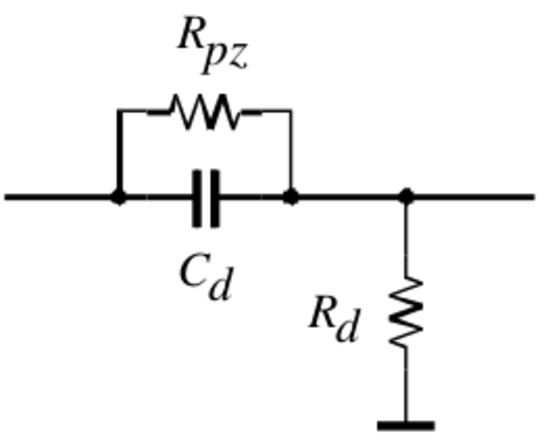
\includegraphics[width=0.4\textwidth]{d2/rpz_added}
\end{center}
\end{column}
\begin{column}{0.4\textwidth}
\begin{center}
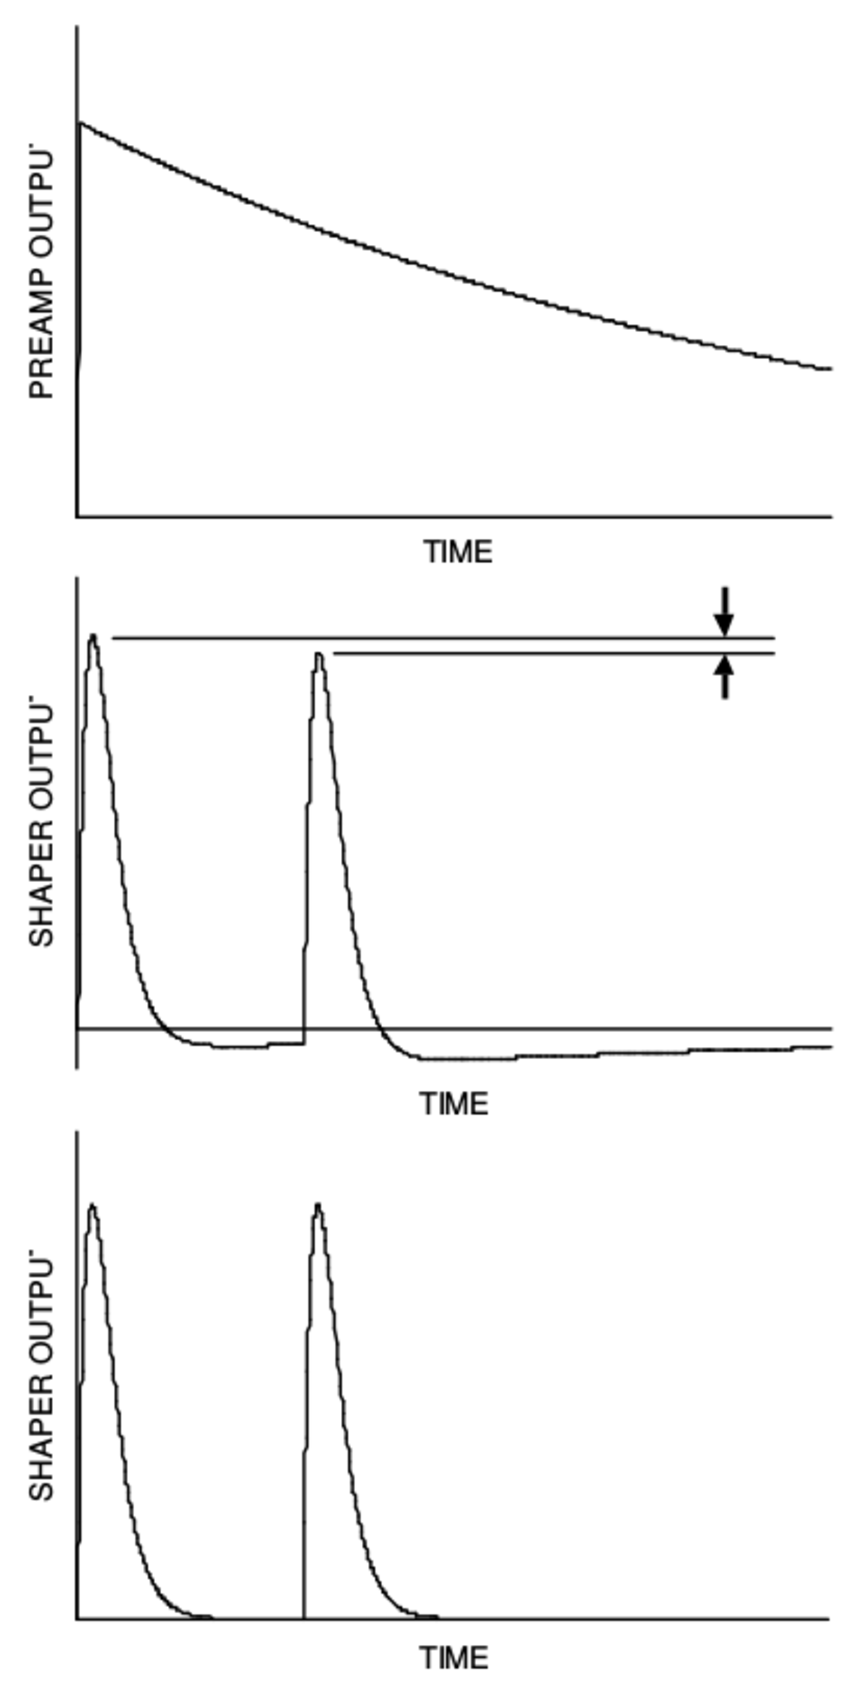
\includegraphics[width=0.7\textwidth]{d2/pz_graphs}
\end{center}
\end{column}
\end{columns}
\end{frame} 

\begin{frame}
\frametitle{Otros aspectos de la conformación de pulsos}
\framesubtitle{Compensación polo-cero}
\begin{columns}
\begin{column}{0.6\textwidth}
El ``cero'' cancela al ``polo'' del preamp cuando $R_{pz}C_d = R_FC_F$ 

\begin{itemize}
\item Técnica también utilizada para compensar las ``colas'' (tails) de los 
pulsos del detector:

``tail cancellation''
\item Crítico para el funcionamiento correcto del restaurador de linea de base
\end{itemize}
\begin{center}
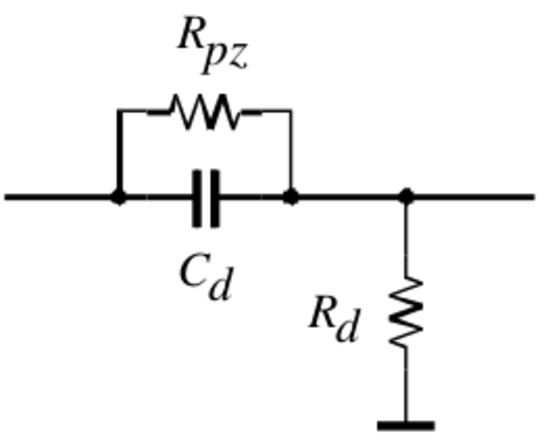
\includegraphics[width=0.4\textwidth]{d2/rpz_added}
\end{center}
\end{column}
\begin{column}{0.4\textwidth}
\begin{center}
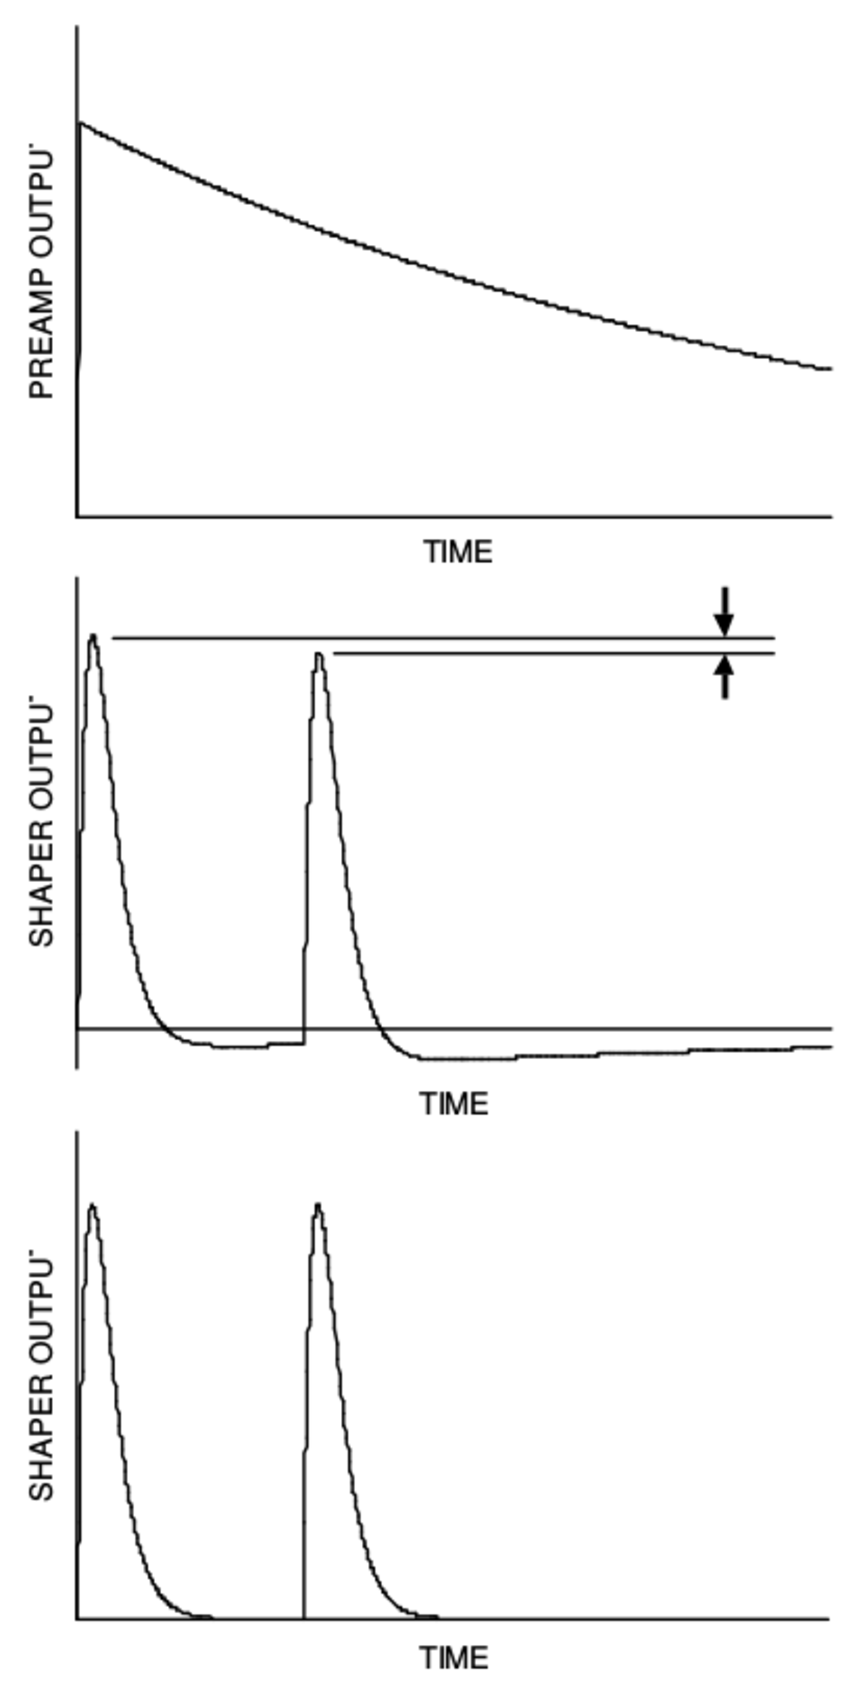
\includegraphics[width=0.7\textwidth]{d2/pz_graphs}
\end{center}
\end{column}
\end{columns}
\end{frame} 

\begin{frame}
\frametitle{Otros aspectos de la conformación de pulsos}
\framesubtitle{Conformación unipolar o bipolar} 
\begin{alertblock}{}
Pulso unipolar + $2^{do}$ diferenciador $\rightarrow$ pulso bipolar
\end{alertblock}
\begin{center}
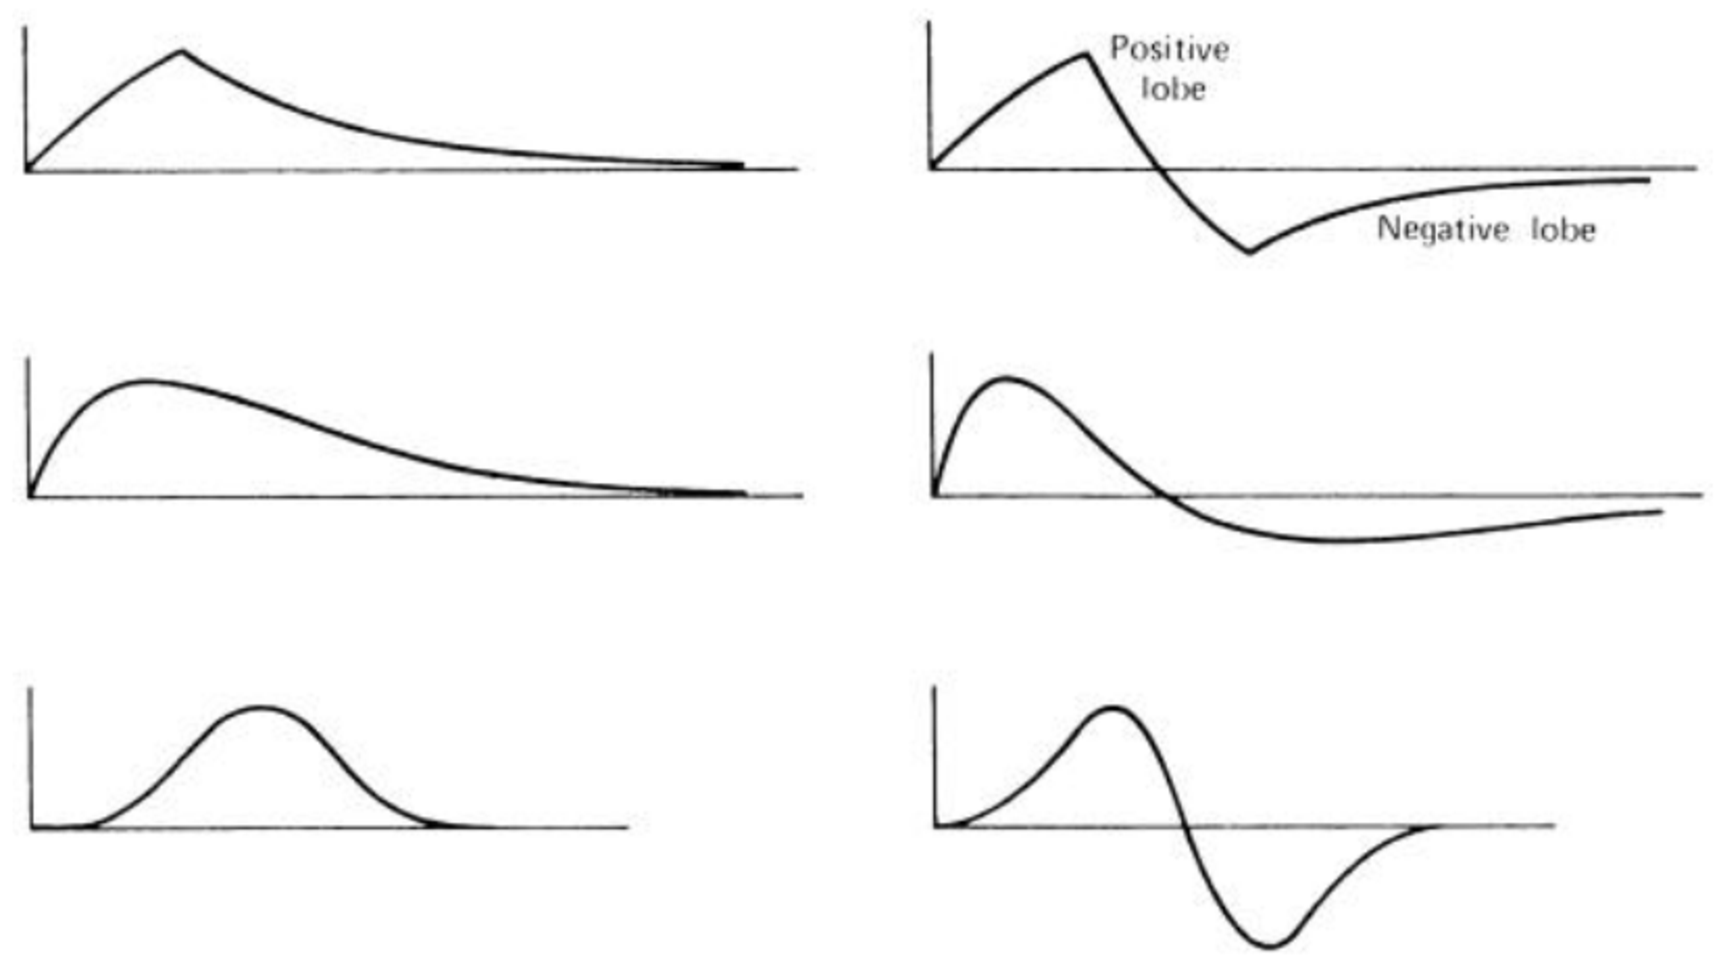
\includegraphics[width=0.65\textwidth]{d2/bipolar_unipolar_pulses}
\end{center}
Resolución electrónica con conformado bipolar típ. $25 - 50\,\%$ peor que con
el correpondiente conformado unipolar.
\end{frame} 

\begin{frame}
\frametitle{Otros aspectos de la conformación de pulsos}
\framesubtitle{Conformación unipolar o bipolar} 
Peeeeero...
\begin{itemize}
	\item El conformado bipolar elimina el cambio de la linea de base (ya que la 
componente DC es cero) 
	\item Ajuste para polo-cero menos crítico
	\item Agrega supresión de ruido de baja frecuencia
	\item No todas las mediciones requieren performance de ruido óptimo.

El conformado bipolar es más conveniente para el usuario (importante en sistemas 
grandes!). Es a menudo el método elegido
\end{itemize}
\end{frame} 

\begin{frame}
\frametitle{Otros aspectos de la conformación de pulsos}
\framesubtitle{Acumulamiento de pulsos (pulse pile-up) y rechazo de acumulamiento} 
\begin{alertblock}{}
Acumulamiento $\implies$ mediciones de amplitudes falsas
\end{alertblock}
\begin{columns}
\begin{column}{0.50\textwidth}

\alert{Caso 1:}

\begin{center}
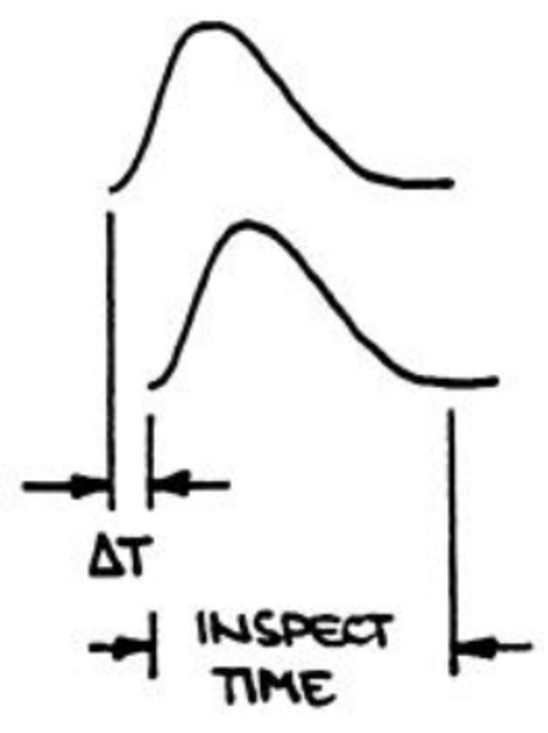
\includegraphics[width=0.6\textwidth]{d2/pileup_case1}
\end{center}

\end{column} 
\begin{column}{0.50\textwidth}
$$\Delta T < t_p$$

Ambas amplitudes de pico son afectadas por superposición 

$\implies$ rechazo de los dos pulsos

Tiempo muerto: $\Delta T$ + tiempo de inspección ($\sim$ ancho del pulso)
\end{column}
\end{columns}
\end{frame} 

\begin{frame}
\frametitle{Otros aspectos de la conformación de pulsos}
\framesubtitle{Acumulamiento de pulsos (pulse pile-up) y rechazo de acumulamiento} 
\begin{alertblock}{}
Acumulamiento $\implies$ mediciones de amplitudes falsas
\end{alertblock}
\begin{columns}
\begin{column}{0.40\textwidth}

\alert{Caso 2:}

\begin{center}
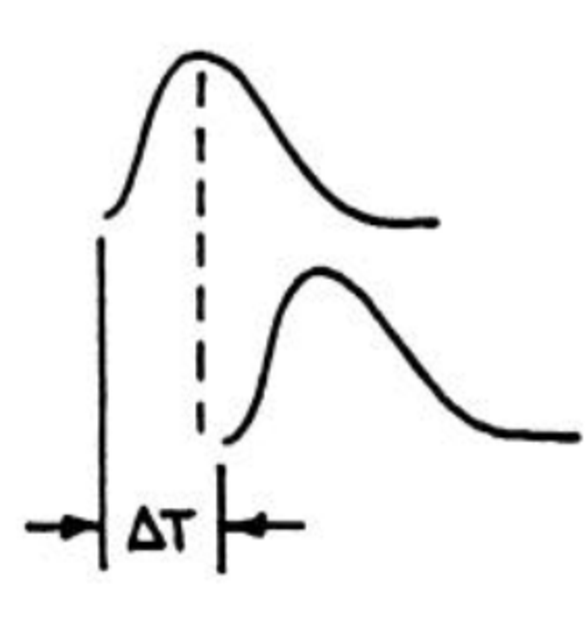
\includegraphics[width=0.75\textwidth]{d2/pileup_case2}
\end{center}

\end{column} 
\begin{column}{0.60\textwidth}
$\Delta T > t_p$ y \\
$\Delta T <$ tiempo de inspección, es decir tiempo donde la amplitud 
del primer pulso $<<$ resoulción

Amplitud de pico del primer pulso no afectado 

$\implies$ rechazo del $2^{do}$ pulso solamente

No hay tiempo muerto adicional si el $1^{er}$ pulso fue aceptado para 
digitalizar y el tiempo muerto del ADC $>$ ($\Delta T$ + tiempo de 
inspección)
\end{column}
\end{columns}
\end{frame} 

\begin{frame}
\frametitle{Otros aspectos de la conformación de pulsos}
\framesubtitle{Acumulamiento de pulsos (pulse pile-up) y rechazo de acumulamiento} 
\begin{center}
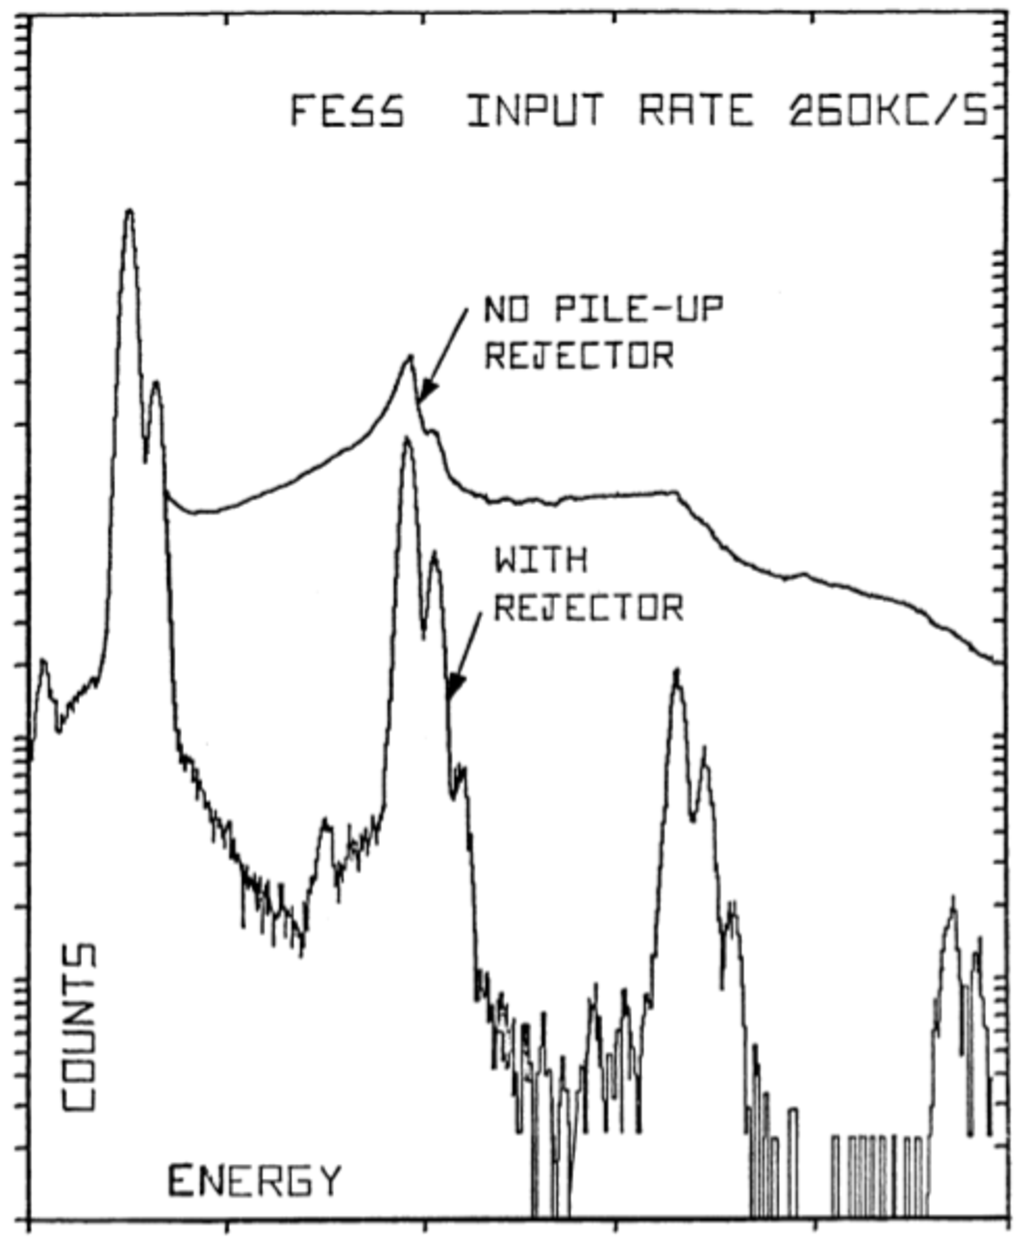
\includegraphics[width=0.48\textwidth]{d2/pileup_rejector_graph}
\end{center}
\end{frame} 

%\begin{frame}
%\frametitle{Definiciones (Cont.)}
%\begin{columns}
%\begin{column}{0.50\textwidth}
%\begin{block}{Electrónica dedicada para Auger}
%\begin{itemize}
%\item Poco flexible 
%\item Información limitada
%\item Número limitado de UBs (\alert{Unified Boards})
%\item Comunicación de datos por puerto serie
%\item	Tiempos de adquisición largos
%\item	Poco volumen de almacenamiento
%\item Sin control línea de base	
%\end{itemize}
%	\end{block}
%\end{column} 
%\begin{column}{0.50\textwidth}
%\fbox{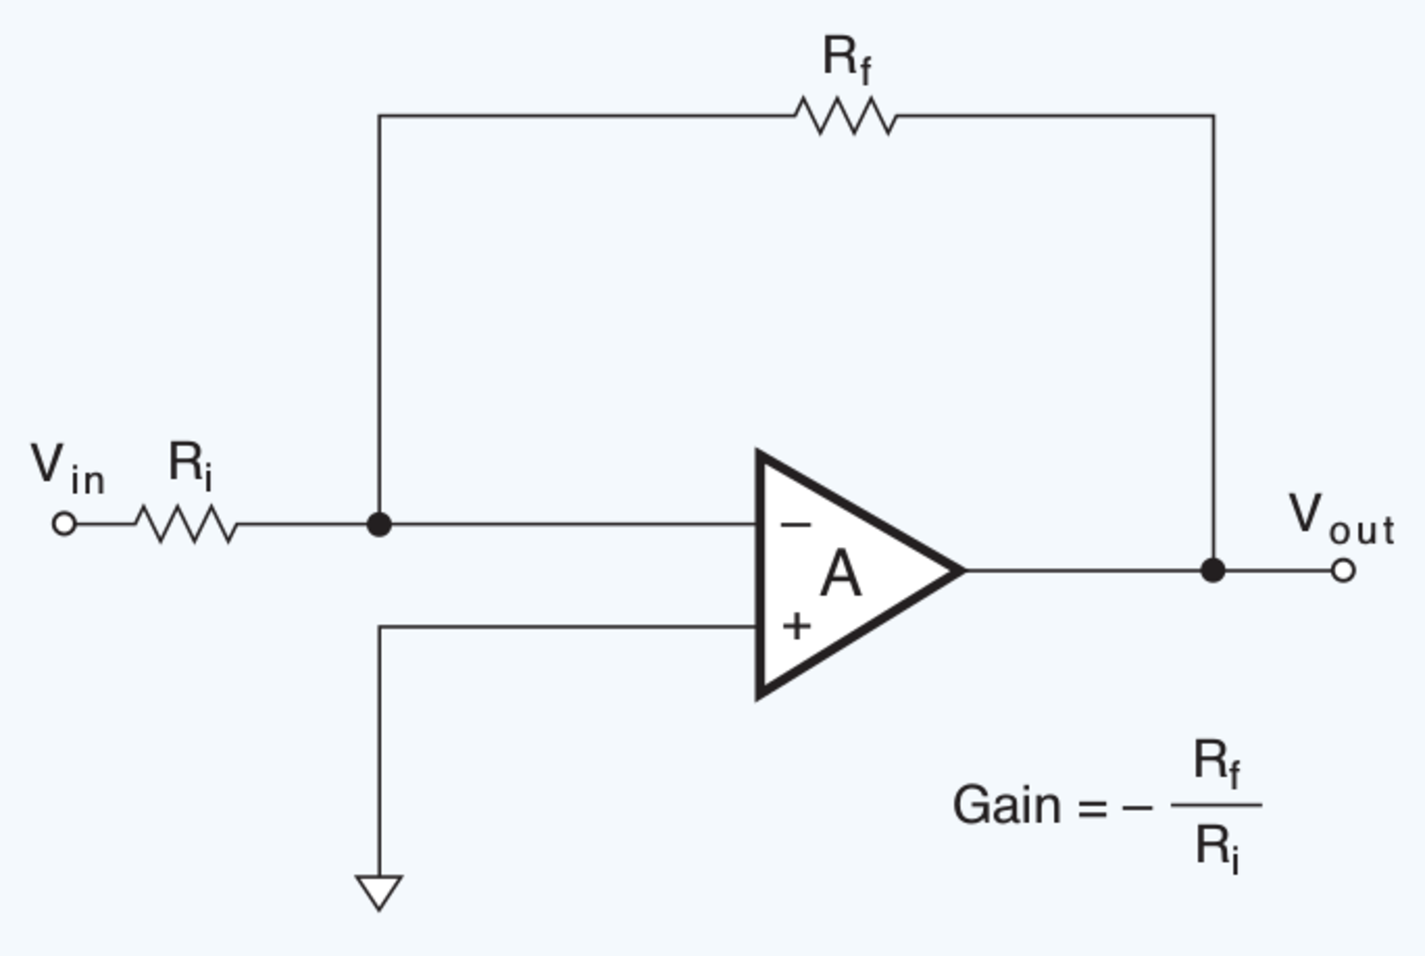
\includegraphics[width=\textwidth]{d2/ao_inversor}}
%		 \end{column}
%		\end{columns}
%\end{frame} 
%
%\begin{frame}
%	\frametitle{Definiciones (Cont.)}
%		\begin{columns}
%			\begin{column}{0.50\textwidth}
%				\begin{block}{Electrónica dedicada para Auger}
%		    	\begin{itemize}
%		      	\item Poco flexible 
%		      	\item Información limitada
%		      	\item Número limitado de UBs (\alert{Unified Boards})
%						\item Comunicación de datos por puerto serie
%						\item	Tiempos de adquisición largos
%						\item	Poco volumen de almacenamiento
%						\item Sin control línea de base	
%		    	\end{itemize}
%				\end{block}
%			\end{column} 
%		 	\begin{column}{0.50\textwidth}
%		  	\fbox{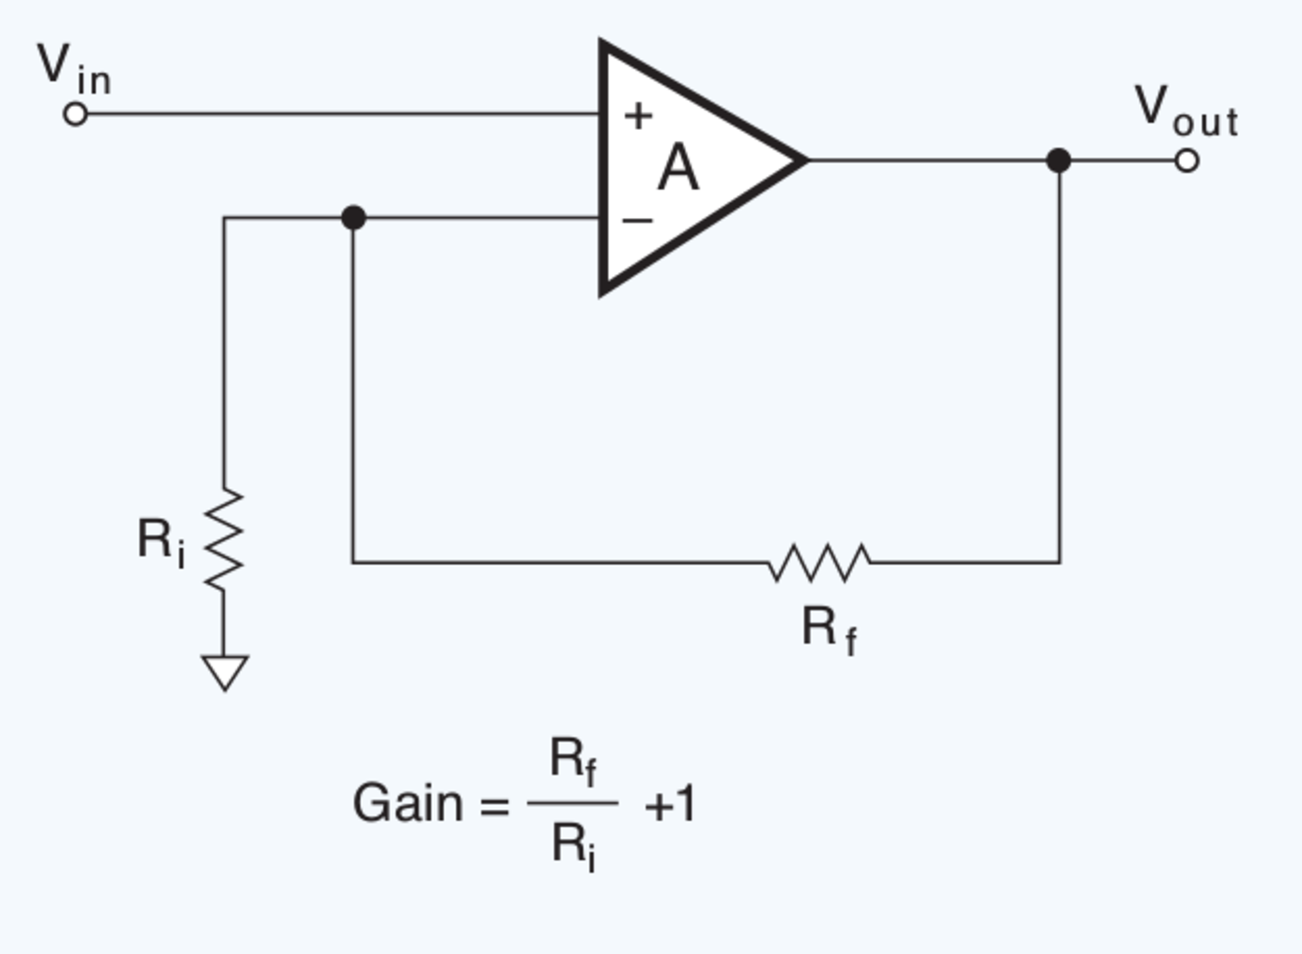
\includegraphics[width=\textwidth]{d2/ao_no_inversor}}
%		 \end{column}
%		\end{columns}
%\end{frame} 
%
%\begin{frame}
%	\frametitle{Definiciones (Cont.)}
%		\begin{columns}
%			\begin{column}{0.50\textwidth}
%				\begin{block}{Electrónica dedicada para Auger}
%		    	\begin{itemize}
%		      	\item Poco flexible 
%		      	\item Información limitada
%		      	\item Número limitado de UBs (\alert{Unified Boards})
%						\item Comunicación de datos por puerto serie
%						\item	Tiempos de adquisición largos
%						\item	Poco volumen de almacenamiento
%						\item Sin control línea de base	
%		    	\end{itemize}
%				\end{block}
%			\end{column} 
%		 	\begin{column}{0.50\textwidth}
%		  	\fbox{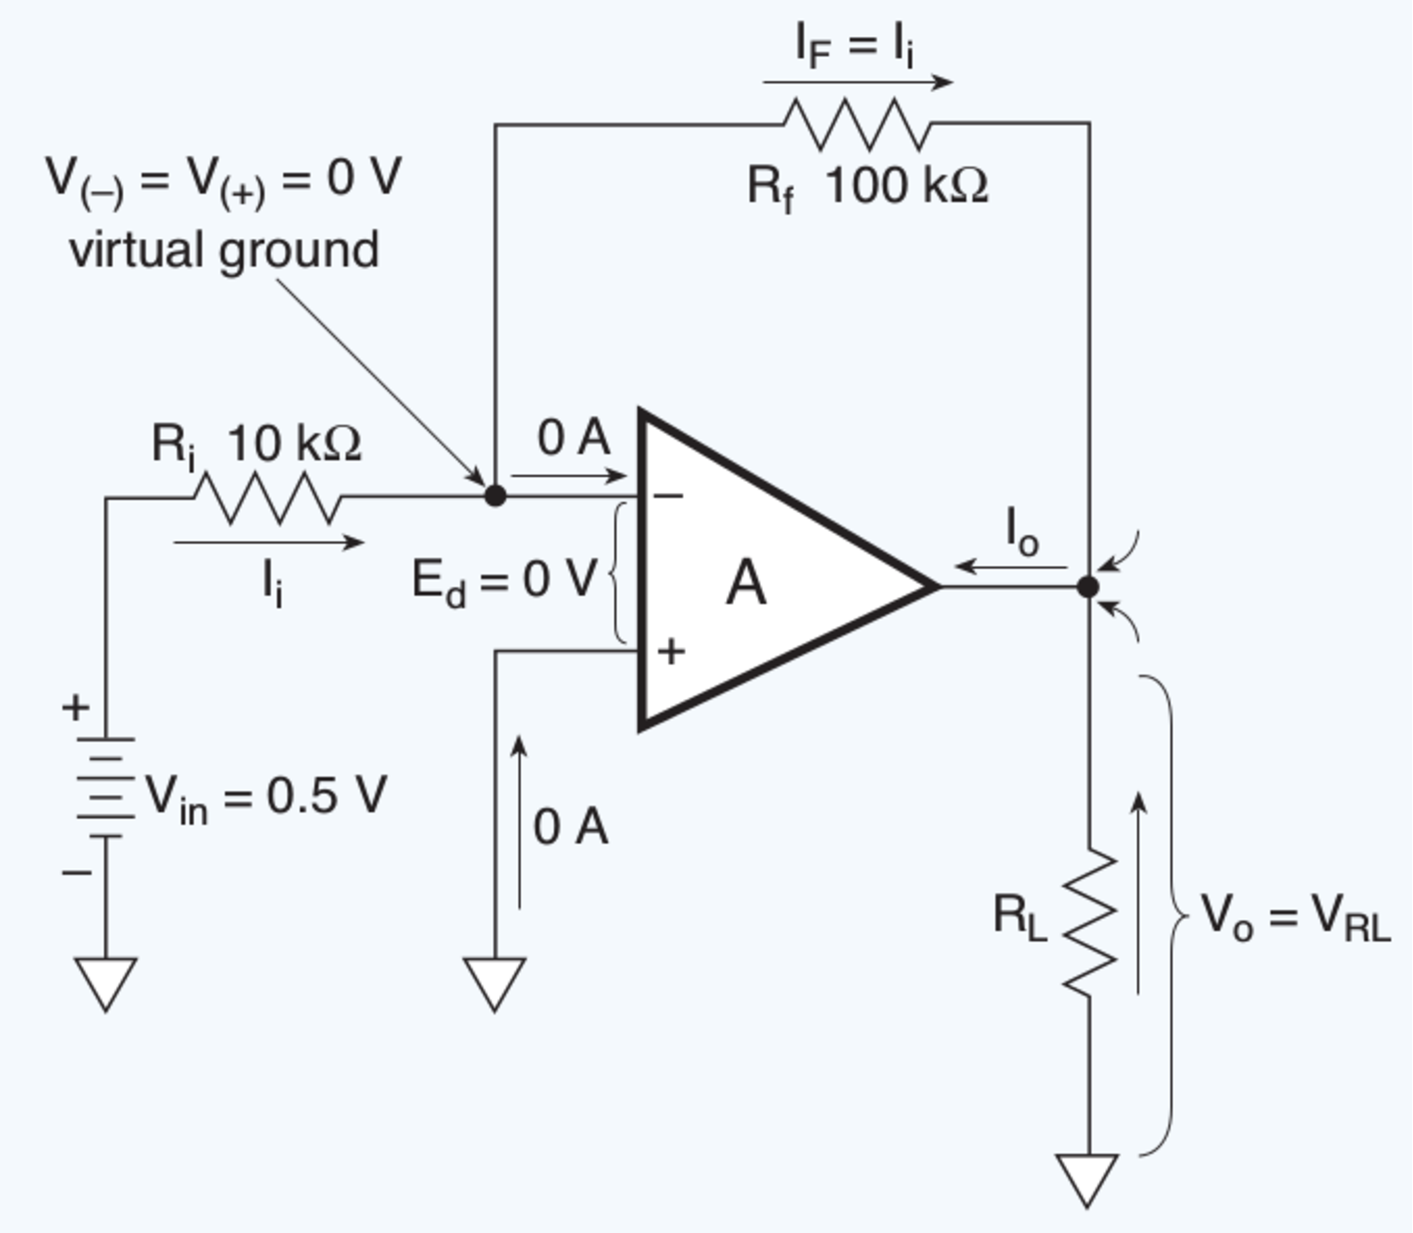
\includegraphics[width=\textwidth]{d2/inverting_stage}}
%		 \end{column}
%		\end{columns}
%\end{frame} 
%
%\begin{frame}
%	\frametitle{Definiciones (Cont.)}
%		\begin{columns}
%			\begin{column}{0.50\textwidth}
%				\begin{block}{Electrónica dedicada para Auger}
%		    	\begin{itemize}
%		      	\item Poco flexible 
%		      	\item Información limitada
%		      	\item Número limitado de UBs (\alert{Unified Boards})
%						\item Comunicación de datos por puerto serie
%						\item	Tiempos de adquisición largos
%						\item	Poco volumen de almacenamiento
%						\item Sin control línea de base	
%		    	\end{itemize}
%				\end{block}
%			\end{column} 
%		 	\begin{column}{0.50\textwidth}
%		  	\fbox{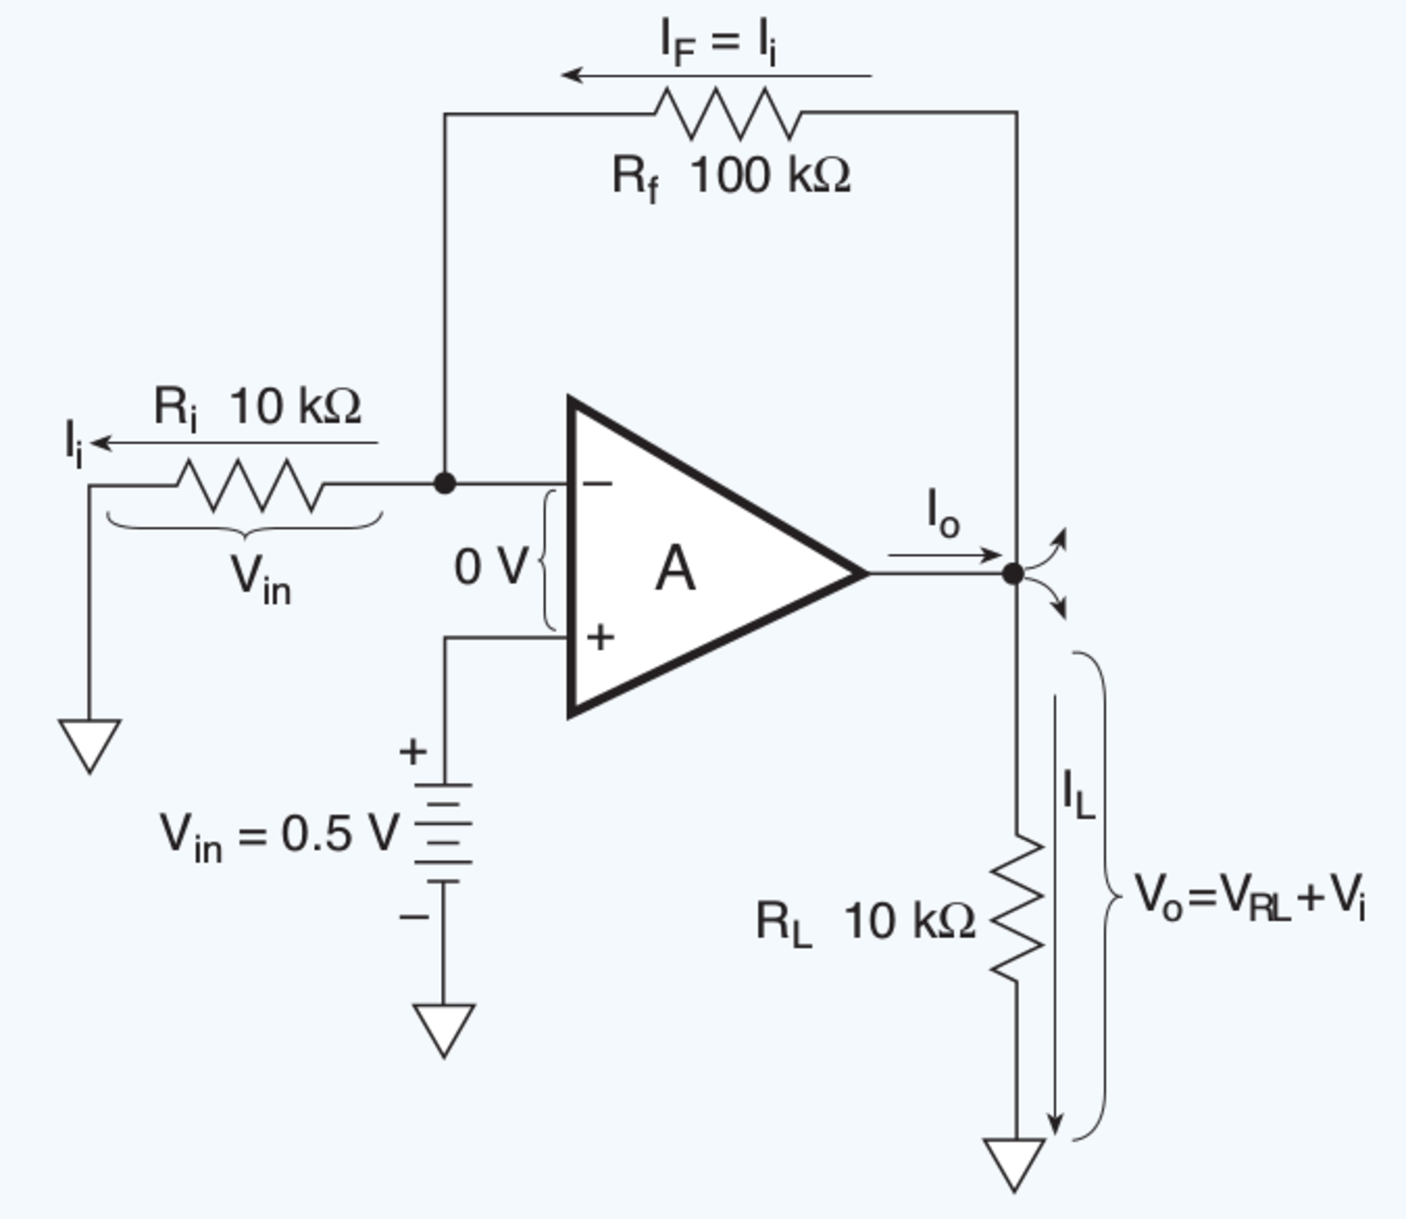
\includegraphics[width=\textwidth]{d2/noninverting_stage}}
%		 \end{column}
%		\end{columns}
%\end{frame} 
%
%\begin{frame}
%	\frametitle{Definiciones (Cont.)}
%		\begin{columns}
%			\begin{column}{0.50\textwidth}
%				\begin{block}{Electrónica dedicada para Auger}
%		    	\begin{itemize}
%		      	\item Poco flexible 
%		      	\item Información limitada
%		      	\item Número limitado de UBs (\alert{Unified Boards})
%						\item Comunicación de datos por puerto serie
%						\item	Tiempos de adquisición largos
%						\item	Poco volumen de almacenamiento
%						\item Sin control línea de base	
%		    	\end{itemize}
%				\end{block}
%			\end{column} 
%		 	\begin{column}{0.50\textwidth}
%		  	\fbox{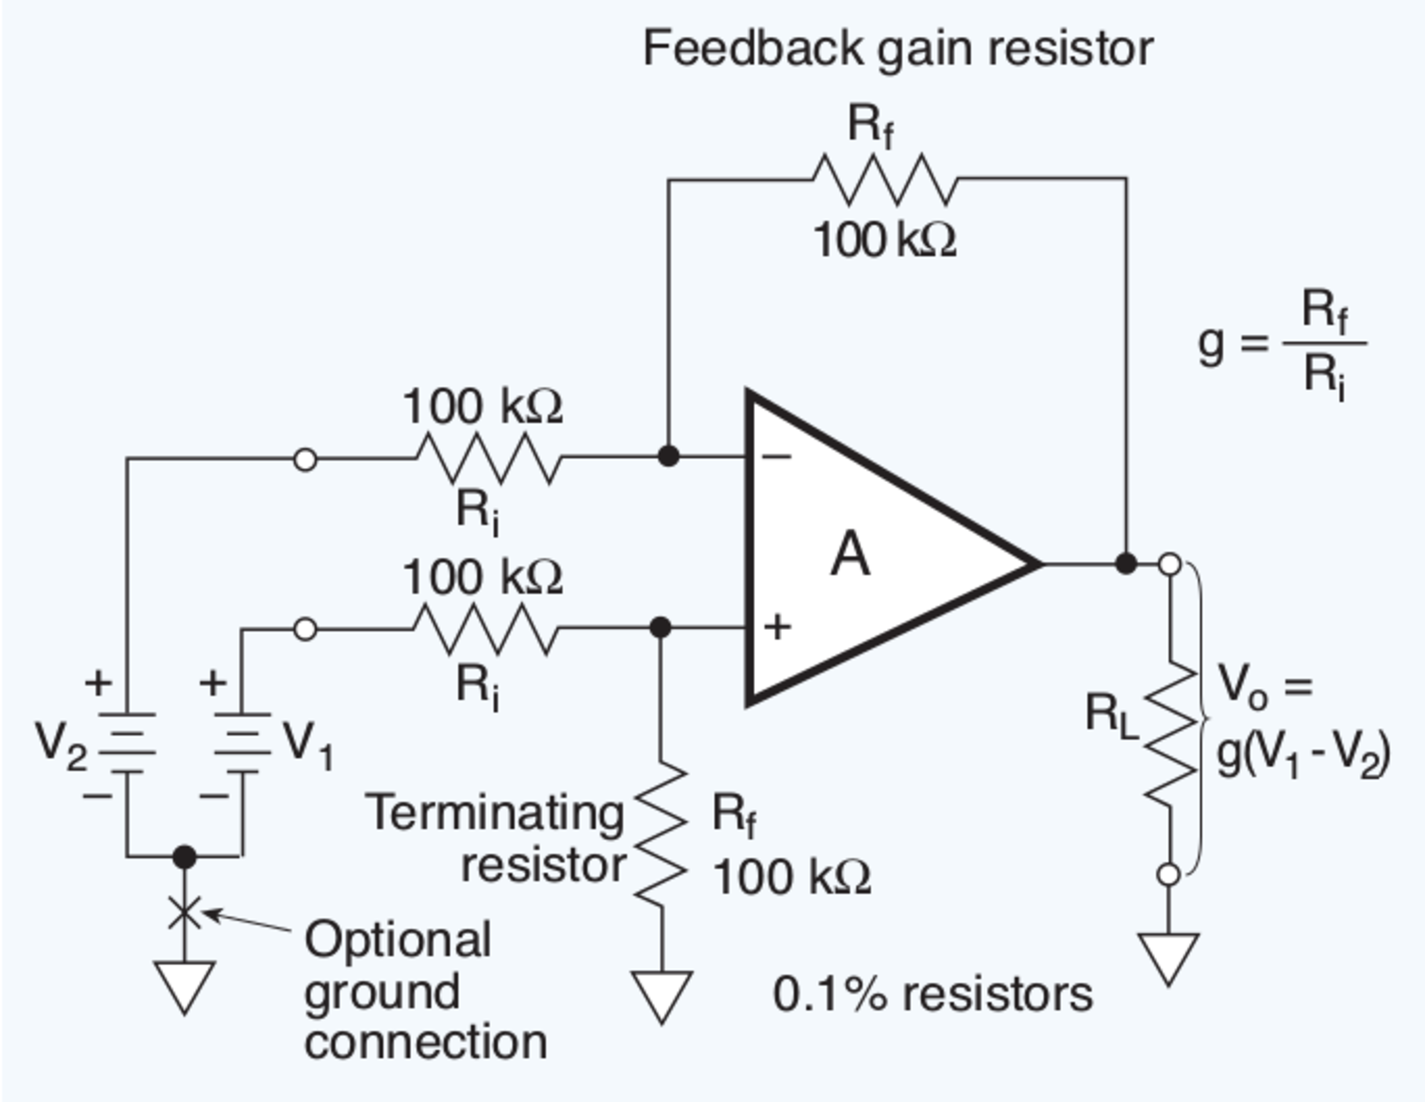
\includegraphics[width=\textwidth]{d2/differential_stage}}
%		 \end{column}
%		\end{columns}
%\end{frame} 
%
%\begin{frame}
%	\frametitle{Definiciones (Cont.)}
%		\begin{columns}
%			\begin{column}{0.50\textwidth}
%				\begin{block}{Electrónica dedicada para Auger}
%		    	\begin{itemize}
%		      	\item Poco flexible 
%		      	\item Información limitada
%		      	\item Número limitado de UBs (\alert{Unified Boards})
%						\item Comunicación de datos por puerto serie
%						\item	Tiempos de adquisición largos
%						\item	Poco volumen de almacenamiento
%						\item Sin control línea de base	
%		    	\end{itemize}
%				\end{block}
%			\end{column} 
%		 	\begin{column}{0.50\textwidth}
%		  	\fbox{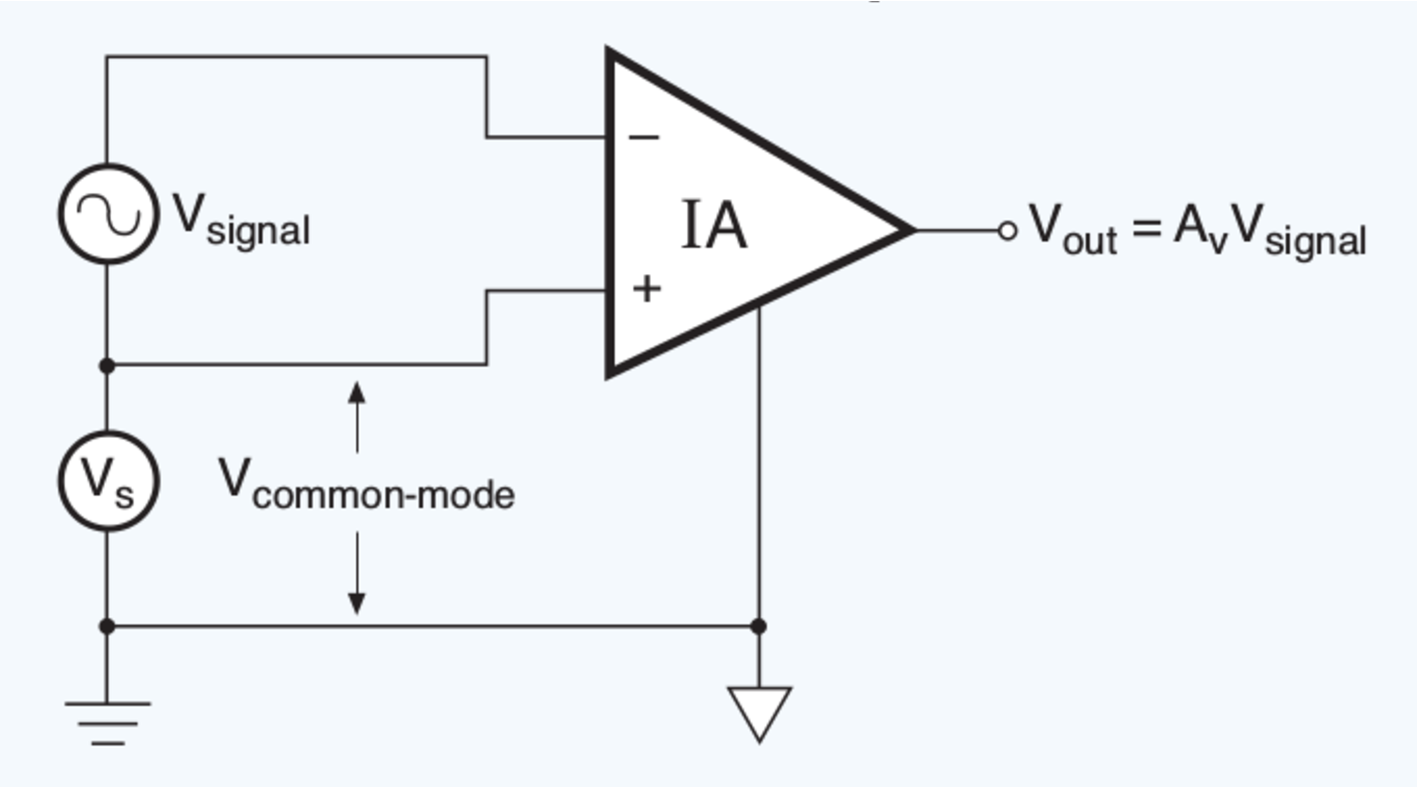
\includegraphics[width=\textwidth]{d2/instrumentation_amp_base}}
%		 \end{column}
%		\end{columns}
%\end{frame} 
%
%\begin{frame}
%	\frametitle{Definiciones (Cont.)}
%		\begin{columns}
%			\begin{column}{0.50\textwidth}
%				\begin{block}{Electrónica dedicada para Auger}
%		    	\begin{itemize}
%		      	\item Poco flexible 
%		      	\item Información limitada
%		      	\item Número limitado de UBs (\alert{Unified Boards})
%						\item Comunicación de datos por puerto serie
%						\item	Tiempos de adquisición largos
%						\item	Poco volumen de almacenamiento
%						\item Sin control línea de base	
%		    	\end{itemize}
%				\end{block}
%			\end{column} 
%		 	\begin{column}{0.50\textwidth}
%		  	\fbox{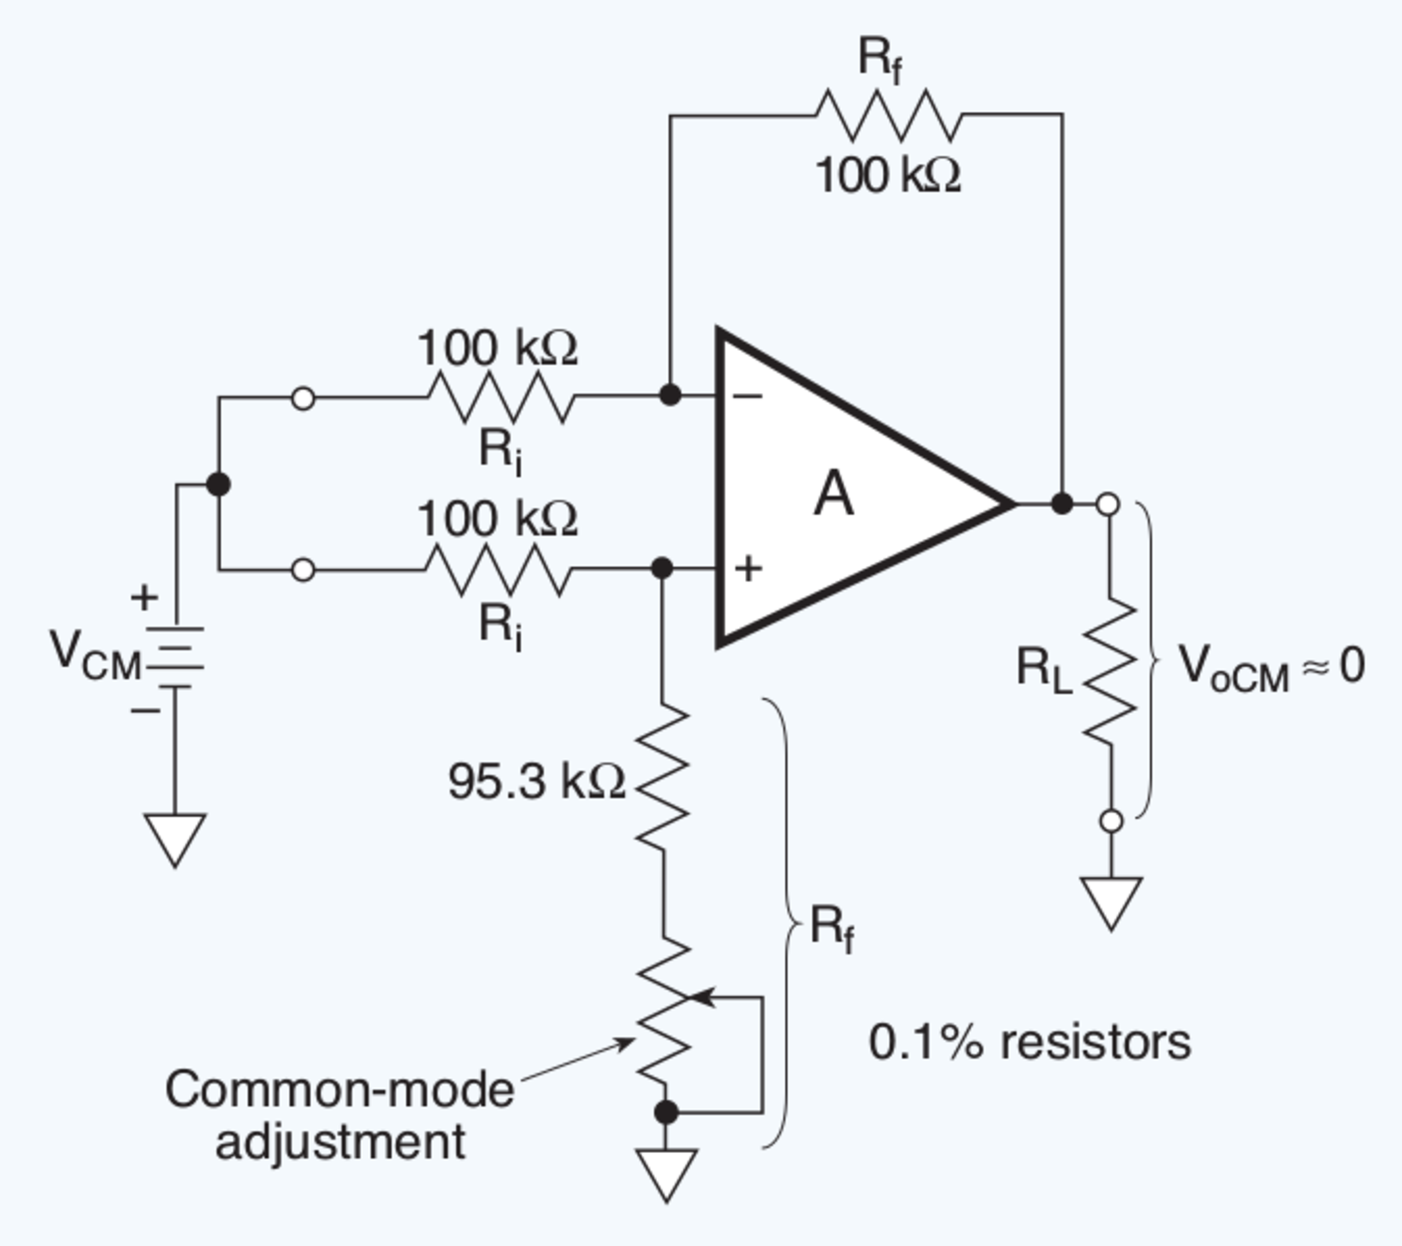
\includegraphics[width=\textwidth]{d2/CMRR_meas}}
%		 \end{column}
%		\end{columns}
%\end{frame} 
%
%\begin{frame}
%	\frametitle{Definiciones (Cont.)}
%		\begin{columns}
%			\begin{column}{0.50\textwidth}
%				\begin{block}{Electrónica dedicada para Auger}
%		    	\begin{itemize}
%		      	\item Poco flexible 
%		      	\item Información limitada
%		      	\item Número limitado de UBs (\alert{Unified Boards})
%						\item Comunicación de datos por puerto serie
%						\item	Tiempos de adquisición largos
%						\item	Poco volumen de almacenamiento
%						\item Sin control línea de base	
%		    	\end{itemize}
%				\end{block}
%			\end{column} 
%		 	\begin{column}{0.50\textwidth}
%		  	\fbox{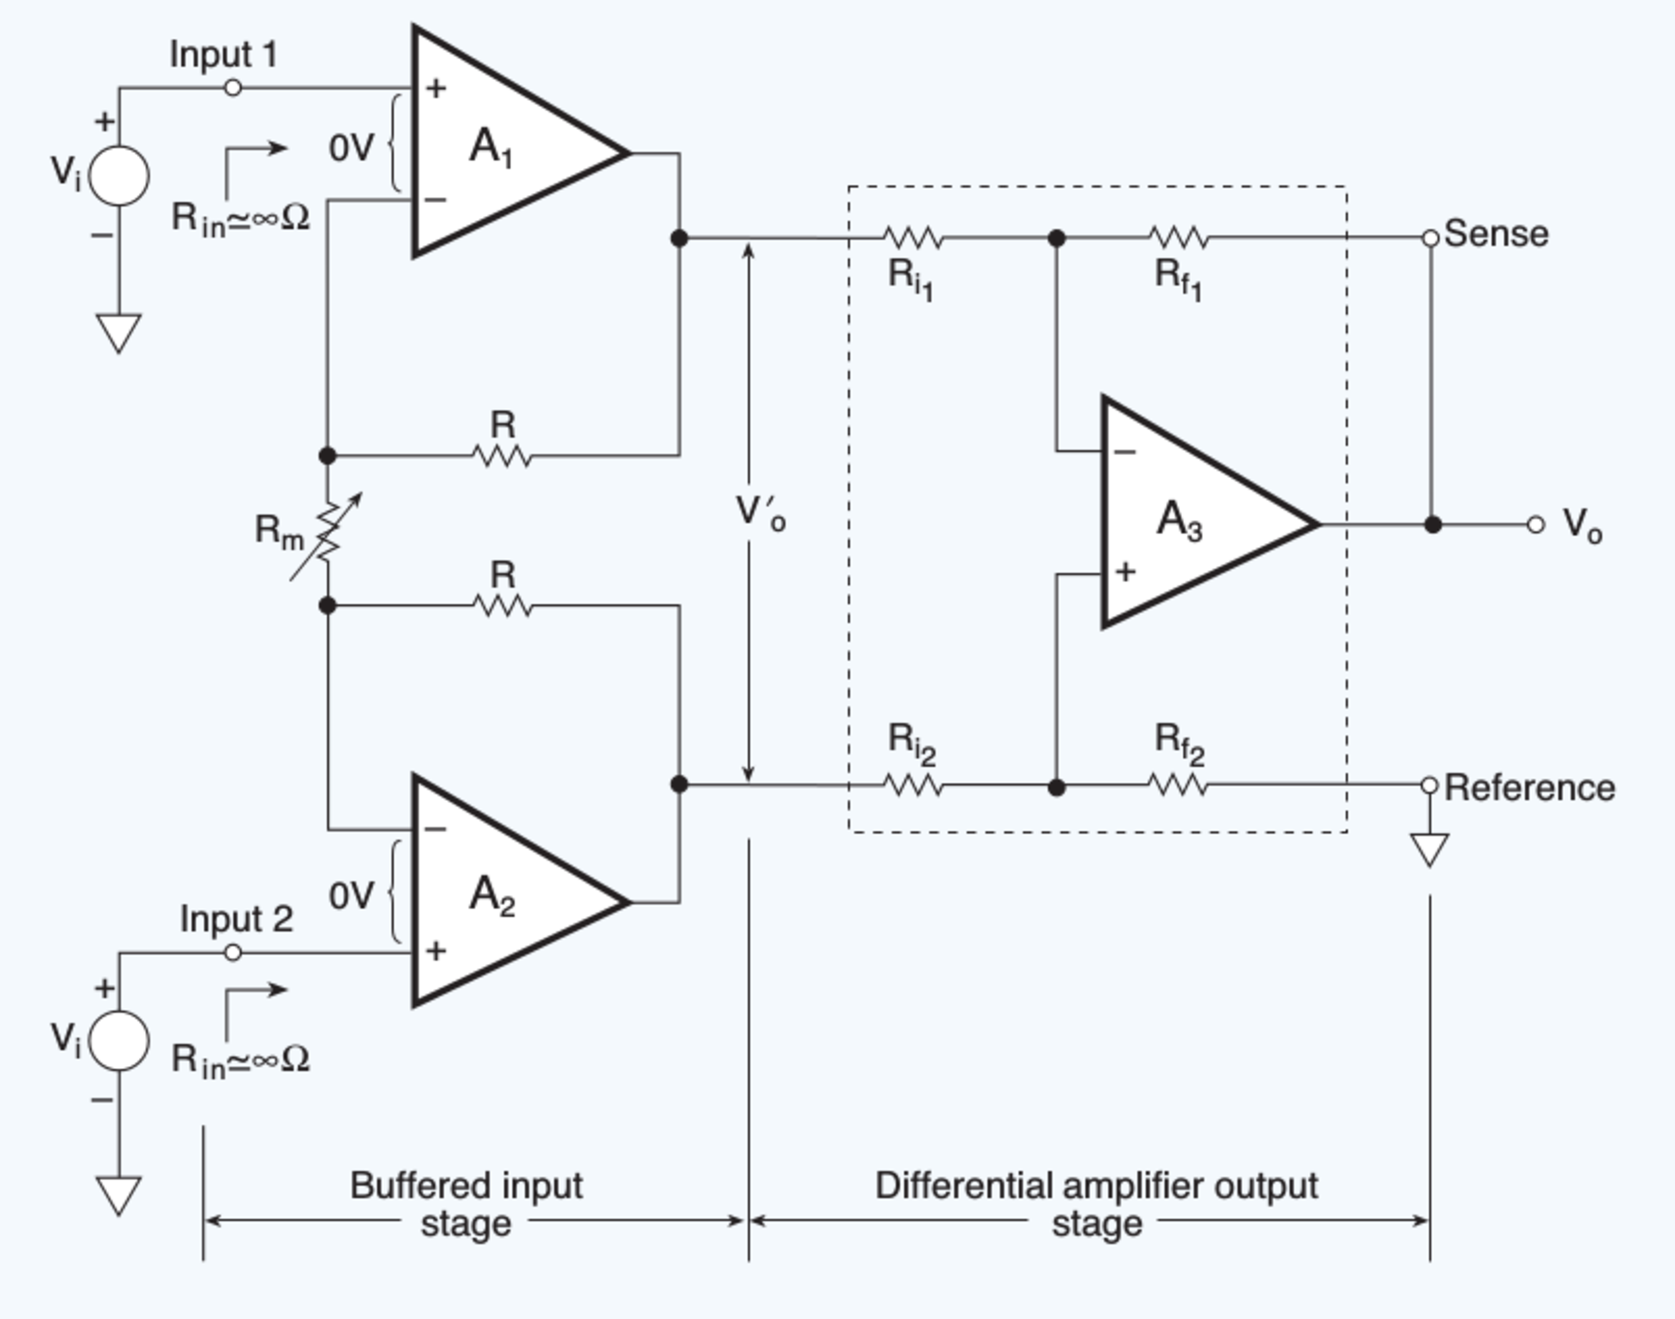
\includegraphics[width=\textwidth]{d2/instrumentation_amp}}
%		 \end{column}
%		\end{columns}
%\end{frame} 

%\begin{frame}
%\frametitle{Actualidad: ¿con qué contamos?}
%\begin{columns}
%\begin{column}{0.40\textwidth}
%\begin{block}{}
%\begin{itemize}[<+->]
%\item Placas de digitalización de 3 y 4 canales
%\item GPS para sincronizar los datos de los 
%distintos sitios
%\item Barómetro y sensor de temperatura
%\item Placa Nexys2 (FPGA Spartan 3E)
%\end{itemize}
%\end{block}
%\end{column} 
%\begin{column}{0.55\textwidth}
%%\only<1-2>{\fbox{\includegraphics[width=\textwidth]{d2/hardware_nahuelito}}}
%%\only<3-4>{\fbox{\includegraphics[width=\textwidth]{d2/placa_mx_2}}}
%\end{column}
%\end{columns}
%\end{frame} 
%
%\begin{frame}
%	\frametitle{Dificultades actuales}
%	\begin{alertblock}{}
%		\begin{itemize}
%		\item Hasta la aparición del sistema \alert{ACQUA}, \alert{ANNA}, etc
%					(aprox. noviembre de 2015) teníamos (casi) cada sitio una versión
%					diferente del \alert{firmware} de la FPGA 
%		\item No todos los sitios pueden estar online con sus datos (por diversas
%					razones, a veces ajenas a la electrónica)
%		\item Existencia de dos tipos de electrónicas (con características muy
%					diferentes)
%		\item Problemas contínuos con las placas de adquisición (cortos, falsos
%					contactos, soldaduras frías, etc) debido a que se ensamblan en casa
%		\end{itemize}
%	\end{alertblock}
%\end{frame} 
%
%\begin{frame}
%	\frametitle{Dificultades actuales}
%	\begin{alertblock}{}
%		\begin{itemize}
%		\item Los GPS Oncore están dejando de funcionar en casi todos los sitios y
%					nosotros tenemos la electrónica dedicada a ese GPS particular (que ya no se
%					fabrica más, además)
%		\item Sensores de PyT (HP03) difíciles de conseguir hoy en día
%		\item Las placas Nexys2 \alert{¡dejaron de fabricarse!} y constituyen el
%					corazón de lo que tenemos actualmente
%		\item ...todo tiene un final, todo termina...
%		\end{itemize}
%	\end{alertblock}
%\end{frame} 

%\begin{frame}
%	\frametitle{Futuro: ¿cuál es la opción?}
%	\begin{columns}
%		\begin{column}{0.40\textwidth}
%			\begin{block}{}
%	    	\begin{itemize}[<+->]
%	      	\item RedPitaya: 2 canales @ 50\,MHz (adquisición)
%	      	\item Capacidad de conexión y envío de datos a puntos remotos
%	      	\item Se pueden conectar los sensores que necesitemos 
%					\item Mucha \alert{flexibilidad} (¡justo lo que queremos!)
%	    	\end{itemize}
%			\end{block}
%		\end{column} 
%	 	\begin{column}{0.55\textwidth}
%	  	%\fbox{\includegraphics[width=\textwidth]{d2/rp_freecad_up}}
%	 \end{column}
%	\end{columns}
%\end{frame} 
%
%\begin{frame}
%	\frametitle{Futuro: RedPitaya}
%		\begin{block}{}
%	  	\begin{itemize}
%	    	\item Esperamos tener el sistema listo para fin de año (2016) o mediados
%							del año que viene
%	    	\item Es poca la ganancia en ancho de banda, respecto a lo que ya
%							tenemos. Pero se gana mucho en flexibilidad.
%	    	\item Todavía hay que trabajar, tanto en hardware como en software
%				\item ... pero para eso estamos dentro de una comunidad... y el \alert{trabajo
%							colaborativo} debe afianzarse
%	  	\end{itemize}
%		\end{block}
%\end{frame} 

%------------------------------------------------------------------------------
%\section{Adaptación}
%%------------------------------------------------------------------------------
%
%\begin{frame}
%  \begin{center}
%    \Huge{\color{blue}{Adaptación: entrada y salida}}
%  \end{center}
%\end{frame}
%
%\subsection{El amplificador de instrumentación}
%
%\begin{frame}
%\frametitle{Las herramientas}
%  \begin{columns}
%    \begin{column}{0.45\textwidth}
%      \begin{block}{Nexys2}
%        \begin{itemize}
%          \item  Familia FPGA Spartan3E
%          \item  60 pines E/S disponibles para nuestro uso (144 en total)
%          \item  El firmware LAGO ocupa aprox. el 70\% de sus recursos internos
%                 (memoria, bloques de I/O, etc.)
%        \end{itemize}
%      \end{block}
%    \end{column} 
%    \begin{column}{0.65\textwidth}
%      \includegraphics[width=0.8\textwidth]{d2/instrumentation_amp}
%    \end{column}
%  \end{columns}
%\end{frame}
%
%\subsection{Impedancia de fuente y de entrada}
%
%\begin{frame}
%\frametitle{Impedancia de fuente y de entrada}
%\begin{columns}
%\begin{column}{0.50\textwidth}
%	\begin{block}{Electrónica dedicada para Auger}
%\begin{itemize}
%\item Poco flexible 
%\item Información limitada
%\item Número limitado de UBs (\alert{Unified Boards})
%\item Comunicación de datos por puerto serie
%\item	Tiempos de adquisición largos
%\item	Poco volumen de almacenamiento
%\item Sin control línea de base	
%\end{itemize}
%\end{block}
%\end{column} 
%\begin{column}{0.50\textwidth}
%\fbox{\includegraphics[width=\textwidth]{d2/tc_input}}
%\end{column}
%\end{columns}
%\end{frame} 
%
%\begin{frame}
%\frametitle{Definiciones (Cont.)}
%\begin{columns}
%\begin{column}{0.50\textwidth}
%\begin{block}{Electrónica dedicada para Auger}
%\begin{itemize}
%\item Poco flexible 
%\item Información limitada
%\item Número limitado de UBs (\alert{Unified Boards})
%\item Comunicación de datos por puerto serie
%\item Tiempos de adquisición largos
%\item Poco volumen de almacenamiento
%\item Sin control línea de base	
%\end{itemize}
%\end{block}
%\end{column} 
%\begin{column}{0.50\textwidth}
%\fbox{\includegraphics[width=\textwidth]{d2/z_input}}
%\end{column}
%\end{columns}
%\end{frame} 

%------------------------------------------------------------------------------
\section{Amplificación}
%------------------------------------------------------------------------------

\begin{frame}
  \begin{center}
    \Huge{\color{blue}{Amplificación de señales}}
  \end{center}
\end{frame}

\begin{frame}
\frametitle{Preamplificadores}
\begin{itemize}
\item La carga creada dentro de un detector es recogida por el preamp
\item Un preamp es el primer componente en una cadena de procesamiento de
señal de un detector de radiación
\item La naturaleza de la señal generada por el detector \alert{determina la
arquitectura de la entrada} del preamp
\item A pesar de su nombre, el preamp no actúa como amplificador (sólo
significa ``antes'', es decir, ``pre'' al amplificador), sino que actúa como una
interfaz entre el detector y la electrónica de procesamiento de pulsos que sigue 
\item La función principal de un preamp es extraer la señal del detector
{\color{blue}sin degradar significativamente la relación señal/ruido (SNR)
intrínseca}
\end{itemize}
\end{frame}

\begin{frame}
\frametitle{Preamplificadores}
\begin{itemize}
\item Requisitos importantes para el preamp son:
\begin{itemize}
\item Terminar la capacitancia rápidamente para maximizar la relación
señal-ruido. La longitud del cable entre el preamp y el detector se mantiene al
mínimo también debido a la misma razón
\item Tener una impedancia de salida baja: es decir, proporcionar una fuente de baja
impedancia para el amplificador
\item Debe proporcionar una carga de alta impedancia para el detector
\item Rango dinámico
\item Tiempo de respuesta
\item Consumo
\end{itemize}
\end{itemize}
\end{frame}

\begin{frame}
\frametitle{Preamplificador = Amplificador de entrada}
\begin{block}{}
\begin{itemize}
\item Generalmente ubicado en el detector
\item Amplifica la señal optimizando la relación señal-ruido (SNR)
\item Tres configuraciones básicas:
\begin{itemize}
\item Preamplificador de voltaje
\item Preamplificador de corriente
\item Preamplificador de carga
\end{itemize}
\end{itemize}
\end{block}
\end{frame}

\begin{frame}
\frametitle{Preamplificador de voltaje}
\begin{columns}
\begin{column}{0.4\textwidth}
\includegraphics[width=\textwidth]{d2/preamp_v}
\end{column}
\begin{column}{0.6\textwidth}
\begin{itemize}
\item Su impedancia de salida debe ser chica comparada con la de la
siguiente etapa 
\item \alert{La impedancia de entrada ($R_a$) es muy grande para que no drene corriente
del detector}
\item La ganancia $A$ depende de los componentes externos
\item Se usa el criterio $$t_d \ll R_aC_d$$ para determinar si el preamp
es adecuado para el detector ($t_d =$ tiempo de colección )
\end{itemize}
\end{column}
\end{columns}
\end{frame}

\begin{frame}
\frametitle{Preamplificador de voltaje}
\begin{block}{}
Para sensores que generan señales de tensión o como segunda etapa para sensores
que generan señales de corriente
\end{block}
\begin{columns}
\begin{column}{0.5\textwidth}
\includegraphics[width=\textwidth]{d2/voltage_preamplifier}
\end{column}
\begin{column}{0.5\textwidth}
$$V_{out} = \frac{Q_{in}}{C_{tot}}$$

$$C_{tot} = C_{det} + C_{conn} + C_{in\_pre}$$
\end{column}
\end{columns}
\begin{block}{}
\alert{$C_{tot}$} puede cambiar en función de los parámetros de trabajo del detector
$\rightarrow$ cambios en \alert{$V_{out}$}
\end{block}
\end{frame}

\begin{frame}
\frametitle{Preamplificador de corriente}
\begin{columns}
\begin{column}{0.4\textwidth}
\includegraphics[width=\textwidth]{d2/preamp_i}
\end{column}
\begin{column}{0.6\textwidth}
\begin{itemize}
\item Para aplicaciones en las que es necesario medir la corriente instantánea
circulando por el detector
\item \alert{La impedancia de entrada ($R_a$) debe mantenerse lo más baja posible,
comparada con la impedancia de salida del detector}
\item Para determinar si el preamp es adecuado para el detector se usa el
criterio $$t_d \gg R_sC_d$$ 

\end{itemize}
\end{column}
\end{columns}
\end{frame}

\begin{frame}
\frametitle{Preamplificador de corriente}
\begin{columns}
\begin{column}{0.5\textwidth}
\includegraphics[width=\textwidth]{d2/current_preamplifier_zin}
\end{column}
\begin{column}{0.5\textwidth}
\begin{center}
$V_{out} = -AV_{in}$

$V_{out} - V_{in} = -R_f i_{in}$

$V_{out} = -R_f i_{in}\left(\frac{1}{1+\frac{1}{A}}\right)$

\vspace{7mm}
$\therefore \alert{V_{out} \approx -R_f i_{in}}$
\end{center}
\end{column}
\end{columns}
\begin{block}{Impedancia de entrada}
$V_{out} = -AV_{in}$

$V_{out} - V_{in} = -R_f i_{in}$

$-R_f i_{in} \left(\frac{1}{1+\frac{1}{A}}\right) = -AV_{in} \rightarrow  V_{in}
= \frac{R_f i_{in}}{1 + A} \rightarrow \alert{Z_{in} =
\frac{R_f}{1 + A}}$
\end{block}
\end{frame}

\begin{frame}
\frametitle{Preamplificador de corriente}
\begin{block}{Contribución de $C_{in}$}
\begin{itemize}
\item La señal de entrada es convolucionada con una exponencial
\item Incrementando $R_f$ se incrementan tanto la sensibilidad del
preamplificador como el $\tau$
\end{itemize}
\end{block}
\begin{columns}
\begin{column}{0.5\textwidth}
\includegraphics[width=\textwidth]{d2/current_preamplifier_cin_contribution}
\end{column}
\begin{column}{0.5\textwidth}\centering
$Z_{in} = \frac{R}{1 + j\omega R C}$
\end{column}
\end{columns}
\end{frame}

\begin{frame}
\frametitle{Preamplificador de carga}
\begin{columns}
\begin{column}{0.4\textwidth}
\includegraphics[width=\textwidth]{d2/preamp_q}
\end{column}
\begin{column}{0.6\textwidth}
\begin{itemize}
\item La carga acumulada en la capacitancia del detector es integrada en otro
capacitor
\item El potencial sobre este último capacitor es proporcional a la carga
original del detector 
\item \alert{La impedancia del preamp ($R_a$) debe ser grande para que toda la
carga se integre en $C_f$ ($Q_f \approx Q_d$)}
\end{itemize}
\end{column}
\end{columns}
\end{frame}

\begin{frame}
\frametitle{Preamplificador de carga}
\begin{columns}
\begin{column}{0.5\textwidth}
\includegraphics[width=\textwidth]{d2/charge_preamplifier_zin}
\end{column}
\begin{column}{0.5\textwidth}
\begin{center}
$V_{out} = -AV_{in}$

\vspace{2mm}
$V_{out} - V_{in} = -\frac{i_{in}(\omega)}{j \omega C_f}$

\vspace{2mm}
$V_{out} = -\frac{i_{in}(\omega)}{j \omega C_f}\left(\frac{1}{1+\frac{1}{A}}\right)$

\vspace{2mm}
$\therefore \alert{V_{out} \approx -\frac{i_{in}(\omega)}{j \omega C_f}}$

\vspace{1.5mm}
$i_{in}(t) = Q_{in}\delta (t) \qquad V_{out}(t) = -\frac{Q(t)}{C_f}$
\end{center}
\end{column}
\end{columns}
\begin{block}{Impedancia de entrada}
$V_{out} = -AV_{in} \qquad V_{out} = -\frac{i_{in}(\omega)}{j \omega
C_f}\left(\frac{1}{1+\frac{1}{A}}\right)$

\vspace{1.5mm}
$-\frac{i_{in}(\omega)}{j \omega C_f}\left(\frac{1}{1+\frac{1}{A}}\right) =
-AV_{in} \alert{\rightarrow} V_{in} = \frac{i_{in}(\omega)}{j \omega C_f (1 + A)}$

\vspace{1.5mm}
\alert{$C_{in} = (1 + A) C_f$}
\end{block}
\end{frame}

\begin{frame}
\frametitle{Preamplificador de carga}
\begin{block}{¿Cuánta señal se pierde?}
\begin{columns}
\begin{column}{0.5\textwidth}
\includegraphics[width=\textwidth]{d2/charge_preamplifier_signal_loose}
\end{column}
\begin{column}{0.5\textwidth}
\begin{center}
$\frac{Q_{amp}}{(1 + A) C_f} = \frac{Q}{(1 + A)C_f + C_t}$

\vspace{2mm}
\alert{$Q_{amp} = \frac{Q}{1 + \frac{C_t}{(1 + A)C_f}}$}
\end{center}
\end{column}
\end{columns}
\end{block}
\begin{block}{Ejemplo}
$A = 10^3$; $C_f = 1\,pF$

\vspace{2mm}
$C_t = 10\,pF \rightarrow \frac{Q_{ampl}}{Q} = 0.99$

\vspace{2mm}
$C_t = 100\,pF \rightarrow \frac{Q_{ampl}}{Q} = 0.90$
\end{block}
\end{frame}

\begin{frame}
\begin{center}
  {\color{red}\Huge{¿Cuál amplificador elegir?}}
\end{center}
\end{frame}

\begin{frame}
\frametitle{¿Amplificador de voltaje, corriente o carga?}
\begin{block}{}
\begin{itemize}
\item En los amplificadores de voltaje $R_s$ aumenta el voltaje, pero también el
voltaje de ruido de entrada
\item El amplificador de corriente (o transimpedancia) permite superar las
limitaciones del amplificador de voltaje en términos de ganancia por ancho de
banda, aunque a costa de mayor inestabilidad.
\end{itemize}
\end{block}
\end{frame}

%\begin{frame}
%  \fbox{\includegraphics[width=0.6\textwidth]{d2/TIA_general}}
%\end{frame}
%
%\begin{frame}
%  \fbox{\includegraphics[width=0.6\textwidth]{d2/TIA_no_inversor}}
%\end{frame}
%
%\begin{frame}
%  \fbox{\includegraphics[width=0.6\textwidth]{d2/CFA_ideal}}
%\end{frame}
%
%\begin{frame}
%  \fbox{\includegraphics[width=0.6\textwidth]{d2/esquema_det_TIA}}
%\end{frame}
%
%------------------------------------------------------------------------------
\section{Ruido en los amplificadores} %esta parte sacar de Spieler /home/arnaldi/biblioteca/electronica/spieler/
%------------------------------------------------------------------------------

\begin{frame}
\frametitle{Ruido en amplificadores}
Consideremos una cadena de dos amplificadores (o dispositivos amplificadores), 
con ganancias $A_1$ y $A_2$, y niveles de ruido de entrada $N_1$ y $N_2$.

Se aplica una señal $S$ al primer amplificador, de modo que la relación 
señal/ruido de entrada es $S/N_1$
\begin{center}
\includegraphics[width=.7\textwidth]{d2/two_amp_snr}
\end{center}
A la salida del primer amplificador la señal es $A_1 S$ y el ruido $A_1 N$.
%
%Ambos son amplificados por el segundo amplificador, pero además el segundo 
%amplificador contribuye su ruido, por lo que la relación señal-ruido en la 
%salida del segundo amplificador es
%
%$$\left(\frac{S}{N}\right)^2 = \frac{(S A_1 A_2)^2}{(N_1 A_1 A_2)^2 + (N_2 A_2)^2} = \frac{S^2}{N_1^2 + \left(\frac{N_2}{A_1}\right)^2}$$
\end{frame}

\begin{frame}
\frametitle{Ruido en amplificadores}
%Consideremos una cadena de dos amplificadores (o dispositivos amplificadores), 
%con ganancias $A_1$ y $A_2$, y niveles de ruido de entrada $N_1$ y $N_2$.
%
%Se aplica una señal $S$ al primer amplificador, de modo que la relación 
%señal/ruido de entrada es $S/N_1$
%\begin{center}
%\includegraphics[width=.7\textwidth]{d2/two_amp_snr}
%\end{center}
%A la salida del primer amplificador la señal es $A_1 S$ y el ruido $A_1 N$.

Ambos son amplificados por el segundo amplificador, pero además el segundo 
amplificador contribuye su ruido, por lo que la relación señal/ruido en la 
salida del segundo amplificador es

$$\left(\frac{S}{N}\right)^2 = \frac{(S A_1 A_2)^2}{(N_1 A_1 A_2)^2 + (N_2
A_2)^2} = \frac{S^2}{N_1^2 + \left(\frac{N_2}{A_1}\right)^2}$$
$$\left(\frac{S}{N}\right)^2 = \left(\frac{S}{N_1}\right)^2
\frac{1}{1 + \left(\frac{N_2}{A_1 N_1}\right)^2}$$

La relación señal/ruido total se reduce, pero la contribución de ruido de la
segunda etapa puede ser despreciable, siempre que la ganancia de la primera
etapa sea suficientemente alta $\implies$ \alert{en un sistema bien diseñado, el
ruido está dominado por la primera etapa de ganancia}
\end{frame}

%%------------------------------------------------------------------------------
%\section{Filtrado}
%%------------------------------------------------------------------------------
%\begin{frame}
%  \begin{center}
%    \Huge{\color{blue}{Filtrado de señales}}
%  \end{center}
%\end{frame}
%
%\subsection{Filtrado pasivo}
%
%\begin{frame}
%\frametitle{Las herramientas}
%  \begin{columns}
%    \begin{column}{0.45\textwidth}
%      \begin{block}{Nexys2}
%        \begin{itemize}
%          \item  Familia FPGA Spartan3E
%          \item  60 pines E/S disponibles para nuestro uso (144 en total)
%          \item  El firmware LAGO ocupa aprox. el 70\% de sus recursos internos
%                 (memoria, bloques de I/O, etc.)
%        \end{itemize}
%      \end{block}
%    \end{column} 
%    \begin{column}{0.65\textwidth}
%      \includegraphics[width=0.8\textwidth]{d2/lp_act_filter}
%    \end{column}
%  \end{columns}
%\end{frame}
%
%\begin{frame}
%\frametitle{Las herramientas}
%  \begin{columns}
%    \begin{column}{0.45\textwidth}
%      \begin{block}{Nexys2}
%        \begin{itemize}
%          \item  Familia FPGA Spartan3E
%          \item  60 pines E/S disponibles para nuestro uso (144 en total)
%          \item  El firmware LAGO ocupa aprox. el 70\% de sus recursos internos
%                 (memoria, bloques de I/O, etc.)
%        \end{itemize}
%      \end{block}
%    \end{column} 
%    \begin{column}{0.65\textwidth}
%      \includegraphics[width=0.8\textwidth]{d2/hp_act_filter}
%    \end{column}
%  \end{columns}
%\end{frame}
%
%\subsection{Filtrado activo}
%\subsection{Pulse shaping (CR\_RC shaping, etc)}
%\subsubsection{¿Cuál el el problema a resolver?}
%
%\subsection{Técnicas de reducción de ruido}
%
%\subsubsection{Fuentes de ruido}
%
%\begin{frame}
%	\frametitle{Hardware}
%		\begin{exampleblock}{Características}
%			\begin{itemize}
%				\item Ruido térmico
%				\item Ruido shot
%				\item Variaciones en el voltaje de alimentación
%				\item Variaciones en el voltaje de referencia
%				\item Ruido de fase debido a jitter en el reloj
%				\item Error de cuantización
%			\end{itemize}
%		\end{exampleblock}
%\end{frame}

%------------------------------------------------------------------------------
\section{Atenuación}
%------------------------------------------------------------------------------

\begin{frame}
  \begin{center}
    \Huge{\color{blue}{Atenuación de señales}}
  \end{center}
\end{frame}

\subsection{Circuitos simples y prácticos para la manipulación de
impulsos}

\begin{frame}
\frametitle{Circuitos simples y prácticos para la manipulación de
pulsos}
Existen ocasiones en las que es necesario algún tipo de manipulación especial
de la señal de pulsos para cumplir con alguna condición particular.

Muchas veces el problema se puede resolver con alguna combinación simple de $R$
y/o $C$, sin recurrir al uso de módulos especiales.

En esta categoría, podemos encontrar:
\begin{itemize}
\item Atenuadores
\item Divisores de pulsos
\item Inversores de pulsos
\end{itemize}
\end{frame}

\begin{frame}
\frametitle{Circuitos simples y prácticos para la manipulación de
pulsos}
\framesubtitle{{\color{blue}Atenuación de pulsos}}
\begin{alertblock}{}
Si la amplitud de la señal es importante, esto debe hacerse con un atenuador
lineal de buena calidad!!!
\end{alertblock}

Podemos hacer una división entre:
\begin{itemize}
\item Atenuadores de señales \alert{lentas} ($t_r \geq 100\,ns$)
\item Atenuadores de señales \alert{rápidas}
\end{itemize}
\end{frame}

\begin{frame}
\frametitle{Circuitos simples y prácticos para la manipulación de
pulsos}
\framesubtitle{{\color{blue}Atenuación de pulsos}}
\begin{alertblock}{}
Si la amplitud de la señal es importante, esto debe hacerse con un atenuador
lineal de buena calidad!!!
\end{alertblock}
\begin{block}{Señales lentas}
\begin{columns}
\begin{column}{0.5\textwidth}
\begin{center}
\includegraphics[width=\textwidth]{d2/att_for_slow_signal}
\end{center}
\end{column}
\begin{column}{0.5\textwidth}
Factor de atenuación ($\alpha$)
$$\alpha = \frac{V_{in}}{V_{out}} = \frac{R_2}{R_1 + R_2}$$
En general se deben respetar las condiciones:
$$R_1 \gg Z_{in} \qquad R_2 \ll Z_{out}$$
\end{column}
\end{columns}
\end{block}
\end{frame}

\begin{frame}
\frametitle{Circuitos simples y prácticos para la manipulación de
pulsos}
\framesubtitle{{\color{blue}Atenuación de pulsos}}
\begin{alertblock}{}
Si la amplitud de la señal es importante, esto debe hacerse con un atenuador
lineal de buena calidad!!!
\end{alertblock}
\begin{block}{Señales rápidas}
\begin{columns}
\begin{column}{0.5\textwidth}
\begin{center}
\includegraphics[width=\textwidth]{d2/att_for_fast_signal}
\end{center}
\end{column}
\begin{column}{0.5\textwidth}
$$R_1 = Z_L \frac{\alpha - 1}{\alpha + 1}$$ 
$$R_2 = Z_L \frac{2 \alpha}{\alpha^2 - 1}$$ 
$\alpha \rightarrow$ factor de atenuación deseado 
\end{column}
\end{columns}
\end{block}
\end{frame}

\begin{frame}
\frametitle{Circuitos simples y prácticos para la manipulación de
pulsos}
\framesubtitle{{\color{blue}División (splitting) de pulsos}}
\begin{columns}
\begin{column}{0.5\textwidth}
\begin{center}
\includegraphics[width=0.9\textwidth]{d2/pulse_splitting}
\end{center}
\end{column}
\begin{column}{0.45\textwidth}
\begin{alertblock}{}
Implica una división de la señal de entrada con la correspondiente 
atenuación de las amplitudes de los pulsos de salida
\end{alertblock}
\end{column}
\end{columns}
\begin{itemize}
\item El circuito es simétrico de modo que la señal de entrada está 
igualmente dividida entre las ramas
\item Cada rama ve la misma impedancia
\end{itemize}
\end{frame}

\begin{frame}
\frametitle{Circuitos simples y prácticos para la manipulación de
pulsos}
\framesubtitle{{\color{blue}División (splitting) de pulsos}}
\begin{columns}
\begin{column}{0.5\textwidth}
\begin{center}
\includegraphics[width=0.9\textwidth]{d2/pulse_splitting}
\end{center}
\end{column}
\begin{column}{0.45\textwidth}
\begin{alertblock}{}
En el caso de señales lentas, la división puede hacerse con una simple T
\end{alertblock}
\end{column}
\end{columns}
\begin{alertblock}{}
Si $Z_L$ es la impedancia a adaptar, R debe ser:
$$R = Z_L\frac{n - 1}{n + 1} \qquad \text{con}\, n = Nº\,\text{de ramas}$$
\end{alertblock}
\end{frame}

\begin{frame}
\frametitle{Circuitos simples y prácticos para la manipulación de
pulsos}
\framesubtitle{{\color{blue}Inversión de pulsos}}
\begin{columns}
\begin{column}{0.5\textwidth}
\begin{center}
\includegraphics[width=0.9\textwidth]{d2/pulse_inverter}
\end{center}
\end{column}
\begin{column}{0.45\textwidth}
\begin{alertblock}{}
\begin{itemize}
\item Se utiliza un transformador para este fin
\item Los conductores simplemente se invierten en el otro extremo del 
transformador
\end{itemize}
\end{alertblock}
\end{column}
\end{columns}
Este método deja de ser lineal para pulsos más lentos que $\approx 100\,ns$

La inversión de esos pulsos lentos requiere el uso de circuitos activos
\end{frame}

%\subsection{Ejemplo}
%%FIXME: ver el ejemplo de AN118 que dice que se puede conseguir 16 bits de resolución con uno de 12 bits
%
%\subsection{Comparación con otros detectores}
%%FIXME: esta comparación está en TN - Intro to SPM tech en la carpeta SiPM de ascii
%
%\subsection{Ejemplo}
%
%\begin{frame}
%  \frametitle{Las herramientas}
%    \begin{table}[bt]
%    \begin{tabular}{|l|c|c|c|} \hline
%    \textbf{PIN} & \textbf{APD} & \textbf{PMT} & \textbf{SiPM} \\ \hline
%    \uncover<2->{Toscanini’s} & \uncover<2->{Central Square} & \uncover<2->{Just walk!} & \uncover<2->{Just walk!} \\
%    \uncover<3->{Herrell’s} & \uncover<3->{Harvard Square}   & \uncover<3->{Red Line} & \uncover<3->{Just walk!} \\
%    \uncover<4->{J.P. Licks} & \uncover<4->{Davis Square}    & \uncover<4->{Red Line} & \uncover<4->{Just walk!} \\
%    \uncover<5->{Ben \& Jerry’s} & \uncover<5->{Newbury Street} & \uncover<5->{Green Line} & \uncover<5->{Just walk!} \\ \hline
%    \end{tabular}
%  \end{table} 
%\end{frame}
%
%%------------------------------------------------------------------------------
%\section{Alimentación de los detectores}
%%------------------------------------------------------------------------------
%
%\begin{frame}
%	\frametitle{Fuente de tensión}
%Los detectores de radiación requieren la aplicación de un alto voltaje externo
%para el funcionamiento correcto y los suministros de alta tensión utilizados
%para este propósito se llaman convencionalmente suministros de polarización del
%detector 
%		\begin{exampleblock}{Las características importantes de los suministros de diagonal del
%detector son:}
%			\begin{itemize}
%				\item El nivel máximo de tensión y su polaridad
%				\item La corriente máxima disponible del suministro
%				\item El grado de regulación contra las derivas a largo plazo debido a cambios de temperatura o tensión de línea
%				\item El grado de filtrado para eliminar la ondulación a la frecuencia de la línea eléctrica u otras fuentes
%				\item Ruido de fase debido a jitter en el reloj
%				\item Error de cuantización
%			\end{itemize}
%		\end{exampleblock}
%En el caso de los PMT conectados a detectores de centelleo, los suministros de
%polarización deben cubrir hasta $3\,kV$ con una corriente de unos pocos mA. La
%salida de alto voltaje también debe estar bien regulada para evitar cambios de
%ganancia en el PMT. Los suministros de alta tensión para detectores de
%semiconductores de germanio pueden cubrir hasta $5\,kV$ para modelos de gran tamaño
%\end{frame}
%
%%------------------------------------------------------------------------------
%\section{Puesta a tierra}
%%------------------------------------------------------------------------------
%
%\begin{frame}
%  \begin{center}
%    \Huge{\color{blue}{Adaptación: entrada y salida}}
%  \end{center}
%\end{frame}
%
%\begin{frame}
%%de data acquisition handbook of measuring .. ch10
%\frametitle{Controlando el ruido}
%\begin{itemize}
%\item La mayoría de los laboratorios tienen fuentes de ruido que pueden afectar
%nuestras mediciones (fuentes, señales de radio, línea de alimentación, etc.)
%\item Algunas técnicas previenen que el ruido ingrese a nuestro sistema,
%mientras que otras remueven ruidos extraños de nuestra señal
%\item  
%\item 
%\end{itemize}
%\begin{center}
%\includegraphics[width=.7\textwidth]{d2/ground_loop}
%\end{center}
%\end{frame}
%
%\begin{frame}
%%de handbook of measuring .. art. 177
%\frametitle{Propósito de la conexión a tierra}
%\begin{itemize}
%\item La puesta a tierra y el blindaje aumentan la seguridad y reducen el ruido en el
%funcionamiento de los circuitos electrónicos. 
%\item La puesta a tierra y el blindaje
%también reducen la posibilidad de daños a componentes y elementos del circuito
%causados por descarga electrostática (ESD).
%\item La puesta a tierra tiene un doble propósito; Proporciona tanto referencia
%para señales como seguridad para operadores y personal.
%\item El propósito de la protección es evitar o reducir la transmisión de la carga
%eléctrica disruptiva y las señales
%\end{itemize}
%\end{frame}
%
%\begin{frame}
%\frametitle{Propósito de la conexión a tierra}
%\begin{center}
%\includegraphics[width=.7\textwidth]{d2/ground_loop}
%\end{center}
%\end{frame}
%
%\begin{frame}
%\frametitle{Reducción de ruido en el cableado}
%\begin{itemize}
%\item 
%\item 
%\item 
%\end{itemize}
%\begin{center}
%\includegraphics[width=.6\textwidth]{d2/ground_loop}
%\end{center}
%\end{frame}
%
%\begin{frame}
%\frametitle{Protección contra descargas electrostáticas (ESD)}
%\begin{alertblock}{}
%La descarga electrostática (ESD) es la transferencia de carga eléctrica a muy
%alta tensión (cientos a miles de voltios) y a una corriente muy baja.
%\end{alertblock}
%\begin{itemize}
%\item Puede dañar circuitos electrónicos sensibles 
%\item Cualquier instrumento que contenga circuitos integrados es susceptible de
%daño por ESD 
%\item Los métodos de control para ESD eliminan actividades y materiales que
%crean una alta carga estática y proporcionan protección transitoria a circuitos
%sensibles
%\item La eliminación de una alta carga estática requiere una conexión a
%tierra apropiada, utilizando materiales de protección y manteniendo la
%humedad 
%\end{itemize}
%\begin{center}
%\includegraphics[width=.7\textwidth]{d2/esd_protection}
%\end{center}
%\end{frame}
%
\begin{frame}
  \begin{center}
    %\huge{¡Muchas Gracias!}
    \includegraphics[height=0.6\textheight,width=0.65\textwidth]{logos/gracias}
  \end{center}
\end{frame}

\begin{frame}
  \begin{center}
    \huge{¿Preguntas?}\\
    \vspace{5mm}
    \includegraphics[height=0.4\textheight,width=0.4\textwidth]{logos/preguntas}
  \end{center}
\end{frame}

\end{document}
